%%%%%%%%%%%%%%%%%%%%%%%%%%%%%%%%%%%%%%%%%
% Masters/Doctoral Thesis 
% LaTeX Template
% Version 2.5 (27/8/17)
%
% This template was downloaded from:
% http://www.LaTeXTemplates.com
%
% Version 2.x major modifications by:
% Vel (vel@latextemplates.com)
%
% This template is based on a template by:
% Steve Gunn (http://users.ecs.soton.ac.uk/srg/softwaretools/document/templates/)
% Sunil Patel (http://www.sunilpatel.co.uk/thesis-template/)
%
% Template license:
% CC BY-NC-SA 3.0 (http://creativecommons.org/licenses/by-nc-sa/3.0/)
%
%%%%%%%%%%%%%%%%%%%%%%%%%%%%%%%%%%%%%%%%%

%----------------------------------------------------------------------------------------
%	PACKAGES AND OTHER DOCUMENT CONFIGURATIONS
%----------------------------------------------------------------------------------------

\documentclass[
12pt, % The default document font size, options: 10pt, 11pt, 12pt
%oneside, % Two side (alternating margins) for binding by default, uncomment to switch to one side
english, % ngerman for German
onehalfspacing, % Single line spacing, alternatives: onehalfspacing or doublespacing
%draft, % Uncomment to enable draft mode (no pictures, no links, overfull hboxes indicated)
%nolistspacing, % If the document is onehalfspacing or doublespacing, uncomment this to set spacing in lists to single
%liststotoc, % Uncomment to add the list of figures/tables/etc to the table of contents
%toctotoc, % Uncomment to add the main table of contents to the table of contents
%parskip, % Uncomment to add space between paragraphs
%nohyperref, % Uncomment to not load the hyperref package
headsepline, % Uncomment to get a line under the header
%chapterinoneline, % Uncomment to place the chapter title next to the number on one line
%consistentlayout, % Uncomment to change the layout of the declaration, abstract and acknowledgements pages to match the default layout
]{MastersDoctoralThesis} % The class file specifying the document structure
\usepackage{pgfgantt}
\usepackage[labelfont=bf]{caption}
\usepackage{rotating}
\usepackage{tikz}
\usepackage[utf8]{inputenc} % Required for inputting international characters
\usepackage[T1]{fontenc} % Output font encoding for international characters
\usepackage{listings}

\usepackage{mathptmx} % Use the Palatino font by default

\usepackage[backend=bibtex,style=bwl-FU,natbib=true]{biblatex} % Use the bibtex backend with the authoryear citation style (which resembles APA)

\addbibresource{example.bib} % The filename of the bibliography

\usepackage[autostyle=true]{csquotes} % Required to generate language-dependent quotes in the bibliography


%----------------------------------------------------------------------------------------
%	MARGIN SETTINGS
%----------------------------------------------------------------------------------------

\geometry{
	paper=a4paper, % Change to letterpaper for US letter
	inner=2.5cm, % Inner margin
	outer=3.8cm, % Outer margin
	bindingoffset=.5cm, % Binding offset
	top=1.5cm, % Top margin
	bottom=1.5cm, % Bottom margin
	%showframe, % Uncomment to show how the type block is set on the page
}

%----------------------------------------------------------------------------------------
%	THESIS INFORMATION
%----------------------------------------------------------------------------------------

\thesistitle{Deep Convolutional Neural Network for Spatial Temporal Human Action Recognition} % Your thesis title, this is used in the title and abstract, print it elsewhere with \ttitle
\supervisor{Prof. Gu \textsc{Fang}} % Your supervisor's name, this is used in the title page, print it elsewhere with \supname
\examiner{} % Your examiner's name, this is not currently used anywhere in the template, print it elsewhere with \examname
\degree{Bachelor of Robotics and Mechatronics Engineering (Honours)} % Your degree name, this is used in the title page and abstract, print it elsewhere with \degreename
\author{Sami \textsc{arja}} % Your name, this is used in the title page and abstract, print it elsewhere with \authorname
\addresses{} % Your address, this is not currently used anywhere in the template, print it elsewhere with \addressname

\subject{Engineering Thesis} % Your subject area, this is not currently used anywhere in the template, print it elsewhere with \subjectname
\keywords{} % Keywords for your thesis, this is not currently used anywhere in the template, print it elsewhere with \keywordnames
\university{\href{https://www.westernsydney.edu.au/}{Western Sydney University}} % Your university's name and URL, this is used in the title page and abstract, print it elsewhere with \univname
\department{\href{https://www.westernsydney.edu.au/}{Western Sydney University}} % Your department's name and URL, this is used in the title page and abstract, print it elsewhere with \deptname
\group{\href{https://www.westernsydney.edu.au/}{School of Computing, Engineering and Mathematics}} % Your research group's name and URL, this is used in the title page, print it elsewhere with \groupname
\faculty{\href{https://www.westernsydney.edu.au/}{School of Computing, Engineering and Mathematics}} % Your faculty's name and URL, this is used in the title page and abstract, print it elsewhere with \facname

\AtBeginDocument{
\hypersetup{pdftitle=\ttitle} % Set the PDF's title to your title
\hypersetup{pdfauthor=\authorname} % Set the PDF's author to your name
\hypersetup{pdfkeywords=\keywordnames} % Set the PDF's keywords to your keywords
}

\begin{document}

\frontmatter % Use roman page numbering style (i, ii, iii, iv...) for the pre-content pages

\pagestyle{plain} % Default to the plain heading style until the thesis style is called for the body content

%----------------------------------------------------------------------------------------
%	TITLE PAGE
%----------------------------------------------------------------------------------------

\begin{titlepage}
\begin{center}

\vspace*{.06\textheight}
{\scshape\LARGE \univname\par}\vspace{1.5cm} % University name
\textsc{\Large Bachelor Thesis}\\[0.5cm] % Thesis type

\HRule \\[0.4cm] % Horizontal line
{\huge \bfseries \ttitle\par}\vspace{0.4cm} % Thesis title
\HRule \\[1.5cm] % Horizontal line
 
\begin{minipage}[t]{0.4\textwidth}
\begin{flushleft} \large
\emph{Author:}\\
\href{https://github.com/samiarja}{\authorname} % Author name - remove the \href bracket to remove the link
\end{flushleft}
\end{minipage}
\begin{minipage}[t]{0.4\textwidth}
\begin{flushright} \large
\emph{Supervisor:} \\
\href{https://www.westernsydney.edu.au/staff_profiles/uws_profiles/associate_professor_gu_fang}{\supname} % Supervisor name - remove the \href bracket to remove the link  
\end{flushright}
\end{minipage}\\[3cm]
 
\vfill

\large A thesis submitted for the degree of\\ \degreename\\[0.2cm] % University requirement text
in the\\[0.4cm]
\groupname\\\deptname\\[1cm] % Research group name and department name
 
\vfill

June 2019\\[4cm] % Date
%\includegraphics{Logo} % University/department logo - uncomment to place it
 
\vfill
\end{center}
\end{titlepage}

%----------------------------------------------------------------------------------------
%	DECLARATION PAGE
%----------------------------------------------------------------------------------------

\begin{declaration}
\addchaptertocentry{\authorshipname} % Add the declaration to the table of contents

\noindent I, \authorname, declare that this thesis titled, \textcolor{red}{\enquote{\ttitle}}contains no material that has been accepted for the award of any other degree or diploma and that, to the best of my knowledge and belief, this thesis contains no material previously published or written by another person, expect when due reference is made in the text of this thesis.

\noindent Signed: \textbf{S.ElArja}\\
\rule[0.5em]{25em}{0.5pt} % This prints a line for the signature
 
\noindent Date: \textbf{3/06/2019}\\
\rule[0.5em]{25em}{0.5pt} % This prints a line to write the date
\end{declaration}


\cleardoublepage

%----------------------------------------------------------------------------------------
%	QUOTATION PAGE
%----------------------------------------------------------------------------------------




%----------------------------------------------------------------------------------------
%	ABSTRACT PAGE
%----------------------------------------------------------------------------------------


%----------------------------------------------------------------------------------------
%	ACKNOWLEDGEMENTS
%----------------------------------------------------------------------------------------

\begin{acknowledgements}
\addchaptertocentry{\acknowledgementname} % Add the acknowledgements to the table of contents
\hspace{5mm} Foremost, I would like to like to express my sincere gratitude to my supervisor Professor Gu Fang for his continuous support throughout my thesis and research. I am grateful for the many interesting discussions we had together and for his persistence in guiding me forwards with this work. Your willingness to help me solve problems and think outside the box provided me with the tools I need to complete my work. I also send thanks to many researchers at Western Sydney University for there interesting research ideas and professional advice.\\

Throughout my 5 years of study of Western Sydney University, I have received support from many fellow student and research fellows who also helped me during hardships and difficulties at the University. This degree opened up for me the door to work in my field and meet very interesting and smart people, it also gave me the opportunity to conduct further study and research and possibly enrol in high degree research.\\

Last but certainly not the least, I would like to thank my parents for believing in me and supporting me in every way for my entire degree\ldots
\end{acknowledgements}

%----------------------------------------------------------------------------------------
%	LIST OF CONTENTS/FIGURES/TABLES PAGES
%----------------------------------------------------------------------------------------

\tableofcontents % Prints the main table of contents

\listoffigures % Prints the list of figures

\listoftables % Prints the list of tables

%----------------------------------------------------------------------------------------
%	ABBREVIATIONS
%----------------------------------------------------------------------------------------

\begin{abbreviations}{ll} % Include a list of abbreviations (a table of two columns)

\textbf{AAL} & \textbf{A}mbient \textbf{A}ssisted \textbf{L}iving\\
\textbf{CFG} & \textbf{C}ontext \textbf{F}ee \textbf{G}rammars\\
\textbf{CNN } & \textbf{C}onvolutional \textbf{N}eural \textbf{N}etworks\\
\textbf{DBN} & \textbf{D}ynamic \textbf{B}ayesian \textbf{N}etworks\\
\textbf{DTR} & \textbf{D}ynamic \textbf{T}ime \textbf{W}arping\\
\textbf{GAN} & \textbf{G}enerative \textbf{A}dversarial \textbf{N}etworks\\
\textbf{GPU} & \textbf{G}raphic \textbf{P}rocessing \textbf{U}nit\\
\textbf{GAP} & \textbf{G}lobal \textbf{A}verage \textbf{Pooling}\\
\textbf{GMM} & \textbf{G}aussian \textbf{M}ixture \textbf{M}odel\\
\textbf{HAR} & \textbf{H}uman \textbf{A}ctions \textbf{R}ecognition\\
\textbf{HCI} & \textbf{H}uman \textbf{C}omputer \textbf{I}nteraction\\
\textbf{HCRF} & \textbf{H}idden \textbf{C}onditional \textbf{R}andom \textbf{F}ields\\
\textbf{HIR} & \textbf{H}uman \textbf{I}nteraction \textbf{R}ecognition\\
\textbf{HMM} & \textbf{H}idden \textbf{M}arkov \textbf{M}odel\\
\textbf{HRI} & \textbf{H}uman \textbf{R}obot \textbf{I}nteraction\\
\textbf{IOT} & \textbf{I}nternet \textbf{O}f \textbf{T}hings\\
\textbf{KNN} & \textbf{K} \textbf{N}earest \textbf{N}eighbors\\
\textbf{LSTM} & \textbf{L}ong \textbf{S}hort \textbf{T}erm \textbf{M}emory\\
\textbf{MAP} & \textbf{M}ax \textbf{P}osterior \textbf{P}robability\\
\textbf{MEI} & \textbf{M}otion \textbf{E}nergy \textbf{I}mage\\
\textbf{MHI} & \textbf{M}otion \textbf{H}istory \textbf{I}mage\\
\textbf{ML} & \textbf{M}achine \textbf{L}earning\\
\textbf{MLE} & \textbf{M}aximum \textbf{L}ikelihood \textbf{E}stimation\\
\textbf{OOP} & \textbf{O}bject \textbf{O}riented \textbf{P}rogramming\\
\textbf{PCA} & \textbf{P}rincipal \textbf{C}omponents \textbf{A}nalysis\\
\textbf{RAS} & \textbf{R}obotics \textbf{A}utomation \textbf{S}ystem\\
\textbf{RBM} & \textbf{R}estricted \textbf{B}oltzmann \textbf{M}achine\\
\textbf{RELU} & \textbf{R}ectified \textbf{L}inear \textbf{U}nit\\
\textbf{RNN} & \textbf{R}ecurrent \textbf{N}eural \textbf{N}etworks\\
\textbf{ROI} & \textbf{R}egion \textbf{O}f \textbf{I}nterest\\
\textbf{SCFG} & \textbf{S}tochastic \textbf{C}ontext \textbf{F}ee \textbf{G}rammars\\
\textbf{STIP} & \textbf{S}patial \textbf{T}emporal \textbf{I}nterest \textbf{P}oint\\
\textbf{SGD} & \textbf{S}tochastic \textbf{G}radient \textbf{D}escent\\
\textbf{SVD} & \textbf{S}upport \textbf{V}ector \textbf{M}achine\\
\textbf{SVM} & \textbf{S}ingular \textbf{V}alue \textbf{D}ecomposition\\
\textbf{TF} & \textbf{T}ensor \textbf{F}low\\
\textbf{VAE} & \textbf{V}ariational \textbf{A}uto \textbf{E}ncoders

\end{abbreviations}

%----------------------------------------------------------------------------------------
%	PHYSICAL CONSTANTS/OTHER DEFINITIONS
%----------------------------------------------------------------------------------------

%----------------------------------------------------------------------------------------
%	DEDICATION
%----------------------------------------------------------------------------------------

%----------------------------------------------------------------------------------------
%	THESIS CONTENT - CHAPTERS
%----------------------------------------------------------------------------------------

\mainmatter % Begin numeric (1,2,3...) page numbering

\pagestyle{thesis} % Return the page headers back to the "thesis" style

% Include the chapters of the thesis as separate files from the Chapters folder
% Uncomment the lines as you write the chapters

% Chapter 1
% Litterature Review

\chapter{Research Questions} % Main chapter title

\label{Chapter1} % For referencing the chapter elsewhere, use \ref{Chapter1} 
This submission is a continuous of the work presented in 300973 Engineering Thesis 1: Preliminary Investigations. In this report, we presented our research questions originated from the literature review. These questions are the motivation of our work and they also address research gaps, constraints and limitations. Then a summary that outlines our main contribution to these questions is provided.
%----------------------------------------------------------------------------------------

% Define some commands to keep the formatting separated from the content 
\newcommand{\keyword}[1]{\textbf{#1}}
\newcommand{\tabhead}[1]{\textbf{#1}}
\newcommand{\code}[1]{\texttt{#1}}
\newcommand{\file}[1]{\texttt{\bfseries#1}}
\newcommand{\option}[1]{\texttt{\itshape#1}}

\section{Aims and Objectives}
The aim of the thesis is to achieve three specific objectives and to test its associated hypotheses.


Our first objective is to develop a neural network architecture suitable for human action recognition (HAR) using spatial-temporal features.This aim comprises a broad set of design choices and requires multiple trade-off decisions to be made. The following are a selection of questions within this aim.
\begin{enumerate}
    \item What data storage should be employed to prevent data overflow? Is there a feedback or notification system inbuilt?
    \item What are the graphic processing units (GPU) requirements of the device? What is the smallest, most efficient processor for the task?
    \item Which architecture is able to concatenate vision based and memory based model? Is the network model able to identify people actions from a trimmed/untrimmed video?  
    \item What should be the acceptable training accuracy, and can we achieve it from the chosen network?
\end{enumerate}\\
Model type has a huge impact of HAR performance, and as stated by \cite{lockhart2014limitations}, the model type vary according to how the generated model is used and dictate the training and test set. They identify three basic model types: Impersonal models, Personal models and hybrid models. This aim includes the development of a custom neural network architecture used to analyze the actions based on two conditions: Time and appearance. The network is also estimating the accuracy against ground truth data.\\ 

Our second objective is develop a robust data pre-processing  method to address intra-class and inter-class variation in each action.
The aim involves developing a data pre-processing pipeline. This includes obtaining the right parameters for each video that can successfully extract frames that satisfy the neural network architecture. The following are questions associated to this aim.
\begin{enumerate}
    \item What type of data transfer should be implemented? How large/small the data transfer can be?  
    \item Which video trimming method can suit all the data to get the action of interest frames? What is the accepted number of frame for each video before processing? 
    \item Which feature is responsible of eliminating the intra-class variation where actions in video are similar?
    \end{enumerate}\\
A study by  \cite{nazir2017inter} showed the challenging task for HAR due to substantial amount of variation in video data. These variations include cluttered background, scale and viewpoint variation, occlusion etc. They proved that the performance of recognition decreases in complex environments. To accomplish this we build a system that takes input the trimmed video data and break each video to frame that conceivably contains action of interest. The system can be controlled by user-defined parameters using object-oriented programming (OOP) method on the Python programming language.\\

Our third objective is to fine tune the model to suit the data without changing the entire architecture.
The target is a scheme of trial and error attempts that demonstrate the best set of hyper-parameters. The following are questions motivated by this aim.
\begin{enumerate}
    \item Which stochastic optimization method need to be implemented to train the network? What the largest/smallest gradient step need to be taken every iteration.
    \item Which type of activation function can introduce non-linearity to the system? 
    \item Can Dropout layer fix  over-fitting and under-fitting? Is adding Dense layer help in generate better classification?
    \end{enumerate}\\
    
\cite{diba2018spatio} and \cite{liu2018attentive} demonstrate the importance of fine tuning a neural network model in beating the performance of recent methods. Fine tuning can also make the study more trustworthy and realistic.\\
    
To achieve these objectives, we developed a collection of parameters to try on the network. We trained the network every time with different parameters, and we witnessed the results. Based on these results, we concluded which values should be set as input to build a less bias classifier.

\section{Main Contributions}
To answer the research questions mentioned in Section 1.1, in this thesis we have developed a system that can contribute toward reducing the limitations in the HAR research field. Therefore, we proposed two different types of neural networks architecture and tested them on the popular KTH dataset \cite{schuldt2004recognizing}. We have also developed a data pre-processing pipeline that is responsible of receiving video frames and breaking them down to continuous sequences while also focusing on the mathematical complexity of the neural network model in term of number of parameters and number of layers. We presented an extensive evaluation of all the proposed approaches in this manuscript. We compared our techniques with each other and with state-of-the-art approaches. Moreover, we present a deep analysis of the results. Using these experiments, we try to find an answer to the question “When and which approach should we apply depending on videos and actions?”. This contribution is mainly presented in Chapter 2. Final results show that the best approach to deal with HAR is to use a sequence model concatenated with a spatial model instead of only a spatial model. We also understood and learned that in order to acheive high accuracy the model must have less parameters and more neural network layers. At the end, we were able to achieve an accuracy of 92.23\% for a sequence model and 64.76\% for a spatial model.
%----------------------------------------------------------------------------------------

\chapter{Research Methodology}\label{ThesisConventions}
This chapter is constructed as follows: The first part gives a comprehensive summary of the popular human action dataset (section 2.2), which is used as a backbone for the thesis. Next, we explain our data split and cross-validation pipeline. Then, we introduced and describe our proposed approaches: section 2.3 describe the first convolutional neural network (CNN) architecture, then section 2.4 describes the spatiotemporal stream architecture which combine CNN and an additional Long short term memory (LSTM) layer. Finally, the proposed methods are evaluated, tested and compared.

\section{Introduction}
We introduce a unified deep neural network structure consisting of two architecture. Both methods use the same mechanism for feature detection, class label encoding, and classification. But the main difference is that the second model uses Long short term memory layer that retains and skip sequence from each video. This gave us the opportunity to compare these learned features an further compare both of the models. we compared the performance of both method on the challenging and well studied KTH dataset introduced by \cite{schuldt2004recognizing}.

\section{KTH Dataset}
The KTH dataset introduced by \cite{laptev2004recognizing} consists of approximately 599 clips each of six distinct human activities (walking, jogging, running, boxing, hand waving and hand clapping) conducted by 25 different persons. Each actor performs an activity in four scenarios: outdoors, outdoors with scale variation, indoors and indoors with scale variation. All spatial dimension in each video are down-sampled to 160×120 and They are an average of 25 in length. KTH dataset considered
one of the challenging datasets due to the changes in scenes and scale variation. Refer to Figure ~\ref{fig:datasetset1KTH} for a visualization of KTH dataset. 

\begin{figure}[th]
\centering
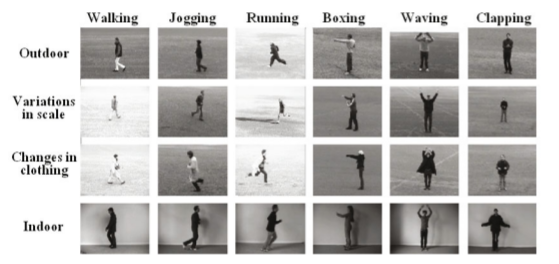
\includegraphics[width=0.85\columnwidth]{Chapters/photos/dt1.png}
\decoRule
\caption[A visualization of the KTH dataset \cite{schuldt2004recognizing}.]{A visualization of the KTH dataset \cite{schuldt2004recognizing}.}
\label{fig:datasetset1KTH}
\end{figure}\\

\section{Pre-processing of data}
For each experiment we split the data into three divisions: training split with examples used for training the classifier, validation split used to tune the parameters such as learning rate, regularization rate, optimization, etc. and test splits which contain data used for final assessment of the performance.\\

\begin{figure}[th]
\centering
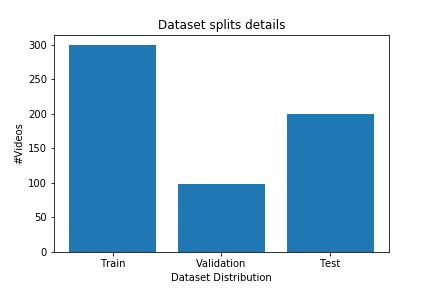
\includegraphics[width=0.83\columnwidth]{Chapters/photos/ds.png}
\decoRule
\caption[An illustration of the data splits method.]{An illustration of the data splits method.}
\label{fig:trainvalidtest}
\end{figure}\\

Technically, we create a program that take input the video directory. We then randomly dividing the whole data into 50\% for training equal to 300 videos, and 30\% for testing equal to 200 videos. Next, we take 25\% of the training data for validation. Finally, any remaining video is used for training the model. Refer to Figure ~\ref{fig:trainvalidtest} for visualization.

\subsection{Preprocessing Operation}
Video frame preprocessing is the term for operations on video frames or images at the lowest level of analysis. Generally, the aim of preprocessing operators
for HAR is to improve the image data by suppressing undesired degradations and simultaneously enhancing specific relevant features.\\

In this section, we describe and explain our robust preprocessing operators that are
important for enhancing video features and helpful in suppressing information that is not relevant in the video. This pipeline consists of 4 steps as follow.\\

\begin{figure}[ht]
\centering
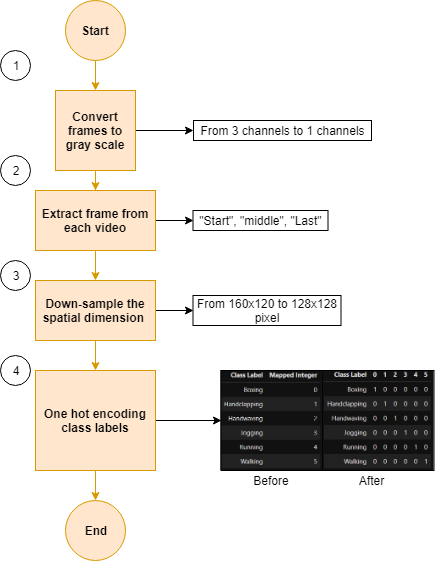
\includegraphics[width=0.5\columnwidth]{Chapters/photos/fc.png}
\decoRule
\caption[A flowchart show the steps followed to preprocess the video before feeding them to the network.]{A flowchart show the steps followed to preprocess the video before feeding them to the network.}
\label{fig:datapreprocessingpipeline}
\end{figure}\\

To simplify the computation power and complexity, we first take all frames in each video and convert them to grayscale. Although, KTH data are grayscale as described by the authors and motions in general are not defined by colors aspects, still a grayscale conversion is important to the system for final assessment and evaluation. Secondly, we program three options to extract video frames to facilitate the frame extraction, such as "start", "middle", "last". For our experiments, we know that action like "walking", "running" and "jogging" doesn't happen at the beginning of these videos which create lots of redundant and empty frames. This might affect the performance of our model. For that reason, we use the "middle" to extract the frames. We assume that each video has \textbf{M} frames in total, and the selected frames are defined by \textbf{N}. There are (\textbf{M} - \textbf{N}) frames. We would remove the first and last $\LARGE \frac{M-N}{2}$. Next, we downsample to spatial dimension from 160x120 to 128x128 pixel resolution, to ensure that all data have similar input size. Finally, we convert the input categorical labels into integers, then we apply One hot encoding on these integers labels, where the encoded labels (integers) are converted to binary variable that represent each categorical classes. Refer to Table ~\ref{tb:onehotencoding} and Table ~\ref{tb:onehotencoding2} for an illustration of One Hot Encoding and Figure ~\ref{fig:datapreprocessingpipeline} for visualization of the data pre-processing flowchart.

\begin{table}[ht]
\caption{How the class labels are mapped before one-hot encoding}
\centering
\begin{tabular}{|c|c|}
\hline
\textbf{Class Label} & \textbf{Mapped Integers} \\ \hline
Boxing               & 0                        \\ \hline
Handclapping         & 1                        \\ \hline
Handwaving           & 2                        \\ \hline
Walking              & 3                        \\ \hline
Jogging              & 4                        \\ \hline
Running              & 5                        \\ \hline
\end{tabular}

\label{tb:onehotencoding}
\end{table}
\begin{table}[ht]
\caption{How the class labels are mapped after one-hot encoding.}

\centering
\begin{tabular}{|c|c|c|c|c|c|c|}
\hline
\textbf{Class Label} & \textbf{0} & \textbf{1} & \textbf{2} & \textbf{3} & \textbf{4} & \textbf{5} \\ \hline
Boxing               & 1          & 0          & 0          & 0          & 0          & 0          \\ \hline
Handclapping         & 1          & 1          & 0          & 0          & 0          & 0          \\ \hline
Handwaving           & 2          & 0          & 1          & 0          & 0          & 0          \\ \hline
Walking              & 3          & 0          & 0          & 1          & 0          & 0          \\ \hline
Jogging              & 4          & 0          & 0          & 0          & 1          & 0          \\ \hline
Running              & 5          & 0          & 0          & 0          & 0          & 1          \\ \hline
\end{tabular}
\label{tb:onehotencoding2}
\end{table}


\section{Model Architecture 1: CNN}
In this section, we introduced our proposed CNN architecture, and we give a comprehensive explanation of our methodology. First, we briefly described the fundamental of a CNN model. Then we explain the reason behind the choice of activation function, regularization method, global average pooling (GAP) layer and its advantages toward the model parameters. Finally, we provide a visualization for the overall architecture.  

\subsection{What is a CNN model?}
CNN is a category of neural networks that recently have proven very effective in areas such as supervised classification and image recognition. CNNs have been successful in identifying the object at a microscopic scale empowering vision in medical images and nanotechnology applications. Convolutional networks were first introduced by \cite{lecun1989generalization}, as a special kind of network for processing data that has an understandable grid-like topology.\\

Convolution helps a machine learning system by leveraging three critical ideas, such as sparse interactions, equivariant representations and parameter sharing. Sparse interactions refer to sparse connectivity or sparse weights, and this is accomplished by making the kernel smaller than the inputs. For example, an input image might contain thousands of pixels, and the detection is performed on small meaningful features such as edges with kernels that occupy only tens or hundreds of pixels. This means that storing fewer parameters and operations, will both reduces the memory requirements of the model and improves its statistical efficiency. Parameter sharing refers to the usage of the same parameter for more than one function in a model. This means that the convolution operation learns a separate set of parameters for every location. This does not affect the run-time of forwarding propagation, but it does reduce the storage requirements of the model to $k$ parameters. As a result, convolution is then extremely efficient than dense matrix multiplication regarding memory requirements and statistical efficiency. Figure ~\ref{fig:la} graphically represents how parameter sharing works.
\begin{figure}[th]
\centering
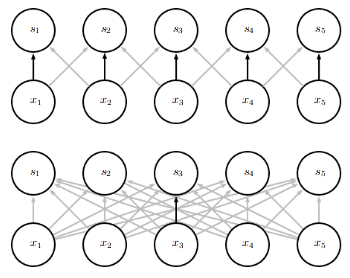
\includegraphics{Figures/ps}
\decoRule
\caption[The black arrow indicates the connections that use a particular parameter in two different model. \textit{(Top)} Black arrows indicate the usage of the centre of a three element kernel in a convolutional model. Due to parameter sharing, a single parameter is used at all input locations. \textit{(Bottom)} Black arrows indicate the usage of the central element of the weight matrix in a fully connected model. The model has no parameter sharing. As a result, the parameter is used only once \parencite{goodfellow2016deep}]{The black arrow indicates the connections that use a particular parameter in two different model. \textit{(Top)} Black arrows indicate the usage of the centre of a three element kernel in a convolutional model. Due to parameter sharing, a single parameter is used at all input locations. \textit{(Bottom)} Black arrows indicate the usage of the central element of the weight matrix in a fully connected model. The model has no parameter sharing. As a result, the parameter is used only once \parencite{goodfellow2016deep}}
\label{fig:la}
\end{figure}\\

As a result, sparse connectivity and parameter sharing can dramatically improve the efficiency of a linear function for detecting significant edges in an image. Figure ~\ref{fig:lala} shows both of these first two principles in action.\\

In convolution, the form of parameter sharing causes the layers to have a property called equivariance to translation. Generally, a function is equivariant means that if the input changes, the output changes in the same way. With images, convolution creates the 2D map of where certain features appear in the input, if the object is moved in the input, its representation will move the same amount in the output. For example, when performing image processing, it is useful to detect edges in the first layer of a convolutional layer.\\

In the image the same edges may appear more or less everywhere, for that reason, it is practical to share parameter across the entire image. However, this is not the case when processing images that are cropped to be centred on an individual face. That is because different features should be extracted at different locations. For example, the part of the network processing the top of the face needs to find eyebrows, while the part of the network processing the bottom of the face needs to look for a chin. Convolution is not equivariant to some other transformations, such as changes in the scale or rotation of an image, and other mechanisms are necessary for handling these kinds of transformations.\\

\begin{figure}[th]
\centering
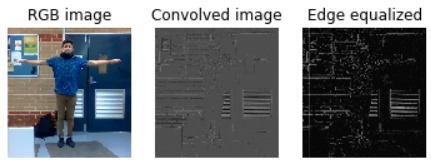
\includegraphics{Figures/edgedetection.png}
\decoRule
\caption[The image in the middle was formed by taking each pixel in the original image and subtracting the value of all vertically oriented edges in the input image. All images are 721 pixels tall. The input image is 681 pixels wide, while the output images are 680. This transformation can be described by a convolutional kernel containing two elements and requires 721*680*3=1,470,840 floating-point operations to compute using convolution. To describe the same transformation with a matrix multiplication would take 681*721*680*721, or over 240 billion entries in the matrix, making the convolution 240 billion times more efficient for representing this transformation]{The image in the middle was formed by taking each pixel in the original image and subtracting the value of all vertically oriented edges in the input image. All images are 721 pixels tall. The input image is 681 pixels wide, while the output images are 680. This transformation can be described by a convolutional kernel containing two elements and requires 721*680*3=1,470,840 floating-point operations to compute using convolution. To describe the same transformation with a matrix multiplication would take 681*721*680*721, or over 240 billion entries in the matrix, making the convolution 240 billion times more efficient for representing this transformation}
\label{fig:lala}
\end{figure}\\

A CNN model is made up of Layers. Every layer transforms an input 3D volume of activations to an output 3D volume with some differentiable function that may or may not have parameters as well as additional hyperparameters. There are distinct types of layers such as Convolutional layer, Pooling layer and a fully connected layer. Stacking these layers together will form a convolutional neural network architecture. In the following subsections, we describe each individual layers and the details for their hyperparmeters and their unique connectivities. Figure ~\ref{fig:standardCNN} presents a CNN model architecture with all its required layers and mathematical operations.
\begin{figure}[th]
\centering
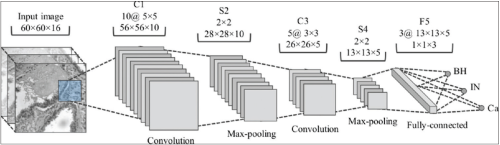
\includegraphics{Figures/cnn}
\decoRule
\caption[A visualization of a CNN architecture consisting of an input image of 60*60*16 followed by two convolutional layers and two max pooling layers and then followed by a fully connected layer \parencite{haj2017classifications}]{A visualization of a CNN architecture consisting of an input image of 60*60*16 followed by two convolutional layers and two max pooling layers and then followed by a fully connected layer \parencite{haj2017classifications}}
\label{fig:standardCNN}
\end{figure}\\

\subsection{Model Architecture}
This model is specifically designed to process RGB videos data. We choose to apply 3D CNN models inspired by popular the pretrained model AlexNet by \cite{krizhevsky2012imagenet}, due to its reputable performance on several types of data specially HAR related tasks. Since our videos are 3 dimensional, including time, we believe that 3D convolutional layers are more efficient due to their capabilities in learning spatial features.\\

Technically, our model consists of 5 convolutional groups, each of these groups has one or more convolutional layers, one max pooling layer and a LeakyReLU function, followed by a global average pooling (GAP), two fully connected layer, a dropout  layer and a  softmax layer to predict the final classification score of each class. Several decisions was made to found the best combination of layers. These decisions range from:
\begin{enumerate}
    \item Choosing the best sliding window filter for each convolutional layer and max pooling layer.
    \item Find the best combination of CNN layer that downsample the input frames to an even size before flatten these image's pixels to a 1D array.
    \item Find the best regularization method to reduce overfitting and vanishing gradient.
    \item Finding the right activation function to classify the spatial features.
    \item Finding the best optimization method that speed up the training time without affecting the model accuracy.
\end{enumerate}
The next section (sections 2.4.3-2.4.6) give a step by step explanation of these design decisions.
\begin{figure}[ht]
\centering
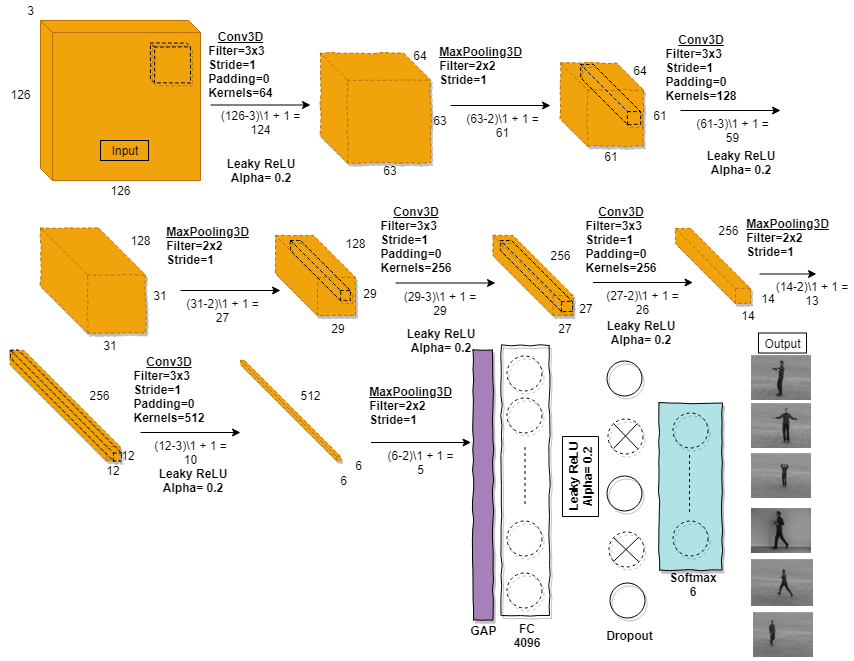
\includegraphics[width=0.85\columnwidth]{Figures/nn2.png}
\decoRule
\caption[A visualization of our proposed CNN architecture.]{A visualization of our proposed CNN architecture.}
\label{fig:la2}
\end{figure}

\subsection{Convolutional Layer}
\hspace{5mm} The convolutional layer is the core building block of a CNN model that does most of the heavy computation. In this section we will discuss the mathematical process of a convolutional layer.\\

Convolutional layer is a set of parameters consist of a set of learnable filters, where every filter is spatially along the width and the height, and also extend through the full depth of the input volume. The first filter has size of $3x3x1$ where $3$ is the pixels of the width and height of the image, and $1$ is its color channels, such as 1 grayscale and 3 for RGB. During the forward pass, we convolve each filter across the height and width of the input volume and calculate dot products between the entries of the filter and the input at any position. Since we are using 3D convolutional, a 3D activation map is produced everytime the filter slides over the input volume. The activation map give the responses of that filter at every spatial position. The network will then learn filters that activate when they spot some type of visual feature or pattern such as edge or blotch of some color on the first layer. On the other hand, each of these convolutional filters hold a stride and zero-padding. Stride is an instruction for the filter to shift at a certain unit at a time, in our case we set the stride to 1. Stride is normally set in a way so that the output volume is an integer and not a fraction. Zero-padding add zeros around the outside of the input volume so that the convolutions end up with the same number of outputs as inputs. For that reason, we set zero-padding to zero, to preserve as much as information about the original frame.\\
We calculate the size of the convolutional layer output tensor based on the this formula 

\begin{equation}
    W_{2}=\frac{W1-F+2P}{S} +1
\end{equation}

\hspace{5mm} Where \textbf{W2} is the size of the output image, \textbf{W1} is the size of the input image, \textbf{F} is the receptive field size of the Conv Layer neurons, \textbf{P} is the amount of zero padding used, and \textbf{S} is the stride.\\

\begin{figure}[ht]
\centering
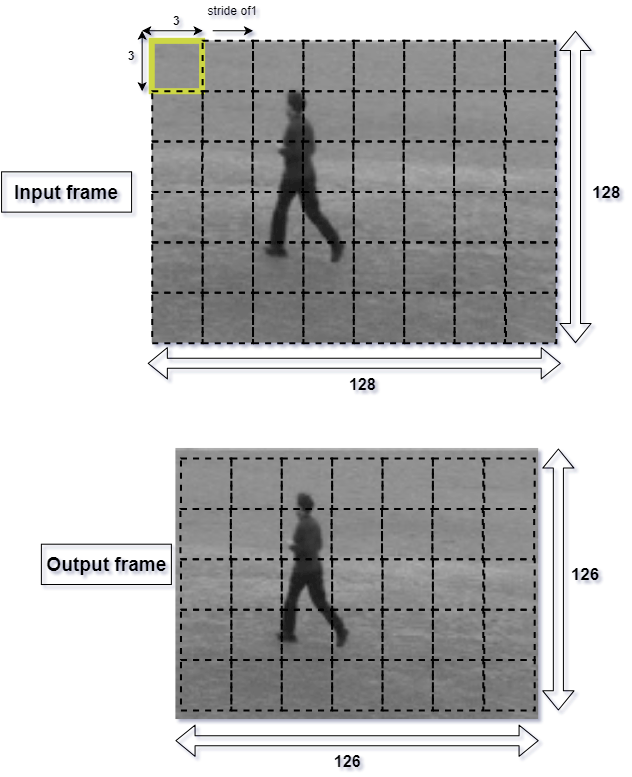
\includegraphics[width=0.8\columnwidth]{Figures/d1.png}
\decoRule
\caption[A visualization of the convolutional operation on one of the frame. The filter colored yellow has dimension of 3x3x1. We moved the convolutional 1 pixel at a time which is equal to stride of 1.]{A visualization of the convolutional operation on one of the frame. The filter colored yellow has dimension of 3x3x1. We moved the convolutional 1 pixel at a time which is equal to stride of 1. The output dimension are reduced from 128 to 126 pixels.}
\label{fig:la2la22}
\end{figure}

Having multiple filter in each convolutional layer produce a seperate 3D activation map for each filter. Stacking these activation maps along the depth dimension produce the output volume. Figure ~\ref{fig:la2la22} shows the convolutional operations in a 128x128 pixels frame.

\subsection{Max Pooling Layer}
\hspace{5mm} A pooling layer is another building block of a CNN and it is described as sample-based discretization process. This section describes the pooling operation of our convolutional network.\\

Convolutional networks may include local or global pooling layers which combine the outputs of neuron clusters at one layer into a single neuron in the next layer. It uses the maximum value from each of a cluster neuron at prior example, or it can also average this value. Its function is to progressively down-sample the spatial size of the representation to reduce the amount of parameters and computation in the network to learn and provides basic translation invariance to the internal representation.\\

Pooling operates independently in every depth slice of the input. The most common approach used in pooling is max pooling, also the one used in our CNN model. Max Pooling layer comes always after the convolutional operation by applying a max fitler to non overlapping subregions of the initial representation. It takes a filter of size 2x2 and stride of 1, and for each of the regions represented by the filter, it takes the maximum of that region and create a output matrix where each element is the max of the region in the original input. We calculate the size of the max pooling layer output tensor based on the formula below.

\begin{equation}
 W_{2}=\frac{W1-F}{S} +1
\end{equation}
This equation is obtained using the formula of the convolutional layer by making padding equal to zero. Refer for ~\ref{fig:maxpoolinglayervisualization} for maxpooling operation visualization.
\begin{figure}[ht]
\centering
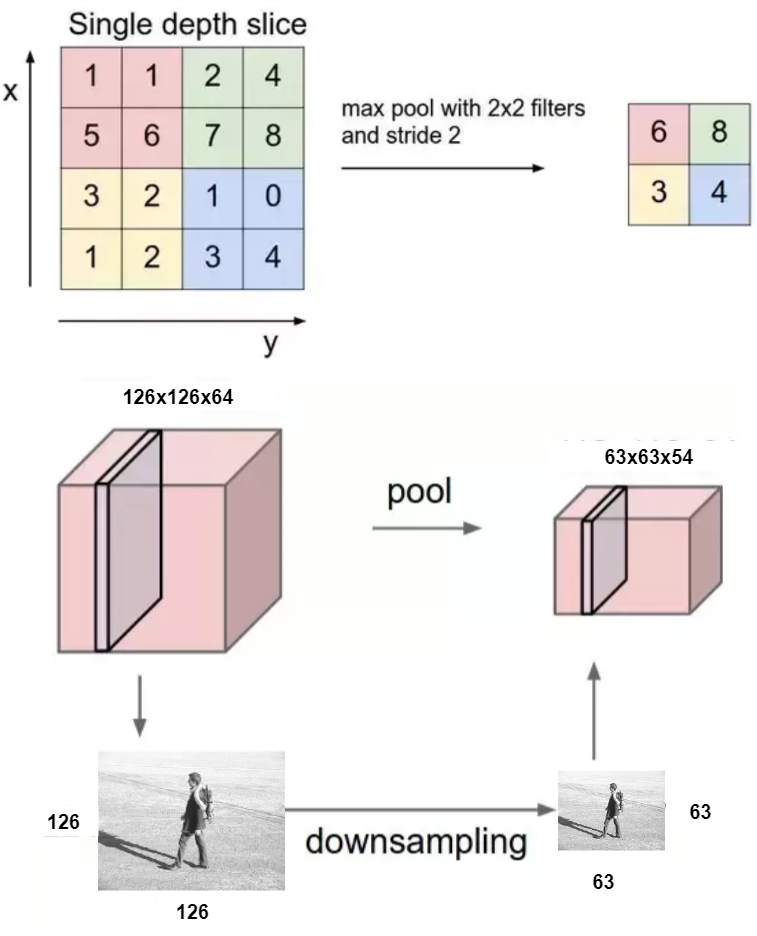
\includegraphics[width=0.6\columnwidth]{Figures/mp3.png}
\decoRule
\caption[A visualization of the max pooling operation on one of the frame. The input image has size of 126x126x64. We apply a max pooling with a filter of 2x2 with stride of 1. The output image become 63x63x64, where 64 is the kernel size.]{A visualization of the max pooling operation on one of the frame. The input image has size of 126x126x64. We apply a max pooling with a filter of 2x2 with stride of 1. The output image become 63x63x64, where 64 is the kernel size.}
\label{fig:maxpoolinglayervisualization}
\end{figure}

\subsection{Activation Function - LeakyReLU}

\begin{figure}[ht]
\centering
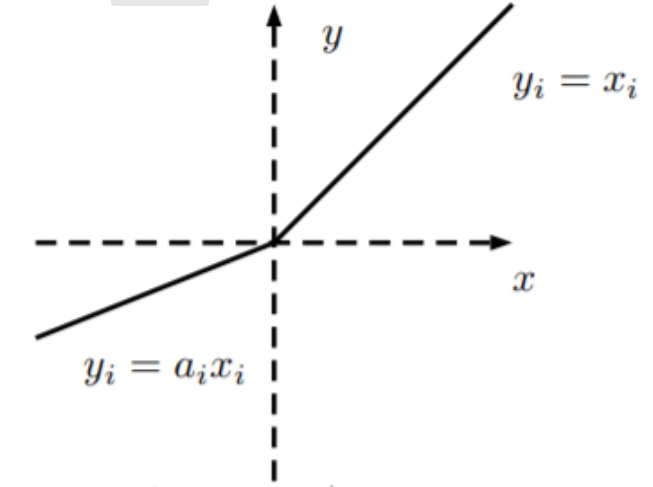
\includegraphics[width=0.6\columnwidth]{Figures/leakyrelu.PNG}
\decoRule
\caption[A visual representation of the Leaky ReLU activation function.]{A visual representation of the Leaky ReLU activation function.}
\label{fig:leakyreluactivationfunctions}
\end{figure}

Leaky ReLU was first introduced by \cite{xu2015empirical}. it is convention to apply a non linear layer or activation function immediately after every convolutional layer. The purpose of this layer is to introduce non linearity to a system that basically has just been computing linear operations during the convolutional layers. In the past, non linear functions like tanh and sigmoid were used, but researchers found out that leaky rectified linear unit (ReLU) work far better because the network is able to train a lot faster without making a significant difference to the accuracy. It also help to alleviate the vanishing gradient problem, which is the issue where the lower layers of the network train very slowly because the gradient decreases exponentially through the layers.\\

The reason behind choosing  this type of activation function is avoiding vanishing gradient and overfitting. Instead of the function being zero when x$\leq$ 0, a leaky ReLU will instead have a small negative slope (approximetly of 0.01 or more), as shown in Equation ~\ref{eq:la} and ~\ref{eq:la3} below.
\begin{equation}
\label{eq:la}
   \large  y_{i} = x_{i}, & x\geq 0
\end{equation}

\begin{equation}
\label{eq:la3}
   \frac{x_{i}}{a_{i}}, & x< 0
\end{equation}
\hspace{5mm} Here $y_{i}$, is the input of the non linear activation function of the \textit{i}th channels, and $a_{i}$ is a coefficient  controlling the slope of the negative part. The subscript \textit{i} in $a_{i}$ indicates that we allow the non linearity function to vary on different channels. Refer to Figure ~\ref{fig:leakyreluactivationfunctions} for Leaky ReLU activation function visualizayion.

\subsection{Regularization - Dropout}
Dropout is a stochastic regularization technique was first studied by \cite{srivastava2014dropout}. The term "dropout" refers to removing out units in the hidden layer of a network, with all its incoming and outgoing connections as shown in Figure ~\ref{fig:r}. In practice, the choice of dropping unit is random with a fixed probability $\large \rho$ independent of the other unit, where $\large \rho$ can be chosen using a validation set or can simply be set at 0.5. This makes their contribution to the activation temporally removed on the forward pass and any weight updates are not applied on the backward pass. These neurons become less sensitive to the weight update of the model. One of the advantages of using Dropout is generating better generalization and reduce over-fitting the training data.\\

In our experiment, we dropped approximately 20\% of
the hidden layers to make other neurons step in and handle the representation required to make predictions for the
missing neurons. This result in multiple independent internal representations being learned by the network after each
iteration.

\begin{figure}[ht]
\centering
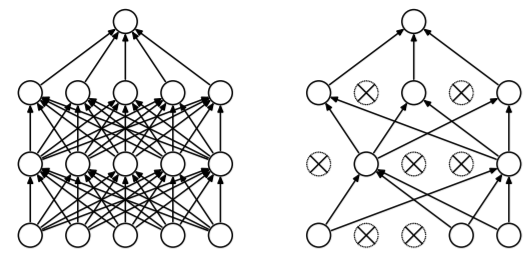
\includegraphics[width=0.6\columnwidth]{Figures/do}
\decoRule
\caption[\textbf{Left:} shows a standard neural network with 2 hidden layer. \textbf{Right:} shows the same network but with dropout applied to its hidden layers.]{\textbf{Left:} shows a standard neural network with 2 hidden layer. \textbf{Right:} shows the same network but with dropout applied to its hidden layers.}
\label{fig:r}
\end{figure}

\subsection{Model Parameters}
Generally, each layer has two kinds of parameters such as weights and biases. Hence, the sum of these two represents the model parameters. In practice, the number of parameters is proportional to the model complexity and model performance. On the other hand, having more parameters makes the model flexible and behave better with regularization and fine tuning.\\

In our architecture Figure ~\ref{fig:la2}, the input is an image of size 128*128*3. After Conv3D-1, the size of changes to 126x126x96 which is transformed to 63x63x96 after MaxPool3D-1. After Conv3D-2, the size changes to 61x61x128 and following MaxPool3D-2 it changes to 31x31x128. Conv3D-3 transforms it to a size of 29x29x256, then Conv3D-4 downsample this image to 27x27x256 and MaxPool3D-3 changes the size to 14x14x256, then Conv3D-5 reduce it to 12x12x512. Finally, GAP reduces the size to 6x6x512. This image feeds into FC-1 which transforms it into a vector of size 4096×1. The size remains unchanged through Dropout, and finally, we get the output of size 6×1 after Softmax layer. We calculate these two parameters according to following formulas.\\
\begin{itemize}
    \item \textbf{Number of Parameters of a Convolutional Layer}
    \begin{equation}
         W_{c} = O^{2} \ast N \ast F
    \end{equation}
\begin{equation}
     B_{c} = F
\end{equation}
\begin{equation}
     P_{c} = W_{c} + B_{c}
\end{equation}
Where:\\
\begin{itemize}
    \item \textbf{$W_{cf}$}: Number of weights of a fully connected Layer which is connected to a Convolutional Layer.
    \item \textbf{$B_{cf}$}: Number of biases of a fully connected Layer which is connected to a Convolutional Layer.
    \item \textbf{O}: Size (width) of the output image of the previous Convolutional Layer.
    \item \textbf{N}: Number of kernels in the previous Convolutional Layer.
    \item \textbf{F}: Number of neurons in the fully connected Layer.
    
\end{itemize}
    \item \textbf{Number of Parameters of a Max Pooling Layer}: There are no parameters associated with a Max Pooling layer. The pool size, stride, and padding are hyper-parameters.
    
    \item \textbf{Number of Parameters of a Fully Connected Layer}: There are two kinds of fully connected layers in a CNN. The first FC layer is connected to the last Conv Layer, while later FC layers are connected to other FC layers.
    \begin{equation}
 W_{cf} = O^{2} \ast N \ast F
\end{equation}
\begin{equation}
 B_{cf} = F
\end{equation}
\begin{equation}
 P_{cf} = W_{cf} + B_{cf}
\end{equation}

Where:\\
\begin{itemize}
    \item \textbf{$W_{cf}$}: Number of weights of a fully connected Layer.
    \item \textbf{$B_{cf}$}: Number of biases of a fully connected Layer.
    \item \textbf{O}: Size (width) of the output image.
    \item \textbf{N}: Number of kernels in the previous Convolutional Layer.
    \item \textbf{F}: Number of neurons in the fully connected Layer.
\end{itemize}
\end{itemize}
The total number of parameters in our model is the sum of all parameters in the 5 Conv Layers + 1 FC Layers + Dropout Layer. It 8,543,110 in total. Table ~\ref{tab:CNNmodelarchi} provides a summary of our CNN model parameters.


\begin{table}[ht]
\caption{Total number of parameters in our proposed neural network architecture.}
\centering
\begin{tabular}{|c|c|c|c|c|}
\hline
\textbf{Layer  name} & \textbf{Image} & \textbf{Weight} & \textbf{Biases} & \textbf{Params} \\ \hline
Input image & 128x128x1 & 0 & 0 & 0 \\ \hline
Conv3D & 126x126x64 & 576 & 64 & 1792 \\ \hline
MaxPool3D & 63x63x64 & 0 & 0 & 0 \\ \hline
Conv3D & 61x61x128 & 1152 & 128 & 221312 \\ \hline
MaxPool3D & 31x31x128 & 0 & 0 & 0 \\ \hline
Conv3D & 29x29x256 & 2304 & 256 & 884,992 \\ \hline
Conv3D & 27x27x256 & 2304 & 256 & 1,769,728 \\ \hline
MaxPool3D & 14x14x256 & 0 & 0 & 0 \\ \hline
Conv3D & 12x12x512 & 0 & 0 & 0 \\ \hline
MaxPooling3D & 6x6x512 & 0 & 0 & 0 \\ \hline
GAP & 512x1 & 0 & 512 & 0 \\ \hline
Dense & 4,096x1 & 4,096,000 & 4,096 & 2,101,248 \\ \hline
Dropout & 4,096x1 & 0 & 4,096 & 0 \\ \hline
Output & 6 & 0 & 0 & 24582 \\ \hline
Total Params & \multicolumn{4}{c|}{8,543,110} \\ \hline
\end{tabular}
\label{tab:CNNmodelarchi}
\end{table}\hfill


\subsection{Global Average Pooling}
\hspace{5mm} Conventional CNN perform convolutional in the lower layers of the network. As a results, \cite{lin2013network} proposed a new strategy called global average pooling, as a replacement to the traditional fully connected layer. GAP layer generate one feature map for each corresponding category of the classification. That's said, instead of adding fully connected layers on top of the feature maps, we take the average of each feature map, and the resulting vector is fed directly into the softmax layer for final prediction. One advantage of GAP layers is that it is more native to the convolution structure by enforcing correspondences between
feature maps and categories. Thus the feature maps can be easily interpreted as categories confidence
maps. Another advantage is that there is no parameter to optimize in the global average pooling
thus over-fitting is avoided at this layer. Furthermore, global average pooling sums out the spatial
information, thus it is more robust to spatial translations of the input.\\

In our experiment, the number of parameters increases in each layer. An architecture like this is more likely to over-fit during training. For that reason, we used GAP layer to reduce our model parameters before it reaches fully connected layers. As an example, the number of parameters in our model are reduced from 3,539,456 to 2,101,248 after GAP is applied Table ~\ref{tab:CNNmodelarchi}. Figure ~\ref{fig:gap} shows tensor with dimensions h*w*d is reduced in size to have dimensions 1*1*d. GAP layers reduce each h×w feature map to a single number by simply taking the average of all h*w values.

\begin{figure}[ht]
\centering
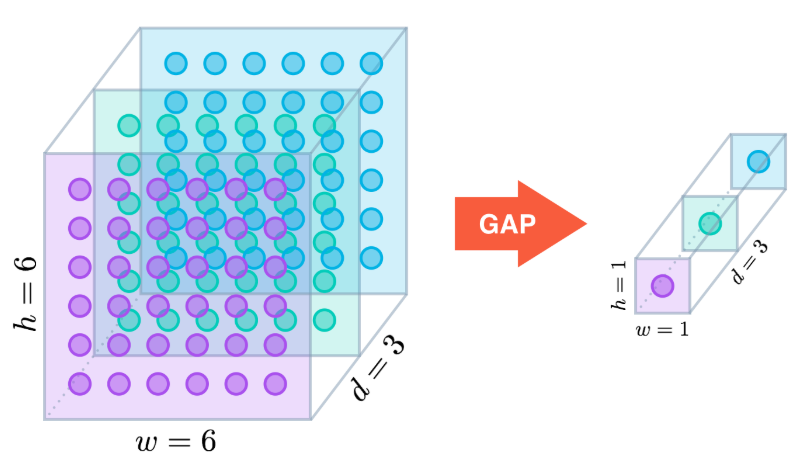
\includegraphics[width=0.6\columnwidth]{Figures/gap}
\decoRule
\caption[An example of a GAP applied on a 3D image \cite{lin2013network}.]{An example of a GAP applied on a 3D image \cite{lin2013network}.}
\label{fig:gap}
\end{figure}

%----------------------------------------------------------------------------------------


\section{Model Architecture 2: CNN-LSTM}
In this section, we introduce Recurrent neural network (RNN) architecture, and we give a comprehensive explanation of our methodology using CNN and RNN in one model. We first, describe briefly the fundamental of a RNN model, then we explain the reason behind the choice of our activation function, memory layer, wrapping the entire architecture with Time Distributed layer and the advantage of using batch normalization to speed up the training. Finally, we provide a visualization for the overall architecture.

\subsection{What is a RNN model?}

RNN are a family of neural network designed to recognize patterns in sequences of data, such as text, genomes and handwriting etc. These algorithms take time and sequence into account, they have a temporal dimension.
RNN was first introduced by \cite{rumelhart1986learning}, to be one of the most powerful and useful type of neural network, alongside the attention mechanism and memory networks. RNNs are applicable even to images, which can be decomposed into a series of patches and treated as a sequence.
Since recurrent networks possess a certain type of memory, and memory is also part of the human condition, we’ll make repeated analogies to memory in the brain.\\

RNN helps a machine learning system by leveraging one of the early ideas found in statistical model of the 1980s such as sharing parameters across different parts of a model. Parameter sharing makes it possible to extend and apply the model to examples of different forms and lengths and generalize across them. Such sharing is particularly important when a specific piece of information can occur at multiple positions within the sequence. Recurrent networks share parameters in a different way. Each member of the output is a function of the previous members of the output. Each member of the output is produced using the same update rule applied to the previous outputs.This recurrent formulation results in the sharing of parameters through a very deep computational graph.\\

While CNNs are effective at learning spatial features in single independent frames, a recurrent layer excels at integrating temporal context. \cite{tripathi2016context} defined a neural network architecture where the frame-by-frame object predictions of a pre-trained convolutional neural network where used as inputs to a recurrent layer. A similar approach is taken in these experiments, with the exception that the convolutional network is fine-tuned jointly with the training of the recurrent layer. The communication between the CNN and the RNN is learned concurrently with the optimization and is not limited to passing actual object class predictions. The RNN outputs the final predictions for each frame while taking previous frames into account using memory layer. Another example of CNN-RNN model, is the capability of predicting objects’ velocity vectors in the image plane. By allowing detections from previous frames to flow to the current frame via recurrent connections in the RNN layers, the network can keep track of moving objects across time and give estimates for the velocity.\\

The recurrent neural network is represented as shown in Figure ~\ref{fig:gap1}, and also shows the different types of RNN architecture in Figure ~\ref{fig:RNNmanytoonoetypes}. Each node at a time step takes an input from the previous node and this can be represented using a feedback loop. We can unfurl this feedback loop and represent it as shown in the figure below. At each time step, we take an input $x_{i}$ and $a_{i-1}$ (output of the previous node) and perform computation on it and produce an output $h_{i}$. This output is taken and given to the next node. This process continues until all the time steps are evaluated. In the following subsections, we describe each important layer that make our network unique and different from the previous architecture and the details for their hyper-parmeters and their unique connectivities.

\begin{figure}[ht]
\centering
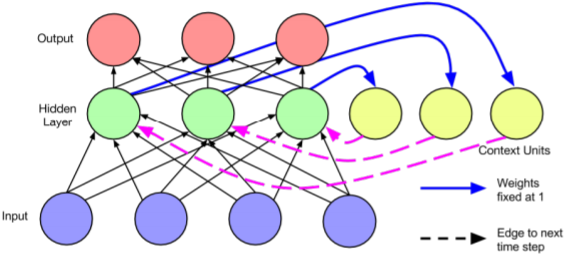
\includegraphics[width=0.60\columnwidth]{Figures/rnn}
\decoRule
\caption[An example of a recurrent neural network as described by \cite{elman1990finding}. Hidden
units are connected to context units, which feed back into the hidden units at
the next time step \citep{lipton2015critical}.]{An example of a recurrent neural network as described by \cite{elman1990finding}. Hidden
units are connected to context units, which feed back into the hidden units at
the next time step \citep{lipton2015critical}.}
\label{fig:gap1}
\end{figure}


\begin{figure}[ht]
\centering
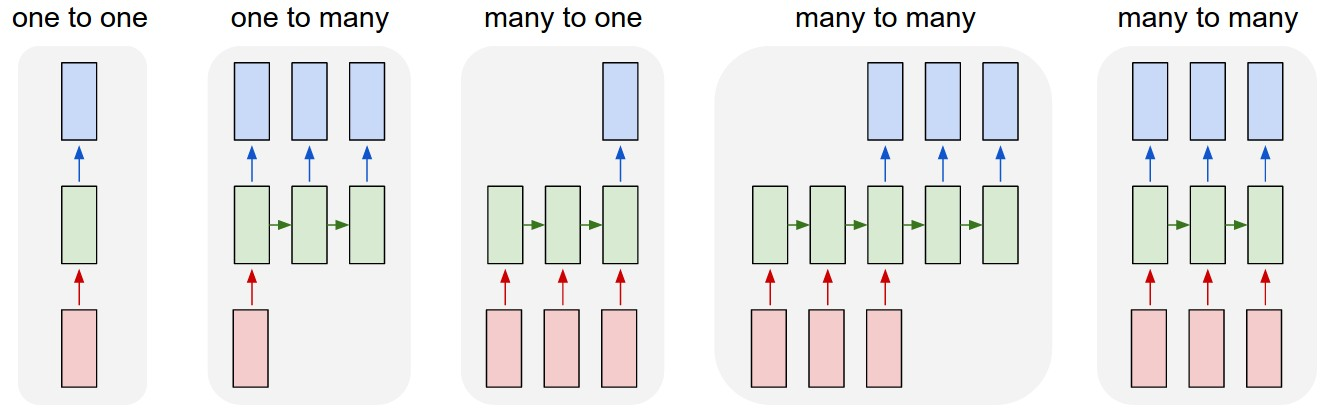
\includegraphics[width=0.8\columnwidth]{Figures/rn1}
\decoRule
\caption[A visualization of the most used RNN architectures. Red rectangles
correspond to inputs, Blue rectangles to outputs and green rectangles to the entire hidden state of the neural network. \textbf{One to one} Represents a conventional  feedforward networks. \textbf{One to many} Text and video classification are tasks in which a sequence is mapped to one fixed length vector. \textbf{Many to one}
Image captioning presents the converse case, where the input image is a single
non-sequential data point. \textbf{Many to many} This architecture has been used for natural language translation, a sequence-to-sequence task in which the two sequences may
have varying and different lengths. \textbf{Many to many} This architecture has been used to learn
a generative model for text, predicting at each step the following character \citep{lipton2015critical}.]{A visualization of the most used RNN architectures. Red rectangles
correspond to inputs, Blue rectangles to outputs and green rectangles to the entire hidden state of the neural network. \textbf{One to one} Represents a conventional  feedforward networks. \textbf{One to many} Text and video classification are tasks in which a sequence is mapped to one fixed length vector. \textbf{Many to one}
Image captioning presents the converse case, where the input image is a single
non-sequential data point. \textbf{Many to many} This architecture has been used for natural language translation, a sequence-to-sequence task in which the two sequences may
have varying and different lengths. \textbf{Many to many} This architecture has been used to learn
a generative model for text, predicting at each step the following character \citep{lipton2015critical}.}
\label{fig:RNNmanytoonoetypes}
\end{figure}

\subsection{Model Architecture}
This model architecture in Figure ~\ref{fig:lstmcnn} is an improvement of the previous model Figure ~\ref{fig:la2}. It consists of two phases: CNN and RNN-LSTM. Because our dataset consists of sequence of videos, a CNN with memory layers are used to process these sequences and learn spatial and temporal features from the videos.\\

The CNN model consists of one convolutional layers with 3x3 filter and a stride of 1, followed by a batch normalizationl layer for regularization, then using a ReLU as activation function, and max pooling layer with 2x2 filer and stride of 1, and adding Dropout as a second regularize with 0.25 dropping rate. These 4 layers are being repeated 3 times to downsample the image. After that, we add two fully dense (fully connected) layer each with 256 and 128 neurons respectively. For the second phase of this network, we build two networks of LSTM layers that take the CNN vector as input. This LSTM layers consists of a forget layer that remember the sequence of each frame and apply a tanh as activation function. Next, we know that the first layer is forward sequence while the second layer is a backward sequence. As a results, we concatenare these two layers, and apply a softmax layer that hold the action classes of the dataset. 
\begin{figure}[ht]
\centering
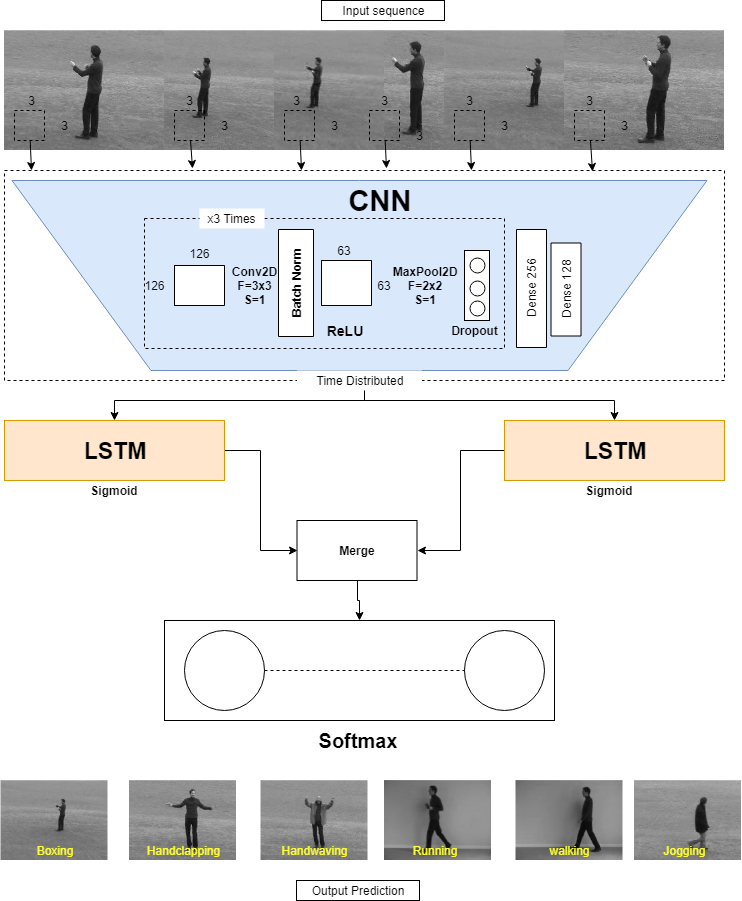
\includegraphics[width=0.75\columnwidth]{Figures/cnnlstm.png}
\decoRule
\caption[A visualization of our proposed CNN-LSTM model.]{A visualization of our proposed CNN-LSTM model.}
\label{fig:lstmcnn}
\end{figure}


\subsection{Long Short Term Memory}
\cite{hochreiter1997long} introduced the LSTM model, an extension of RNN, which stands for Long short term memory, primarily in order to overcome the problem of vanishing gradients and long-term dependency problem by explicitly learning when to modify the hidden state via gates.\\

Simple recurrent neural networks have long-term memory in the form of weights.
The weights change slowly during training, encoding general knowledge about
the data. They also have short-term memory in the form of ephemeral activation's, which pass from each node to successive nodes. The LSTM model
introduces an intermediate type of storage via the memory cell. A memory cell
is a composite unit, built from simpler nodes in a specific connectivity pattern,
with the novel inclusion of multiplicative nodes, represented by the
letter $\prod$ like in Figure ~\ref{fig:lstm}.\\

There are one input node, internal state and three gates: forget gate, input gate and output gate, each of which acts as a one layer neural network on its own.
\begin{itemize}
    \item \textbf{Input node}\\
    Takes activations in the standard way from the input layer at the current time step and along recurrent edges from the hidden layer at the previous time step. The output of each gate is limited to [0, 1] via a sigmoid activation and all gates observe both the previous hidden state and the current LSTM layer input.
    
\item \textbf{Input gate}\\
Controls when to use information present in the input. Its value is used to multiply the value of another node. It is a gate in the sense that if its value is zero, then flow from the other node is cut off. If the value of the gate is one, all
flow is passed through. The value of the input gate $i_{i}$ multiplies the value
of the input node

\item \textbf{Internal state}\\
The internal state $s_{c}$ has a self-connected recurrent edge
with fixed unit weight. Because this edge spans adjacent time steps with
constant weight, error can flow across time steps without vanishing or exploding. This edge is often called the constant error. In vector
notation, the update for the internal state is presented in Equation \ref{equation2.11}:
\begin{equation}\label{equation2.11}
     s^{(t)}=g^{(t)}\odot i^{(t)}+ s^{(t-1)}
\end{equation}

\item \textbf{Forget gate}\\
Outputs a multiplier vector for the hidden state, where zero output causes the hidden state to be discarded and one to be kept. With forget gates and according to \cite{gers1999learning}, the equation to calculate the internal state
on the forward pass is 
\begin{equation}
     s^{(t)}=g^{(t)}\odot i^{(t)}+f^{(t)}\odot s^{(t-1)}
\end{equation}
Where $s^{(t)}$ denotes internal state, $\odot$ denotes element-wise multiplication, \textbf{t} denotes the time state, \textbf{g} denotes current input for the sigmoid function, \textbf{i} and \textbf{f} denote the input gate.
\item \textbf{Output gate}
Controls how the hidden state influences the network output.
\end{itemize}

\begin{figure}[ht]
\centering
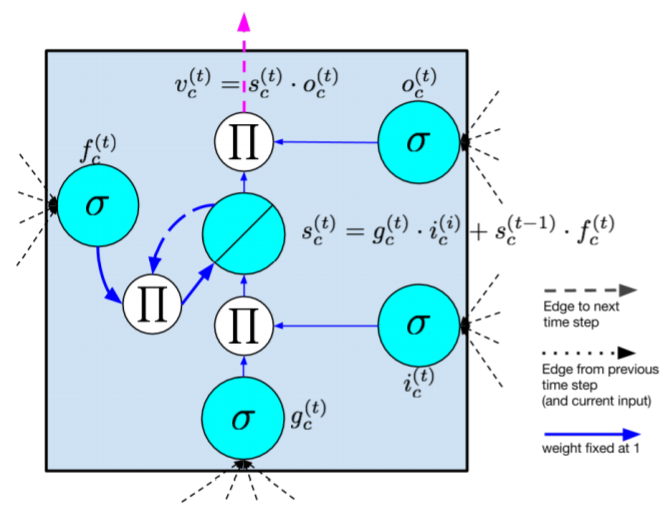
\includegraphics[width=0.80\columnwidth]{Figures/lstm}
\decoRule
\caption[An example of LSTM model as suggested by \cite{gers1999learning}.]{An example of LSTM model as suggested by \cite{gers1999learning}.}
\label{fig:lstm}
\end{figure}

All gates are learned simultaneously with the neural network, as all the
internal operations of the layer are differentiable and their effect to the final
loss function can be inferred. It can be said that during optimization the
LSTM learns which features of the input are worth keeping in the hidden
state and which features of the hidden state are not useful for prediction and
can be discarded.
By explicitly modifying the hidden state via learnable gates, the LSTM
sidesteps the vanishing gradients problem in simpler RNNs where long term
dependencies are easily lost after repeated transformations through a hidden
layer. In LSTM, the hidden state is modified only via the gates and it is very
easy for the state to flow through multiple time steps unchanged.\\

In our architecture and as shown in ~\ref{fig:lstmcnn}, there are two layers of LSTM. Both LSTMs layers are connected in parallel and take the CNN model as input and they are being concatenated afterwards. They are differentiated in that the left LSTM takes a 1x128 input dimension and output this dimension to 1x256. It has one forget bias unit, that return a sequence with a Tanh activation function and an inner Sigmoid activation function. While right LSTM layer preserves the same specification, but it reverses the given sequence. 

\subsection{Activation Function - ReLU}

\begin{figure}[ht]
\centering
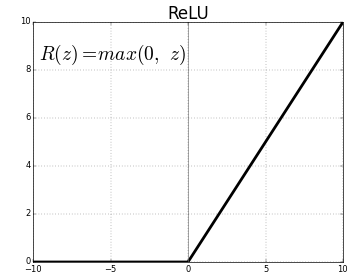
\includegraphics[width=0.80\columnwidth]{Figures/relu.png}
\decoRule
\caption[A visual representation of the ReLU activation function \cite{nair2010rectified}.]{A visual representation of the ReLU activation function \cite{nair2010rectified}.}
\label{fig:relu1}
\end{figure}
Rectified linear unit was first introduced by \cite{nair2010rectified}, as a function that have a non linear property without affecting the receptive field on the network. It's advantage consists in speeding up training and avoiding vanishing gradient, its equation can be written as below.\\

\begin{equation}\label{eq:1}
    \ y_{i} =x_{i}, & x\geq 0
\end{equation}

\begin{equation}\label{eq:2}
    0, & x \leq 0
\end{equation}

In practice, ReLU returns 0 Equation ~\ref{eq:2} if it receives any negative input, but for any positive value x it returns that value back Equation ~\ref{eq:1}. It can be written as $\large R_{(z)}=max(0,z)$, as shown in Figure ~\ref{fig:relu1} above.\\

ReLU serve two primary purposes in our model:
\begin{itemize}
    \item Help the model account for interaction effects.
    \item Help the model account for non-linear effects.
\end{itemize}
\textbf{Interactions:} The weight from the model creates interactions during training, and adding more layers and more nodes, the potential complexity of interactions only increases, in this case ReLU captures this interaction and helps in taking only positive value to help the classification model produce high accuracy for each action labels.
\textbf{Non-linearity:} In our model, we include bias for each node, which is a constant number that is determined during model training. This bias term allow us to move where the slope changes. As a result, each node change slope at different values for our output.\\

Overall, this activation have more flexibility to produce non-linearity functions and account for interactions to give better predictions, and the performance increase as the model complexity increase.

\subsection{Time Distributed Layer}
We using a CNN-RNN, that's mean, we are dealing with a sequence classification problem. It is essential to make the dense nodes of the layer identical and share the same weights and biases, using a time distributed layer applied fully connected dense on each time step and get output separately by time steps.\\

Technically, Time distributed layer applies same as a dense layer or a fully connected layer to every time step of a 3D tensor. This wrapper applies a layer to every temporal slice of an input. In our case the input, is a 3D tensor, and the dimension of index one is considered to be the temporal dimension. We used time distributed layer to all our Con3D and Max Pooling3D layers, to add an additional temporal layer. This creates a spatial vector from each frame, and associate them with an additional temporal vector for every sequence. The network then remembers each frames according to its spatial feature and appearance.

\subsection{Batch Normalization}
The distribution of each layer's inputs change during training, as the parameters of the previous layers change. This slows down the training by requiring lower learning rates and careful parameter initialization, and makes it notoriously hard to train models with saturating non-linearities. We refer to this phenomenon as internal covariate shift as suggested by \cite{ioffe2015batch}. Making normalization a part of the model architecture and performing the normalization for each training mini-batch. Batch Normalization allows us to use much higher learning rates and be less careful about initialization. It also acts as a regularizer, in some cases eliminating the need for Dropout, however, we still used dropout, as a second regularization layer. Using batch normalization, allow us to beats the original model by a significant margin.\\

We seek to reduce the internal covariate shift. By fixing the distribution of the layer inputs x as the training progresses, we expect to improve the training speed. \cite{lecun2012efficient} said that the network training converges faster if its inputs are whitened, for example, linearly transformed to have zero means and unit variances, and de-correlated. By whitening the inputs to each layer, we would take a step towards achieving the fixed distributions of inputs that would remove the ill effects of the
internal covariate shift.\\

The normalization can then be written as a transformation like in Equation \ref{normalizationfortranf} below:
\begin{equation}\label{normalizationfortranf}
     \widehat{x}=Norm(x,X)
\end{equation}
where \textbf{x} is the input layer, treated as a vector, and \textbf{X} is the set of these inputs over the training data. It depends not only on the given training example x but on all examples X, each of which depends on $\Theta$ if
x is generated by another layer. On the other hand, for back-propagation, we compute the Jacobians.

\begin{equation}\label{derivative1}
     \frac{\delta Norm(x,X)}{\delta x}
\end{equation}

\begin{equation}\label{derivative2}
    \frac{\delta Norm(x,X)}{\delta X}
\end{equation}
Where $\delta$ is derivation symbol for both Equation \ref{derivative1} and Equation \ref{derivative2}. 
The  aim is to preserve the information in the network, by
normalizing the activations in a training example relative
to the statistics of the entire training data.\\

In our experiment, batch normalization, is a part of our neural network structure, approximates this process by standardizing the activations using a statistical estimate of the mean $\widehat{E}(x)$, and standard deviation $\widehat{Var}(x)$  for each mini batch training. The below formula represents the batch normalization.
\begin{equation}
        BN\left ( x;\gamma ,\beta \right )=\gamma \frac{x-\widehat{E}(x)}{\sqrt{\widehat{Var}(x)+\epsilon }} +\beta
\end{equation}
Where $\gamma$ and $\beta$ are scale and shift parameters for the activation $x$. An identity transformation is then presented for each activation. The $\epsilon$ is a constant added as a regularization parameter for numerical stability. The division is performed element wise. $\gamma$ and $\beta$ are learned during training and fixed during inference.\\

To take full advantage of batch normalization technique, we change the network and its training parameters, such as, increasing learning rate, removing dropout, accelerate the learning rate decay, remove local response normalization, and shuffle the training example more thoroughly.

\section{Training and Testing}
Neural networks are very complex models and obtaining good results can be
difficult. This chapter describes many practical methods used to train and test our proposed neural network architecture described in Figure ~\ref{fig:la2} and Figure ~\ref{fig:lstmcnn}.

\subsection{Initialization}

Proper initialization can have a
great impact on both the speed of the training and the evaluation accuracy
of the model. Poorly initialized models can even fail to converge. Before training can begin, the initial values for the parameters of the network,
the weights and biases are selected. 
Initializing all network parameters to zero, each neuron would
receive the same learning signal from the optimizer that is minimizing the
loss, thus making all but one of them completely redundant. As such, one
goal of neural network initialization is to break symmetry between neurons. The values of W and b should be chosen so that the activations neither
vanish (approach zero) or explode (approach infinity) as they pass through
all layers in the network. We initialize the
neuron biases to zero and sample initial weights from a random distribution
such as the uniform distribution with variance by \cite{glorot2010understanding}.
\begin{equation}
    Var[W_{i}]=\frac{2}{n_{i}+n_{i-1}}
\end{equation}
In this equation $W_{i}$ is the weight, $n_{i}$ is the number of neurons on the layer $j$. The justification for this initialization is that it approximately preserves the norms of the activation vector and the error gradient. On the other hand, we initialize the weight. Refer to Equation \ref{equationbelow} below.

\begin{equation}\label{equationbelow}
     Var[W_{i}]=\frac{2}{n_{i}}
\end{equation}
The purpose is initializing the neurons biases to zero, because the ReLU halves the variance of the data, to compensate the weight.

\subsection{Optimization}
For optimization, we considered an optimization technique that minimize an objective function with respect to the network parameters. We use Stochastic gradient descent (SGD). With SGD, the gradient vectors become stochastic and fluctuate around
the real gradient. The variance of the gradients can be decreased by increasing the number of samples in the mini-batch.\\

In our experiment, SGD updates model parameters $\theta$ in the negative direction of the gradient $g$ by taking a subset or a mini-batch of data of size m

\begin{equation}\label{eq:lr}
     g=\frac{1}{m}\Delta _{\Theta }\sum _{i}L(f(x^{(i);\Theta }), y^{(i)})
\end{equation}

\begin{equation}\label{eq:the}
    \Theta =\Theta -\epsilon _{k}*g
\end{equation}
In equation ~\ref{eq:lr}, the neural network model is represented by $\large f(x^{(i)};\Theta )$. $\large x^{(i)}$ are the training data and $\large y^{(i)}$  are the training labels, the gradient of the loss L is computed with respect to model parameters $\theta$. The learning rate $\epsilon$ from equation ~\ref{eq:the} determines the size of the step that the algorithm takes along the gradient, and it also controls the size of the optimization step. If the step size is too large the optimization overshoots and can end up oscillating around a local minimum in the optimization space. If it is too small the method will take long to converge to optimal parameters. For our proposed model, we want the learning rate $\epsilon$ to satisfy the robbins-monroe conditions by \cite{lecun2015deep}.
\begin{equation}\label{eq:epr}
     \sum _{k}\epsilon _{k}=\infty
\end{equation}

\begin{equation}
    \sum _{k}\epsilon _{k}^{2}< \infty
\end{equation}
where $i$ is a scalar that grows linearly during the learning process, such as
the number of gradient updates applied thus far. The first equation ~\ref{eq:epr} dictates that the optimizer is able to travel arbitrarily long paths in the optimization
space while the second guarantees that the learning rate is decreasing at a
sufficient rate.\\

This learning rate value is set to 10e-3 with 128 mini-batches for the first CNN model, and 10e-2 with 32 mini-batches for the second CNN-LSTM model.

\subsection{Momentum}

The momentum is an exponentially decaying vector where gradients from
previous steps are accumulated. If the gradient of the objective function is
close to zero or noisy, the momentum term will help the optimizer continue in
the same direction. For example, SGD has trouble navigating ravines, which are common around local optima. In these scenarios, SGD oscillates across the slopes of the ravine while only making hesitant progress along the bottom towards the local optimum as shown in Figure ~\ref{fig:momentum} below.  It is an additional
hyperparameter to tune. The equations of gradient descent are revised as follows.
\begin{figure}[ht]
\centering
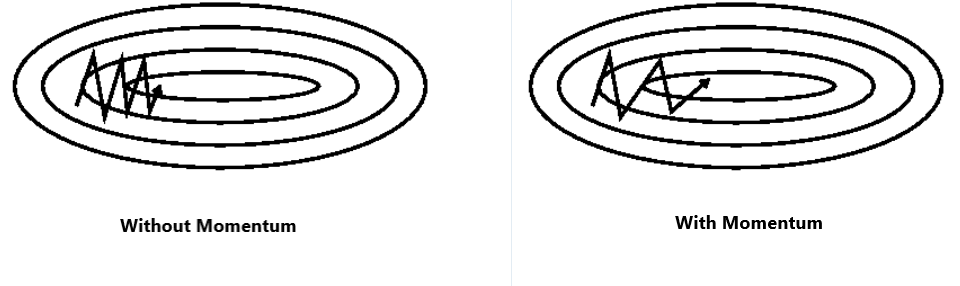
\includegraphics[width=0.80\columnwidth]{Figures/mm.png}
\decoRule
\caption[\textbf{Right:} An optimized gradient descent with momentum. \textbf{Left:} The same gradient descent but without using momentum.]{\textbf{Right:} An optimized gradient descent with momentum. \textbf{Left:} The same gradient descent but without using momentum.}
\label{fig:momentum}
\end{figure}
\begin{equation}\label{eq:eps}
     v=\alpha v-\epsilon \Delta _{\Theta }(\frac{1}{m}\sum _{i}L(f(x^{(i)};\Theta ),y^{(i)}))
\end{equation}

\begin{equation}
    \Theta =\Theta +v
\end{equation}
where $\epsilon$ $\geq$ 0 is the learning rate. Thus step size depends on how large and how aligned the sequence of gradients are.
Equation ~\ref{eq:eps} has two parts. The first term is the gradient that is retained from previous iterations. This retained gradient is multiplied by Coefficient of Momentum $\alpha$ which is the percentage of the gradient retained every iteration.\\

In our experiment, we set the momentum to 0.9 for both of our model. As a result, we gain faster convergence and reduced oscillation.


\section{Summary}
In this chapter, a step by step explanation of our proposed models was given. First, we introduced the popular KTH dataset used for this thesis. Then, we explained our data splits method used to divide the dataset into three main directories. Next, we introduced and explained our first proposed CNN model. In this method, spatial features were extracted where the action of interest is more significant. Then, we introduced and explained our second proposed model CNN-LSTM, which consist of a CNN network combined with a LSTM layer that act as memory layer. At the end, we explained our initialization and optimization method used to make both of these models converge in the global maximum at the end of the training.
%----------------------------------------------------------------------------------------

\chapter{Results and Discussions}

This chapter presents final results of our neural network frameworks. We present graphs, confusion matrices and accuracy \& loss to evaluate our model. We compared the results between these two models. We concluded this chapter with a discussion about the future direction based on the model with highest accuracy and less complexity and computation power.

\section{Results}
In this section we will report the performance of the proposed CNN and CNN-LSTM models on KTH dataset. The performance are compared between both of these models according to their accuracy, loss and confusion matrix.\\

To understand the performance and accuracy of the model, the performance are evaluated using the trained data and perform an evaluation on the test data. Since KTH dataset have similar characteristics, the accuracy would be a suitable metric to evaluate the model. In this case, accuracy is one of our evaluation matrix, it is used to evaluate the performance of the model on the test data, and the confusion matrix is used to compare the model amongst the benchmark model.\\

In practice, accuracy is calculated as the portion of true labeled instances to total number of instances. Both of the models are multi-class classification model. For that reason, the formula for accuracy used is in Equation \ref{accuracymodel}. This equation is well known and it is the standard form of neural network evaluation metrices.

\begin{equation}\label{accuracymodel}
     ACCURACY=\frac{TP+TN}{TP+FP+TN+FN}
\end{equation}
where:\\
\begin{itemize}
    \item \textbf{TP:} True positive
    \item \textbf{TN:} True negative
    \item \textbf{FP:} False positive
    \item \textbf{FN:} False negative
\end{itemize}

Confusion matrix is our second evaluation matrix, it contains information about actual and predicted classifications done by our classification system. Performance of such systems is
commonly evaluated using the data in the matrix. For our experiments a table of confusion, is a table with two rows and two columns that reports the number of FP, FN, TP, and TN, and visualizes the accuracy of each class labels.\\

Loss is our third evaluation matrix. It is a quantitative measure of how much our predictions differ from the actual label. In our experiments, we use the cross entropy loss function. In this case, the formula of cross entropy is presented in Equation \ref{eq:lossfunction}.

\begin{equation}\label{eq:lossfunction}
    H(y,\widehat{y})=\sum _{i}y_{i}log\frac{1}{\widehat{y_{i}}}
\end{equation}
where $\widehat{y_{i}}$ is the ground truth label of the $ith$ training sample, and $y_{i}$ is the prediction result of the classification for the $ith$ training instance. During training, the cross entropy $\sum _{i}y_{i}$ is minimised.\\

The evaluation results are provided in the Table \ref{table:finalresults}.
\begin{figure}[ht]
\centering
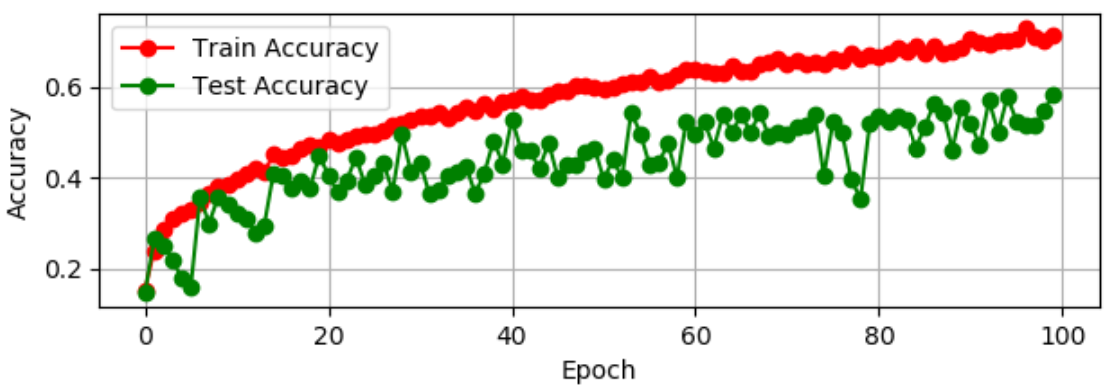
\includegraphics[width=1.0\columnwidth]{Figures/accuracycnnmodel}
\decoRule
\caption[The accuracy of the first convolutional neural network model.]{The accuracy of the first convolutional neural network model.}
\label{fig:cnnaccuracy12}
\end{figure}

Figure \ref{fig:cnnaccuracy12} shows the accuracy of the CNN model across the training and test set. The model was trained on the training data for 100 epochs. The weights of the model which gave the test performance on the validation data were loaded. The model was then tested on the test data. After training the model gave an accuracy of approximately 64.76\% on the training set, while it achieved an accuracy of 60\% on the validation set.


\begin{figure}[ht]
\centering
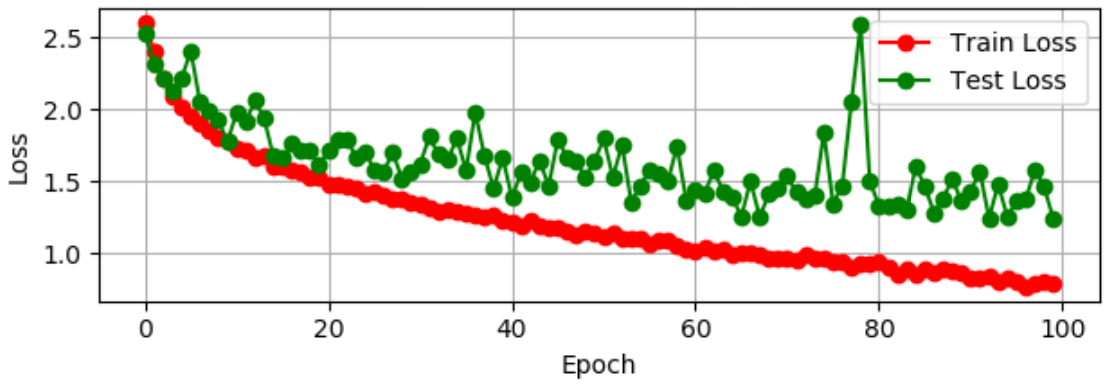
\includegraphics[width=1.0\columnwidth]{Figures/losscnnmodel}
\decoRule
\caption[A visualization of the Loss of the first convolutional neural network model.]{A visualization of the Loss of the first convolutional neural network model.}
\label{fig:cnnaccuracy13}
\end{figure}

Figure \ref{fig:cnnaccuracy13} represents the model loss across the training and test set. These values were calculated according to Equation \ref{eq:lossfunction} above. The results shows that the model achieved a loss of 0.823 on the training set and approximately 1.032 on the validation set.\\

As we can observe from the learning curve from Figure \ref{fig:cnnaccuracy12} and Figure \ref{fig:cnnaccuracy13}, the difference in results between train and test set are not significant, although training set performs slightly better. The training accuracy across the test set were not stable specially at the beginning of the training from 0 to the $18^{th}$ epochs and between the $75^{th}$ and $80^{th}$ epochs. Here, it means that although the model performed better on the training data, but its performance on the validation data get degraded. This is because the model is too complex for the data and it starts to memorize the training data. The same pattern appear on the model loss. Both of the training and test set were having nearly same loss, the training set continue decrease steeply. After that, the model shows over-fitting on the validation set between the $75^{th}$ and $80^{th}$, here the loss dramatically increases. At the end of the training  and after the $80^{th}$ epoch, the model shows good loss results.


\begin{figure}[ht]
\centering
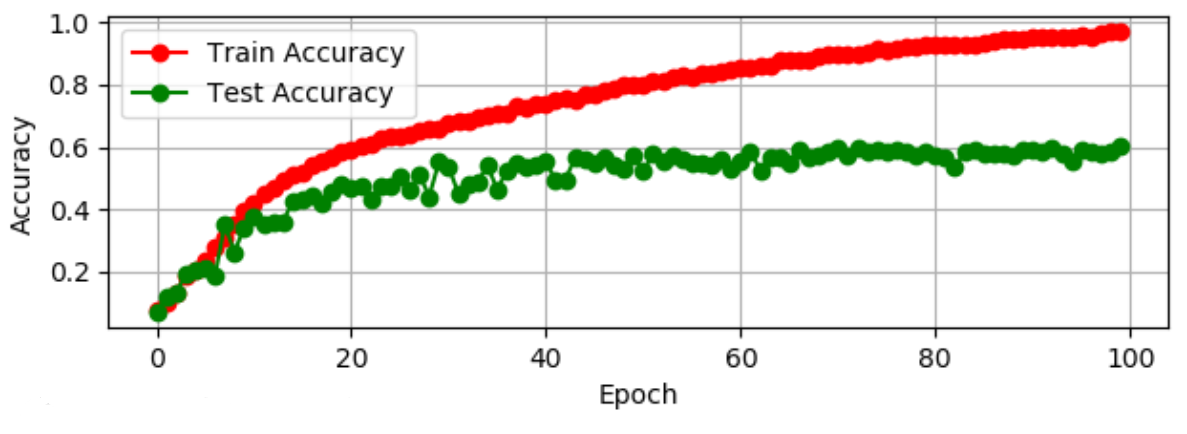
\includegraphics[width=1.0\columnwidth]{Figures/accuracycnnlstmmodel}
\decoRule
\caption[The accuracy of the second convolutional long short term memory neural network model.]{The accuracy of the second convolutional long short term memory neural network model.}
\label{fig:accuracycnnlstmmodel} 
\end{figure}

Figure \ref{fig:accuracycnnlstmmodel} represents the accuracy of the second CNN-LSTM model, which is trained over 100 epochs. In this model the weights that gives the best performance on the validation data were loaded. After that, the model is tested on the test set. At the end of the training, the model gave an accuracy of 92.23\% on the training set and 61.2\% of the test set. The current results are an improvement of 27.47\% from the previous architecture.

\begin{figure}[ht]
\centering
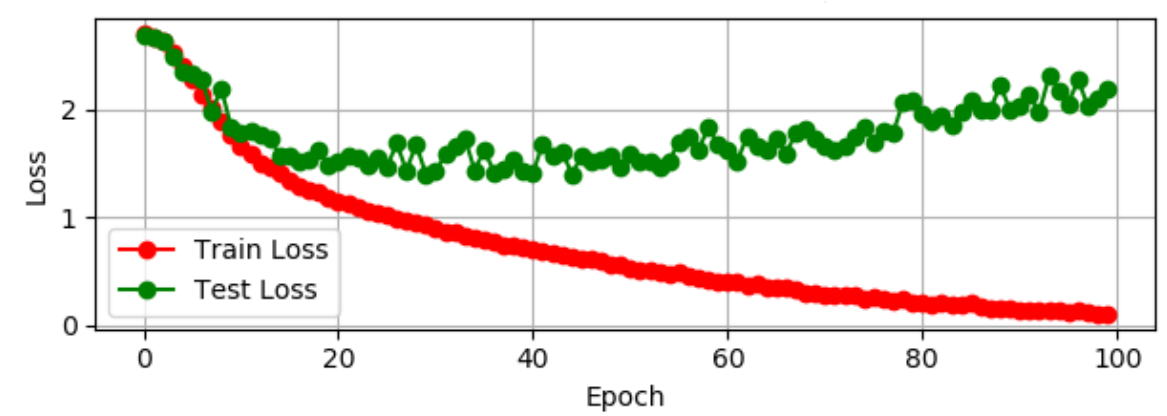
\includegraphics[width=1.0\columnwidth]{Figures/losscnnlstmmodel}
\decoRule
\caption[A visualization of the Loss of the second convolutional long short term memory neural network model.]{A visualization of the Loss of the second convolutional long short term memory neural network model.}
\label{fig:losscnnlstmmodel}
\end{figure}

Figure \ref{fig:losscnnlstmmodel} shows the model loss on the training and test set. This architecture successfully scored a loss of 0.087 on the training set and nearly 2.1 on the test set. This is because the model performed better on the training data, but failed to perform good on the test set, due to the data complexity and variation in the pattern in each frame.\\

As we can observe from the learning curve from figure \ref{fig:accuracycnnlstmmodel} and figure \ref{fig:losscnnlstmmodel}, that the training is more stable than the previous CNN model. However, the model loss did not perform well on the test set, as it shows large differences between the training and test. Overall, final results show that with much deeper model and less parameters, the model is morel likely to perform better and generate more accurate prediction, than a model with less network and more parameters, as it is shown in table \ref{table:finalresults}.
\begin{table}[ht]
\caption{Final results for the CNN and CNN-LSTM model.}
\centering
\begin{tabular}{|c|c|c|c|c|}
\hline
\textbf{Model name} & \textbf{Accuracy} & \textbf{Loss} & \textbf{Layers} & \textbf{Parameters} \\ \hline
\textbf{CNN} & 64.76\% & 0.823 & 13 & 8,543,110 \\ \hline
\textbf{CNN-LSTM} & 92.23\% & 0.087 & 18 & 1,657,792 \\ \hline
\end{tabular}

\label{table:finalresults}
\end{table}\\

%-Confusion matrix----------------------------------------------------------------------------------

Figure \ref{fig:cmsnnlstm}, Figure \ref{fig:cmcnn} and Figure \ref{fig:cmbm} show the confusion matrix of the proposed CNN-LSTM model, the proposed CNN model and the benchmark results released by KTH authors. Technically, the confusion matrix was implemented by randomly selecting 9 different videos from the dataset, then processed these video than consist of different action labels. In this process, all confusion matrix have been converted in the same format, and they have been normalized. We look at the diagonal line in the diagram which shows the accuracy of each particular action labels. In case of Walking, when the actual label was "walking", the benchmark predicted the label 74\% of the time, whereas the proposed models predicted 84\% and 94\% for the CNN and CNN-LSTM respectively. A higher value was scored by the CNN model. In case of Handwaving, when the actual label was "Handwaving", the benchmark predicted the label 55\% of the time, whereas the proposed models predicted 72\% and 74\% for the CNN and CNN-LSTM respectively. A higher value was scored by the CNN-LSTM model. In case of Jogging, when the actual label was "Jogging", the benchmark predicted the label 98\% of the time, whereas the proposed models predicted 69\% and 60\% for the CNN and CNN-LSTM respectively. A higher value was scored by the benchmark model. This suggest that the proposed model was better at predicting jogging action better than the our proposed model. Another interesting pattern appeared in handclapping action, where the proposed CNN model predict this action 100\% all the time, whereas the 60\% of the time for the CNN-LSTM and the benchmark results. That's mean that the model successfully distinguished handclapping from all other activities and had 'no confusion' when giving a prediction about this action. However, for the remaining action like boxing, the CNN model predicted it 14\% and 98\% of the time for the CNN-LSTM model, in this case there are a huge gap between the two models. This means that videos in which action being performed was boxing were predicted by our proposed model with a better recognition rate than that of the benchmark model.\\

Overall, the CNN model scored a high recognition value for "Walking", "Handclapping" and "Running", whereas the CNN-LSTM achieved a high recognition rate for "Handwaving" and "boxing". Both of the model surpassed the benchmark results. In Figure \ref{fig:classified1} and Figure \ref{fig:missclassified1} we present our final prediction on some random frames, we showed the well classified and the miss-classified results. 
\begin{figure}[ht]
\centering
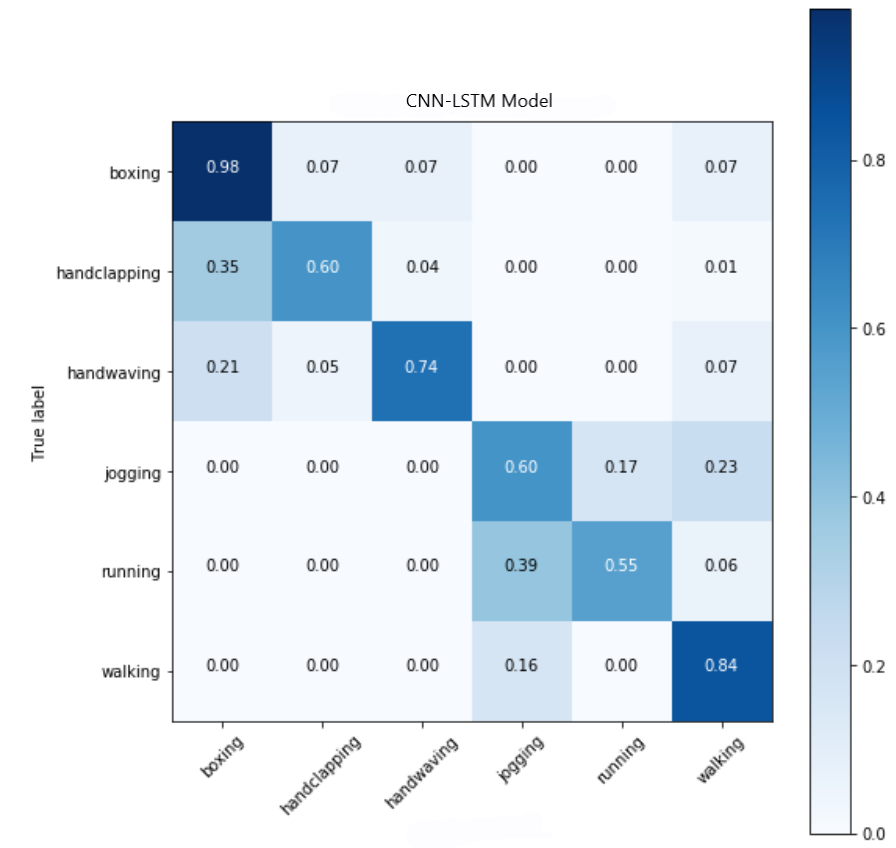
\includegraphics[width=1.0\columnwidth]{Figures/cnnlstmodel.png}
\decoRule
\caption[A visualization of the confusion matrix results for the proposed CNN-LSTM model.]{A visualization of the confusion matrix results for the proposed CNN-LSTM model.}
\label{fig:cmsnnlstm}
\end{figure}


\begin{figure}[ht]
\centering
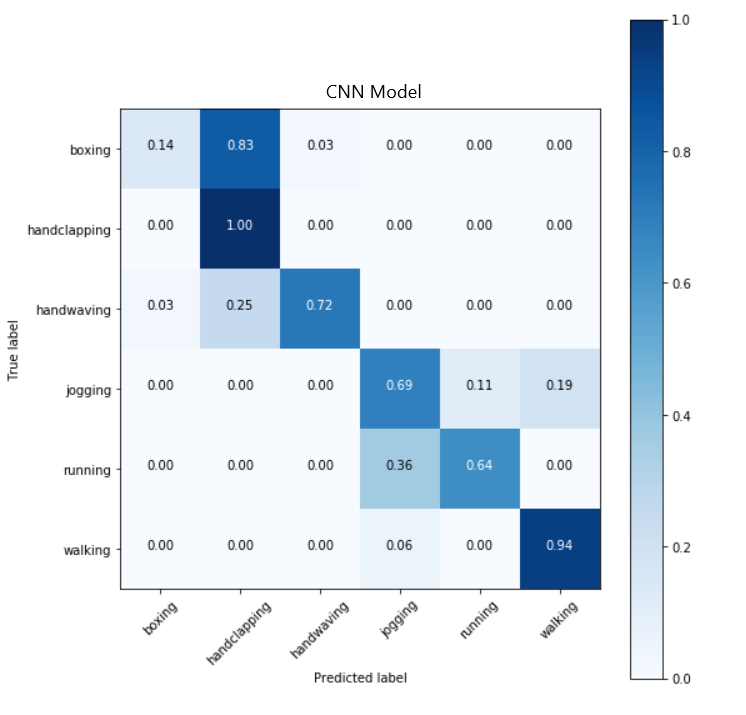
\includegraphics[width=1.0\columnwidth]{Figures/benchmarkresult.png}
\decoRule
\caption[A visualization of the confusion matrix results for the proposed CNN model.]{A visualization of the confusion matrix results for the proposed CNN model.}
\label{fig:cmcnn}
\end{figure}


\begin{figure}[ht]
\centering
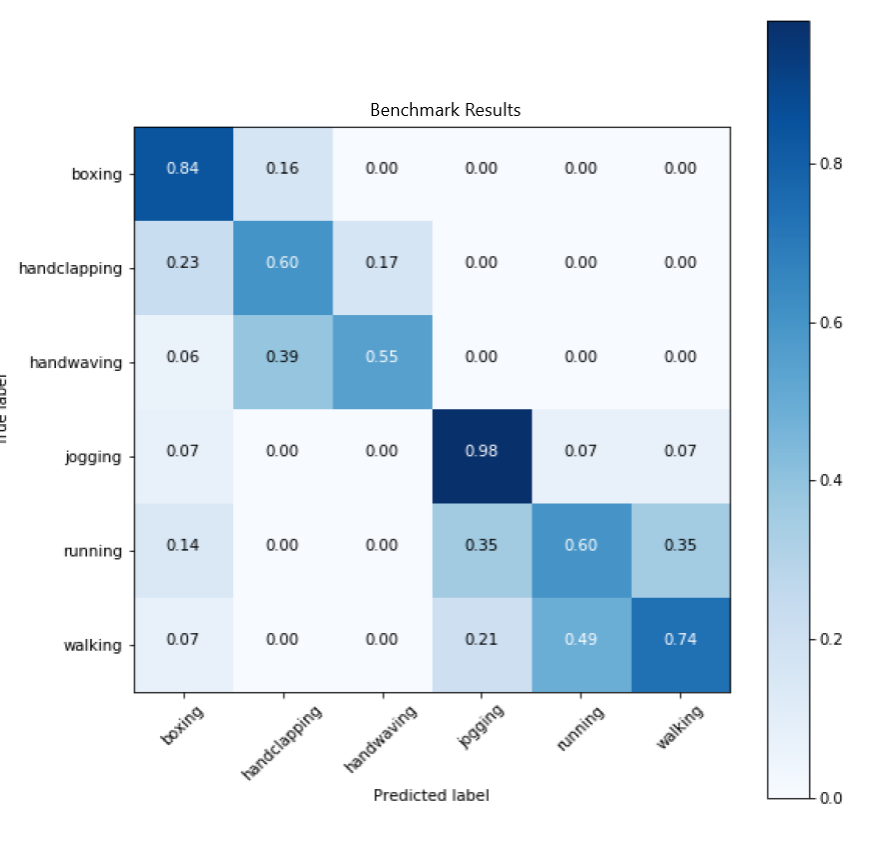
\includegraphics[width=1.0\columnwidth]{Figures/bm.png}
\decoRule
\caption[A visualization of the confusion matrix for benchmark results, released by KTH dataset authors.]{A visualization of the confusion matrix for benchmark results, released by KTH dataset authors.}
\label{fig:cmbm}
\end{figure}

\begin{table}[ht]
\caption{A table represents a summary of the results taken from the confusion matrix.}

\centering
\begin{tabular}{|c|c|c|c|}
\hline
\textbf{Action} & \textbf{CNN model} & \textbf{CNN-LSTM} & \textbf{Benchmark} \\ \hline
\textbf{Walking} & 94\% & 84\% & 74\% \\ \hline
\textbf{Jogging} & 69\% & 60\% & 98\% \\ \hline
\textbf{Handclapping} & 100\% & 60\% & 60\% \\ \hline
\textbf{Handwaving} & 72\% & 74\% & 55\% \\ \hline
\textbf{Running} & 64\% & 55\% & 60\% \\ \hline
\textbf{Boxing} & 14\% & 98\% & 84\% \\ \hline
\end{tabular}
\label{my-label}
\end{table}\\

\begin{table}[]
\caption{We represent the summary of the confusion matrix results.}
\centering
\begin{tabular}{|c|c|c|c|}
\hline
\textbf{Action} & \textbf{CNN model} & \textbf{CNN-LSTM} & \textbf{Benchmark} \\ \hline
\textbf{Walking} & Better & - & - \\ \hline
\textbf{Jogging} & - & - & Better \\ \hline
\textbf{Handclapping} & Better & - & - \\ \hline
\textbf{Handwaving} & - & Better & - \\ \hline
\textbf{Running} & Better & - & - \\ \hline
\textbf{Boxing} & - & Better & - \\ \hline
\end{tabular}

\label{my-label}
\end{table}

\begin{figure}[ht] 
\centering
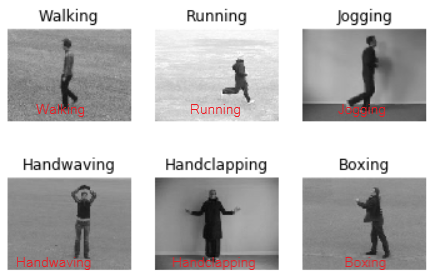
\includegraphics[width=1.0\columnwidth]{Figures/classified.png}
\decoRule
\caption[Visualization of the correctly classified action samples.]{Visualization of the correctly classified action samples.}
\label{fig:classified1}
\end{figure}


\begin{figure}[ht]
\centering
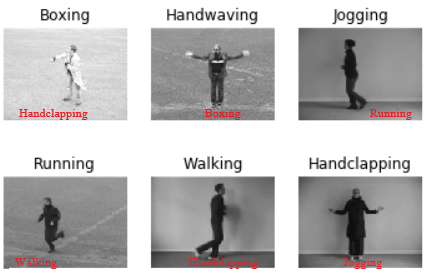
\includegraphics[width=1.0\columnwidth]{Figures/missclassified.png}
\decoRule
\caption[Visualization of the miss classified action samples.]{Visualization of the miss classified action samples.}
\label{fig:missclassified1}
\end{figure}
%----------------------------------------------------------------------------------------
After evaluating our model against the benchmark results, we wanted to know where we stand against other implementations and methods. Therefore, we have conducted an in-depth analysis and collected 29 papers that used the same KTH dataset type and we classified them in term of accuracy and year published and at the end we made a comparison for the same paper that used the same method as us. In Table ~\ref{table:finalresults} we have showed 29 papers; we have showed the authors name, year, method used and the accuracy achieved. Refer to Figure ~\ref{fig:accuracycomparison}, Figure ~\ref{fig:accuracycomparison1} and Figure ~\ref{fig:accuracycomparison2} for visualization. We have highighted our method with red to provide more insight.
%Possible future research directions that could be pursued as a natural extensions of this work are also pointed out.

% Please add the following required packages to your document preamble:
% \usepackage[table,xcdraw]{xcolor}
% If you use beamer only pass "xcolor=table" option, i.e. \documentclass[xcolor=table]{beamer}
% \usepackage{longtable}
% Note: It may be necessary to compile the document several times to get a multi-page table to line up properly
\begin{longtable}[c]{|c|c|c|c|}
\caption{An overview of previous papers and work in the HAR field.}
\label{PreviousResults}\\
\hline
\textbf{Author}                                                  & \textbf{Year}               & \textbf{Method}                                                                                 & \textbf{Accuracy}             \\ \hline
\endhead
%
\textbf{Our Method}                                              & {\color[HTML]{000000} 2019} & {\color[HTML]{000000} \begin{tabular}[c]{@{}c@{}}CNN -\\   RNN network\end{tabular}}            & {\color[HTML]{000000} 92.23\%} \\ \hline
\begin{tabular}[c]{@{}c@{}}\cite{laptev2004recognizing}\end{tabular}      & {\color[HTML]{000000} 2004} & {\color[HTML]{000000} \begin{tabular}[c]{@{}c@{}}Local\\   Feature, SVM\end{tabular}}           & {\color[HTML]{000000} 78\%}    \\ \hline
\begin{tabular}[c]{@{}c@{}}\cite{laptev2004recognizing}\end{tabular}      & 2004                        & Histogram Local Feature                                                                         & 75\%                           \\ \hline
\begin{tabular}[c]{@{}c@{}}\cite{laptev2004recognizing}\end{tabular}      & 2004                        & Histogram STG                                                                                   & 75.50\%                        \\ \hline
\begin{tabular}[c]{@{}c@{}}\cite{laptev2004recognizing}\end{tabular}      & 2004                        & \begin{tabular}[c]{@{}c@{}}Histogram\\   LF\end{tabular}                                        & 70\%                           \\ \hline
\begin{tabular}[c]{@{}c@{}}\cite{laptev2004recognizing}\end{tabular}      & 2004                        & \begin{tabular}[c]{@{}c@{}}Histogram\\   STG\end{tabular}                                       & 67\%                           \\ \hline
\cite{moussa2015enhanced}                                                  & 2015                        & \begin{tabular}[c]{@{}c@{}}SIFT\\   \end{tabular}            & 97.89\%                        \\ \hline
\begin{tabular}[c]{@{}c@{}}\cite{bregonzio2012fusing}\end{tabular}     & 2012                        & \begin{tabular}[c]{@{}c@{}}Feature\\   Fusion\end{tabular}                                      & 94.33\%                        \\ \hline
\begin{tabular}[c]{@{}c@{}}\cite{liu2008learning}\end{tabular}         & 2008                        & \begin{tabular}[c]{@{}c@{}}Bag of\\   video-words\end{tabular}                                  & 94.20\%                        \\ \hline
\begin{tabular}[c]{@{}c@{}}\cite{lin2009recognizing}\end{tabular}           & 2009                        & \begin{tabular}[c]{@{}c@{}}Prototype-based\\   approach\end{tabular}                            & 93.43\%                        \\ \hline
\begin{tabular}[c]{@{}c@{}}\cite{chen2009mosift}\end{tabular}    & 2009                        & MoSIFT                                                                                          & 95.83\%                        \\ \hline
\begin{tabular}[c]{@{}c@{}}\cite{niebles2008unsupervised}\end{tabular}       & 2008                        & \begin{tabular}[c]{@{}c@{}}Spatial-Temporal\\   Words\end{tabular}                              & 95.83\%                        \\ \hline
\begin{tabular}[c]{@{}c@{}}\cite{tran2011modeling}\end{tabular}          & 2011                        & \begin{tabular}[c]{@{}c@{}}Pictorial\\   structures model\end{tabular}                          & 95.67\%                        \\ \hline
\begin{tabular}[c]{@{}c@{}}\cite{fathi2008action}\end{tabular}       & 2008                        & \begin{tabular}[c]{@{}c@{}}Low-level\\   optical flow\end{tabular}                              & 90.50\%                        \\ \hline
\begin{tabular}[c]{@{}c@{}}\cite{kovashka2010learning}\end{tabular} & 2010                        & \begin{tabular}[c]{@{}c@{}}Space-time\\   feature\\ neighborhoods\end{tabular}                    & 94.53\%                        \\ \hline
\begin{tabular}[c]{@{}c@{}}\cite{cao2010cross}\end{tabular}           & 2010                        & \begin{tabular}[c]{@{}c@{}}Maximum\\   a Posterior (MAP)\\  estimation\end{tabular}                & 95.02\%                        \\ \hline
\begin{tabular}[c]{@{}c@{}}\cite{kaaniche2010gesture}\end{tabular} & 2010                        & \begin{tabular}[c]{@{}c@{}}Local\\   motion signatures (LMSs)\end{tabular}                      & 94.67\%                        \\ \hline
\begin{tabular}[c]{@{}c@{}}\cite{dollar2005behavior}\end{tabular}        & 2005                        & \begin{tabular}[c]{@{}c@{}}Spatial\\   and temporall features\end{tabular}                      & 81.17\%                        \\ \hline
\begin{tabular}[c]{@{}c@{}}\cite{klaser2008spatio}\end{tabular}        & 2010                        & \begin{tabular}[c]{@{}c@{}}Histograms\\   of oriented 3D \\ spatio-temporal gradients\end{tabular} & 91.40\%                        \\ \hline
\begin{tabular}[c]{@{}c@{}}\cite{klaser2008spatio}\end{tabular}         & 2008                        & \begin{tabular}[c]{@{}c@{}}Motion\\   Context (MC)\end{tabular}                                 & 91.33\%                        \\ \hline
\begin{tabular}[c]{@{}c@{}}\cite{rodriguez2010spatio}\end{tabular}     & 2010                        & \begin{tabular}[c]{@{}c@{}}Maximum\\   average\\     correlation height\\  filter\end{tabular}     & 80.90\%                        \\ \hline
\begin{tabular}[c]{@{}c@{}}\cite{ke2005efficient}\end{tabular}            & 2005                        & Adaboost                                                                                        & 62.97\%                        \\ \hline
\begin{tabular}[c]{@{}c@{}}\cite{laptev2008learning}\end{tabular}        & 2008                        & Support Vector Machine - SVM                                                                    & 91.80\%                        \\ \hline
\begin{tabular}[c]{@{}c@{}}\cite{wang2011action}\end{tabular}          & 2011                        & \begin{tabular}[c]{@{}c@{}}Dense\\   trajectory\\  with HOG, HOF, MBH\end{tabular}                 & 94.20\%                        \\ \hline
\begin{tabular}[c]{@{}c@{}}\cite{wang2011action}\end{tabular}          & 2012                        & \begin{tabular}[c]{@{}c@{}}STIP\\   with HOG, HOF\end{tabular}                                  & 92.13\%                        \\ \hline
\begin{tabular}[c]{@{}c@{}}\cite{grushin2013robust}\end{tabular}       & 2013                        & RNN with  LSTM                                                                                  & 90.70\% \\ \hline
\begin{tabular}[c]{@{}c@{}}\cite{wang2011action}\end{tabular}          & 2015                        & \begin{tabular}[c]{@{}c@{}}Differential\\   Recurrent Neural\\  Network (dRNN)\end{tabular}        & 93.96\% \\ \hline
\begin{tabular}[c]{@{}c@{}}\cite{zhen2016action}\end{tabular}          & 2016                        & \begin{tabular}[c]{@{}c@{}}STIP\\   with HOG3D\end{tabular}                                     & 94.10\%                        \\ \hline
\begin{tabular}[c]{@{}c@{}}\cite{shi2017sequential}\end{tabular}           & 2016                        & RNN and Deep ConvNets                                                                           & 96.80\%                        \\ \hline
\end{longtable}



\begin{figure}[ht]
\centering

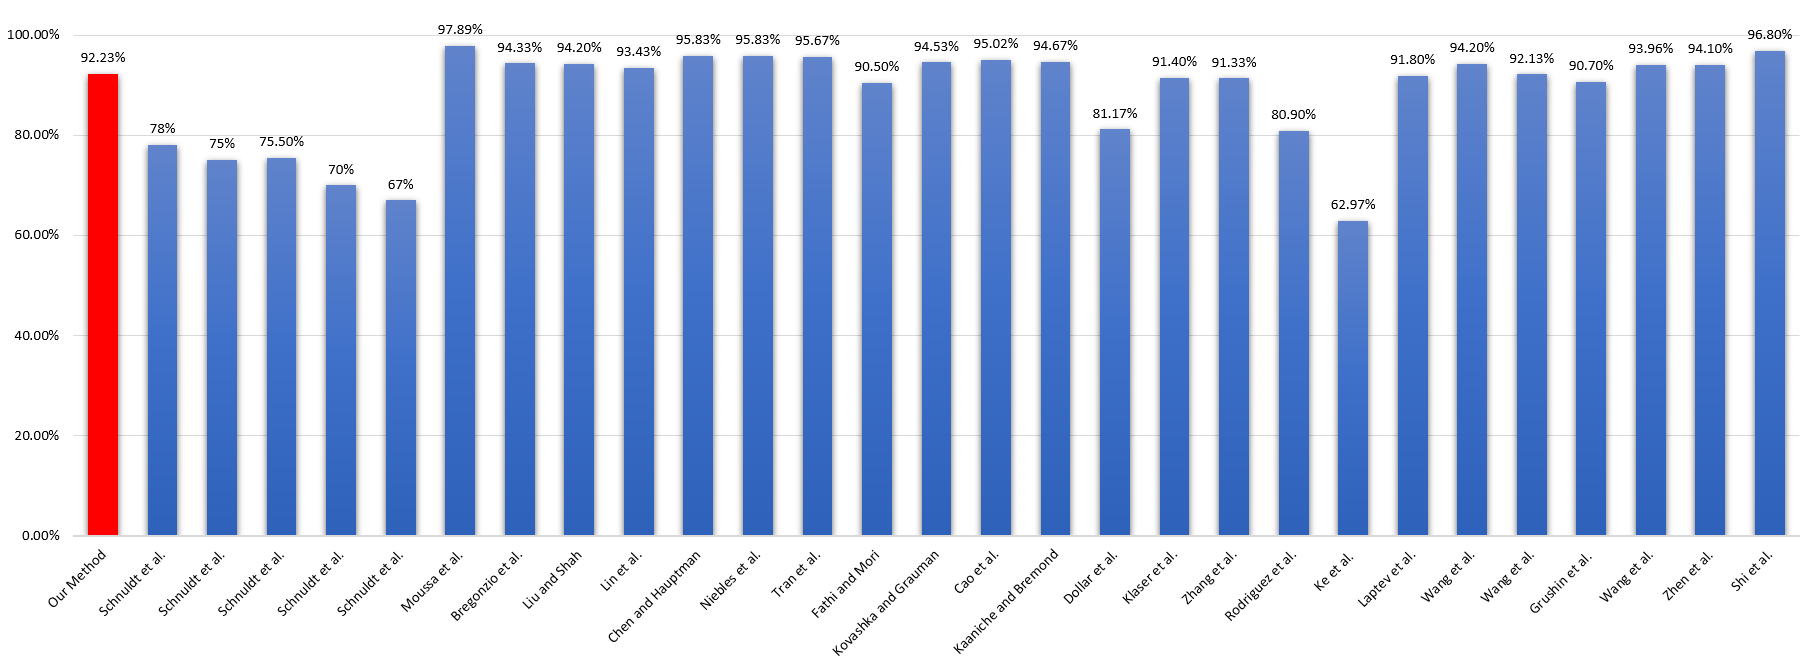
\includegraphics[angle=90,origin=c,width=0.6\columnwidth]{Chapters/photos/comparisonintermofaccuracy.PNG}

\decoRule
\caption[A comparison of our method against other papers in term of accuracy.]{A comparison of our method against other papers in term of accuracy.}
\label{fig:accuracycomparison}
\end{figure}



\begin{figure}[ht]
\centering
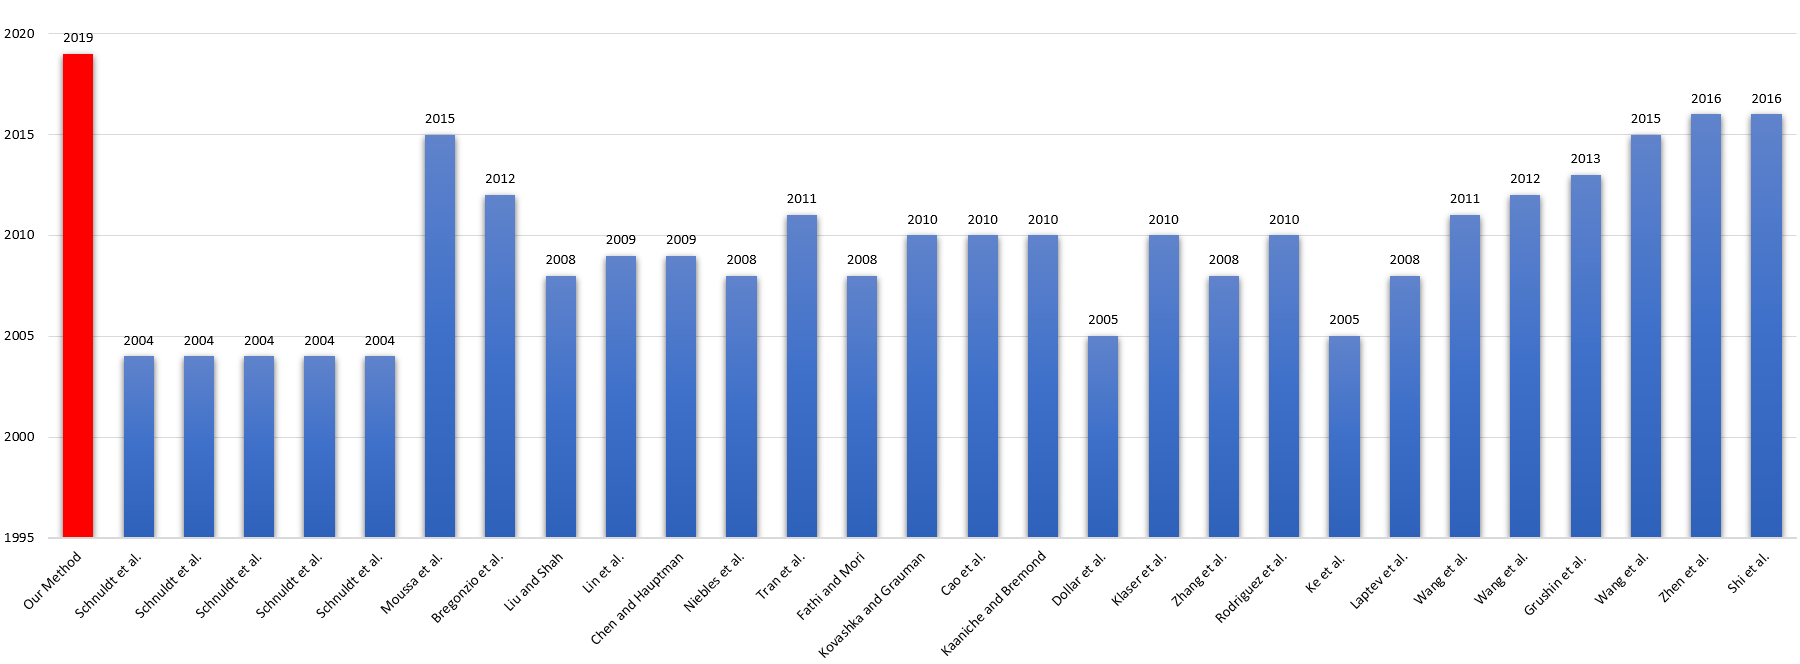
\includegraphics[angle=90,origin=c,width=0.6\columnwidth]{Chapters/photos/comparisonintermofyear.PNG}
\decoRule
\caption[A comparison of our method against other papers in term of year published.]{ comparison of our method against other papers in term of year published.}
\label{fig:accuracycomparison1}
\end{figure}

\begin{figure}[ht]
\centering
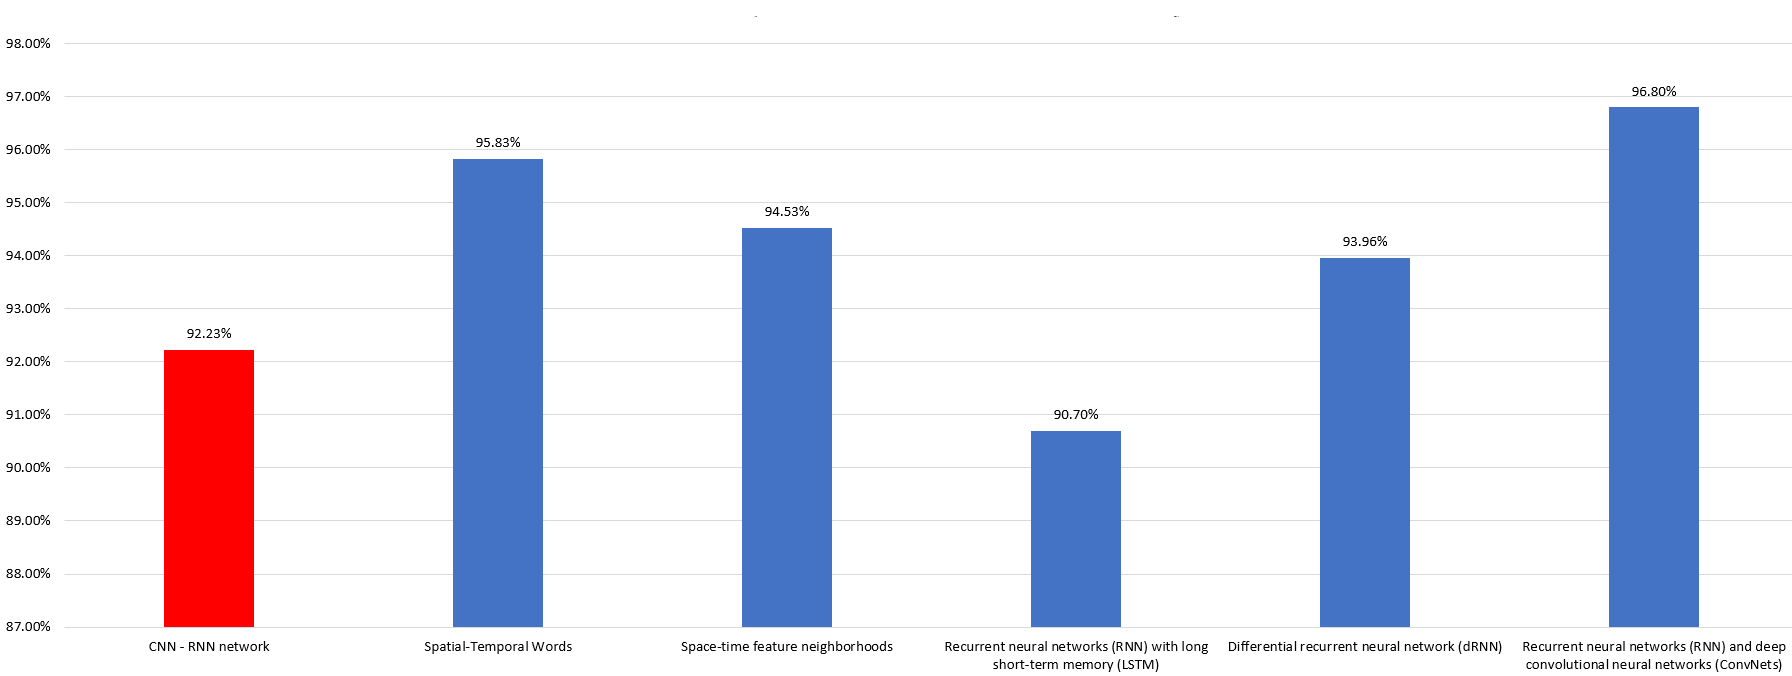
\includegraphics[angle=90,origin=c,width=0.6\columnwidth]{Chapters/photos/comparisonintermofCNNRNN.PNG}
\decoRule
\caption[A comparison of our method against other papers in term of method.]{ comparison of our method against other papers in term of method.}
\label{fig:accuracycomparison2}
\end{figure}
\section{Summary}
In this chapter we represent our network performance. We proposed 2 methods: a method that encodes spatial information using CNN layers and regularization and a method that encode the same information with an additional memory architecture added to the model, where spatial and temporal features are concatenated and trained to predict the label of a particular sequence.
The CNN takes advantage of implicit posture information and it is able to efficiently encode spatial information. While the other model predict the action based on a sequence of frame using recurrent gates.
Final experimental results shows that the proposed models surpassed benchmark results significantly. The CNN model was able to recognize three action higher than any other model, while the CNN-LSTM was able to score a high value for two actions.

Finally we would like to highlight that propose spatial layout encoding methods improve both hand-crafted and CNN based representation and lead to significant improvements in recognition accuracy.
%----------------------------------------------------------------------------------------

\chapter{Conclusion and Recommendations}

This chapter presents a summary of the work presented in this thesis and the conclusions drawn from it, and a brief conclusion of research gaps, research objectives, the methods used and their obtained results. Even though several activity recognition frameworks exist in the previous literature, memory-based systems are very popular due to their simplicity and their superior performance. In this thesis, feature-based and memory-based action recognition has been extensively studied and several advances have been proposed. The summary follows the three main research themes and areas of contribution in providing a comprehensive evaluation of the feature-based action recognition system, improving the system performance by developing new, efficient spatio-temporal features and developing new feature representation and classification architecture to improve the overall recognition performance amongst benchmarks. Possible future research directions that could be pursued as a natural extensions of this work are also pointed out. 

\section{Limitations and Research gaps}
The methods proposed in this thesis have still some limitations. Some of them can be seen
as extensions and can be solved in near future. While others are still open questions. In this section we present the limitations and research gaps.\\

The method proposed and the data used in this thesis assumes that there is only one person in the scene. In real-world scenarios, more people might be present on the scene. In particular some action involves more than one person,  this case is not covered by the proposed method. Modeling spatial layout that only rely on people appearance may not work when actions are done by multiple humans, where multiple actions are performed by many people that looks the same. In addition our Mixture of CNN and RNN concentrates too much on areas with high action of interest, which limits it’s performance in real world scenario.\\

Unconstrained action recognition from “real-world” videos,
however, remains a challenging problem. State-of-the-art
methods are currently very far from the perfect scores obtained by systems developed for image classification due to activity complexity, insufficient training set and personal biometric signature. This fact is underscored by the properties of the benchmarks
used to develop, train, and test systems for action recognition in videos, compared to systems for image classification, where the latter include hundreds of action categories and labels,
peaking at thousands of video samples, the former provide
thousands of categories and millions of photo samples. This
is particularly troubling when considering that actions can
vary greatly in how they appear in videos, and that most of the people appear to perform action that is even confusing to be recognized by human, possibly far more
than static items vary in appearance in photos, implying that
data sets for action recognition must be designed to offer
more examples and cover many scenarios with less computation power.

\section{Future Work}
This thesis contribute to the field of human action recognition. Given these contribution, it is important that the works continues to improve and develop to provide further applications in human activity recognition and advance the field of computer vision further.\\

It is suggested that the feature-based CNN methodology introduced in Chapter 2, could be improved by removing the limitation of number of frames selected per activity. This would allow activities that have more motion present to have more features while activities with fewer movements can be represented by fewer features. A second suggestion could be to adopt a bounding box based approach by modelling the features
inside a particular box for each region in the frame. This could prove useful to provide a better model of more localised activities.\\

The second activity recognition approach introduced in the same Chapter could be improved by adding the tracking approach. The action can be then detected more robustly and the long term changes in motion and location would also be modelled. A further suggestion is to modify the proposed concatenation methodology either by using a depth estimation to determine the approximate distance of the pedestrians from the camera, or by fusing the CNN model and LSTM with Generative adversarial network (GAN) that generator predict action labels and the discriminator distinguish between the real prediction and the fake one. The performance can also be improved by introducing attentions mechanism to the network, we believe that long, complex action recognition or action detection can be improved with attention mechanism. Such mechanism lets the algorithm focus on important subsequences of action.\\

Finally, I suggested to adopt the bounding box approach for both of the methods introduced in Chapter 2. This method is intended to focus on the human as object of interest and the proposed model is applied to down sample the video before being fed to the neural network then automatically predict its associated labels. I also plan to use Depth sensor to introduce the depth as a new set of information; this information will allow the system to learn more about the video, and therefore, produce more accurate results. 

\section{Conclusion}
This thesis proposed and examined two deep neural network architectures and proved that they can be used for human action recognition in video sequences. The widely know AlexNet CNN architecture was intensified with different regularization layers to improve action predictions that make use of several frames of video for their recognition. The motivation is that when a single-frame feedforward neural network is used to distinguish actions in videos the resulting actions trajectory is noisy and requires postprocessing. A recurrent neural network can learn to track activity across multiple frames as a result of the learning and produce smoother detections. A convolutional multiple-frame action detector neural network acted as a baseline model for all comparisons.\\

The experiments measured the models’ performance under varying levels of scenarios applied to the videos dataset such as zooming, light effect, outdoor and indoor etc. The results showed that the recurrent architectures outperform the CNN action detector model and are more robust to variation and noise. The models are also more confident in their predictions. The recurrent architectures also defeat and outperform the benchmark model in action detection tasks as they form a temporal context across several frames of video.\\

A set of recurrent models was examined and it is likely that the choices of learning rate, activation functions, kernel sizes, layer count, etc. were not optimal for this problem. The interactions between hyper-parameters can be difficult to predict and the difficulty increases with every distinct hyper-parameter. Finding the optimal architecture and parametrization for this problem was left for future research. Neural networks are complex nonlinear models and creating them requires an instinctive high-level understanding of the learning dynamics. This thesis gave some practical insights into choosing the network structure, learning rate and other hyper-parameters. However, the field of deep learning is developing rapidly and more concrete guidelines for neural network design are apparent to arrive in the future. In the end, it is noteworthy that the experimenter evaluates many models suitable for their particular problem.\\




\chapter{Project Timeline}

\begin{figure}[ht]
\centering

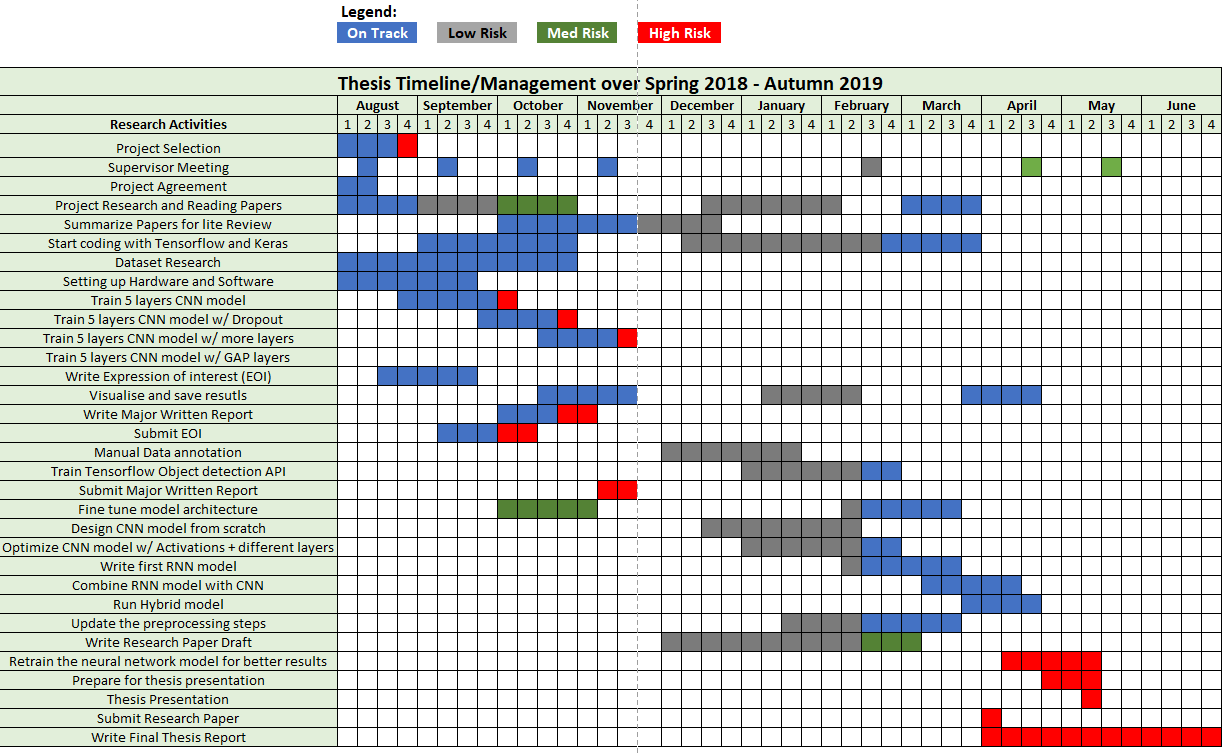
\includegraphics[angle=90,origin=c,width=0.7\columnwidth]{Figures/Project_Timeline.PNG}
\decoRule
\caption[Engineering Thesis 1 \& 2 Gantt Chart: Illustrate the tasks performed between Spring 2018 - Autumn 2019.]{Engineering Thesis 1 \& 2 Gantt Chart: Illustrate the tasks performed between Spring 2018 - Autumn 2019.}
\label{fig:missclassified1}
\end{figure}

\chapter{Appendices}
In the appendices, we have included the Introduction, Literature Review, Methodology, Results and Conclusion from last Thesis submission. We also presented the code used in building the neural network architecture and the building blocks for the data pre-processing pipeline.


\section{Abstract}
\hspace{5mm} Autonomous action recognition is important as it is enabling the creation of various useful applications such as surveillance system, personal assistants, patient monitoring, kinesiology[1] and vision based human computer interaction (HCI). The current systems are not able to achieve an accurate and continuous recognition due to large amount of data in human activity and the computational cost needed for such an application.\\

In this thesis, we propose and validate a method to recognize human actions from a set of video sequences. The aim is to contribute to the recent advancement in this field and develop a deep neural network (DNN) that utilizes the appearance information for each frame to correctly label human actions within a short period of time. To achieve this, research questions are formed to study a live recognition system via directly detecting action instances from untrimmed videos, and to address the issue of adding anomalies to reduce the system confusion in a noisy environment, and to study the feature fusion for multi camera frames to ensure providing a consistent situational context. The method systematically derives spatial and temporal vectors from a sequence of videos and feed these vectors to a convolutional neural network (CNN) model with 9 layers that learn all the possible features from each frame.\\

Preliminary results show that, the proposed model has the capabilities of classifying up to 6 actions categories and able to achieve as high as 69.3\% of recognition rate using the challenging and well studied KTH dataset.


\section{Introduction} % Main chapter title
In this chapter, we introduce the topic of this thesis. First, we present the research motivation of our work and its related applications (section 1.1). Then, we describe the main research challenges related to human action recognition (HAR) (section 1.2), and we present our main research objectives (section 1.3). Finally, we finish this chapter with the thesis structure and outline (section 1.4).
\label{Chapter1} % For referencing the chapter elsewhere, use \ref{Chapter1}


\section{Research Motivation}
\hspace{5mm} HAR is one of the most interesting research topics in computer vision and deep learning. Moving from 2D image to 3D spatial temporal image sequence makes the recognition greatly complex and challenging. It also provides a wide space for various attempts to solve many problems. The goal is to automatically detect the type of action performed in the scene. To achieve this, a video is segmented to contain one execution of action.\\

The execution of HAR became possible with the rise of more powerful hardware and software. Therefore, new types of human actions recognition are now being enabled depending on the category of an activity under consideration. Generally, They are divided into four categories, i.e, gestures, actions, interactions and group activities. The division made is mainly based on the action complexity and its duration [2]. 
\begin{figure}[th]
\centering
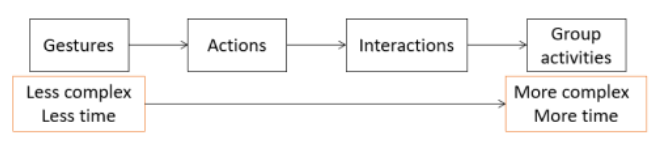
\includegraphics{Figures/mh.PNG}
\decoRule
\caption[Types of Human Action Recognition "HAR"]{Types of Human Action Recognition (HAR).}
\label{fig:la}
\end{figure}\\

\textbf{Gestures:} They are the single body parts movement, which carry some meaning and usually performing a gesture takes short amount of time and it is less complex among the mentioned categories. Hand shaking and facial expressions are good examples of gestures.\\

\textbf{Actions:} They represent combinations of multiple gestures that happen in a short period of time and performed by a single person. Some examples of actions are walking, jogging, running.\\

\textbf{Interactions:} They are the action performed by two actors in the scenes. The Interaction could be between human and human or human and object. For example, a person is riding a bike, is an example of human-object interaction, while two people are fighting is an example of human-human interaction.\\

\textbf{Group activities:} It is formed jointly by groups of people or object or both. It involves combination of gestures, actions and interactions. People are walking in a shopping center is a good example of group interactions that present number of people doing the same actions.\\

As the title suggest, this thesis consider gestures and actions for solving the recognition problem. Therefore, the recognition of interactions and group activities are not covered under the thesis scope.\\

In recent years, HAR has drawn much attention of researchers and scientists worldwide due to its important application in the real world scenarios. This is a great motivation factor for this thesis. There are various applications for HAR including, but not limited to the following:\\
\begin{itemize}
\item \textbf{Human Behavioral Understanding} - This technique is  using statistical models, to analyze the detected pattern in everyday's scenario. For example, self-driving car track driving behaviors and their reaction in different scenario to understand how human naturally behave.
\item \textbf{Video Indexing and Retrieval}- An application that help in automate content retrieval from News and Sport, where videos archives are categorized based on their context. An example of this application, is navigating through contents and rewind the next goal in a soccer match.
\item \textbf{Human Computer Interaction (HCI)} - As technology is moving toward IOT (Internet of Things) and Robotics Automation System (RAS). Activity recognition is being used for controlling home entertainment systems by understanding the human gesture. An example of such a type of interface used for controlling the presentation slides using hand movement [3].
\item \textbf{Human-Robot Interaction (HRI)} - An application that give the robot to ability to recognize human activities is useful for the industrial setup and the domestic environment. For example, a humanoid robot in a domestic environment can recognize human a set of image sequence [4]. 
\item \textbf{Smart Video Surveillance} - Unlike the conventional security surveillance which require laborious human monitoring for content analysis. A smart video surveillance systems aim to automatically track the person or the crowd and recognize the executed action. For example, detecting suspicious activities and create an automatic alert for immediate reporting to the authority [5]. This application will reduce the workload of the security person, and prevent dangerous situation.
\item \textbf{Ambient assisted living (AAL)} - This type of application is used in health care and hospital to understand patient activities and behaviours. Such application can facilitate health treatment, diagnosis, and general patient health care. This system is also used to monitor the daily life of elderly people by capturing their continuous movements.
\item \textbf{Autonomous driving system} - This HAR techniques act as personnel assistant that are used in recognizing the secondary tasks performed by the driver, such as, answering the phone, while operating the vehicle which can prevent a serious accident.  
\end{itemize}

\section{Research Challenges}
\hspace{5mm} Action recognition can be applied at different types of abstraction. Over the last three decades, many approaches were proposed to define these levels of abstraction. The main target in this Thesis is to address the issue of automatic HAR via supervised learning, which mean that there are enough data annotation and labeling for every video and actions. The model is then trained to recognize these actions for unseen videos. The model can be trained on different types of video, such as surveillance videos data or movies data, etc.
\begin{figure}[ht]
\centering
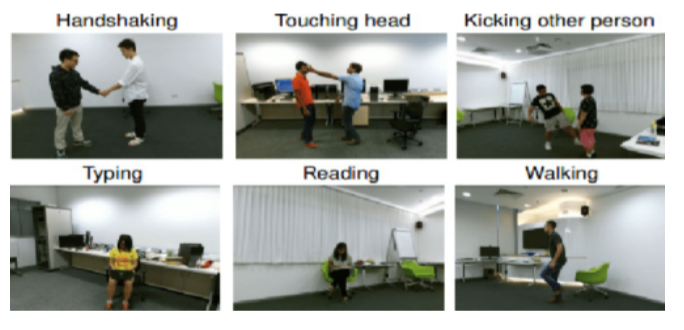
\includegraphics{Figures/ti.PNG}
\decoRule
\caption[Some actions classes in an indoor environment "6"]{Some actions classes in an indoor environment [6].}
\label{fig:la}
\end{figure}
Due to the complexity and large amount of data in humans’ activity, HAR still a challenging task. For example, some of the major challenges are:
\begin{itemize}
\item \textbf{Intra-class and Inter-class variation} - people see and understand actions in many different ways. Also, people move and perform actions in many different ways. For a given action such as “Jogging” and “Running”, the similarity between these two actions is high enough to create confusion for the system. As a result, a model of HAR should be general enough to handle all possible cases of a specific activity as well as discriminative enough to be able to differentiate between types of activities.
\item \textbf{Video Artifacts} - when building a model, the first step is always by preprocessing the data. Depending on the data size, preprocessing requires compressing the data, to process each video frame. As a result, when the video is compressed, noise and artifacts start to appear in the video. However, after many research attempts and judging from old and new results, video artifacts do not always present threat to the model accuracy, specially the existing of many low-resolution methods that works on smoothing the area of the actions with spatial-temporal features. On the other side, noisy video presents an issue for many systems such as indoor/outdoor monitoring, day/night monitoring, which is already low in specific time.
\item \textbf{Dynamic and Cluttered Background} - the practical example of HAR is present it in an outdoor area, where humans are usually not alone the scenes. For example, a scene from an outdoor camera surveillance system or a hospital monitoring system, show humans surrounded by objects and other humans in a dynamic environment, which make the system accuracy and consistency hard to distinguish and localize action for a specific person in a scene.
\item \textbf{Lighting and Hardware Resolution} - this issue exist in outdoor and indoor camera surveillance system, where lighting and distortion create a major problem in the scene. For example, a scene in an indoor environment is always accurate than the outdoor one, due to illumination properties.
\item \textbf{Camera Motion} - in a real-world scenario, a camera mounted to a static pole, suffer from vibration in a windy environment. Another example, exists when recording is done by human hand like “GoPro” and “Phone Camera”, due to zooming or shaking. Even though, some advanced technique tries to stabilize the vibration and clean the data before processing, these algorithms cannot be 100\% accurate, and can affect the HAR [7].
\item \textbf{Variation of Viewpoint} - monitoring large area like “Schools”, “Public Park” etc. Requires multiple cameras around the same environment for better monitoring. However, this will visualize the area from different viewpoint and may cause confusion to the model, which make the system not able to understand the interaction between the human the environment and objects.
\end{itemize}

\section{Research Objective and Scope}
\hspace{5mm} The main objective of this thesis is to improve the performance of video based HAR by proposing a model using handcrafted and deep learning based techniques. This section enlists details objectives of this thesis as follows:
\begin{itemize}
    \item Our first objective is to comprehensively review of novel techniques based on deep learning approaches, in order to decide which video representation method works the best;
    \item Our second objective is to understand the existing limitations of this application and to propose a method that go beyond the state of the art limitations.
    \item Our third objective is to develop a method for spatial temporal feature extraction to make the system understand the visual content in each video frame;
    \item Our fourth objective is to make a comparison between the benchmark and experiment results on the same dataset;
\end{itemize}

\section{Thesis Structure}
\hspace{5mm} This Thesis consists of 7 chapters including the current introductory chapter. They are being organized as following:\\
\begin{itemize}
\item \textbf{Chapter 2} introduces various methods, different features extraction, representation, and classification techniques used by researchers. Also, a review on some of the popular datasets, including the one used for this thesis. A detail review on convolutional neural network for spatial temporal features is also addressed, which is the main focus of this thesis, and justification for the selection is also presented. Finally, contains the research questions to be investigated in the thesis.
\item \textbf{Chapter 3} present a detailed explanation of the proposed model used for this thesis. The methodology includes the software used, the dataset source following with the main implementation.
\item \textbf{Chapter 4} presents preliminary results of the proposed model. We present the evaluation metrics used followed by visualization of results .
\item \textbf{Chapter 5} provides the followed steps to perform all the calculation needed, followed by addressing future plan. 
\item \textbf{Chapter 6} provides detailed schedule with all research activities. The time-line is highly realistic which allows for some degree of flexibility.
\item \textbf{Chapter 7} provides all the references such as, academic journals, publications, PhD dissertation, master dissertation and bachelor thesis.
\end{itemize}

\section{Literature Review}


\subsection{Introduction}
\hspace{5mm} This chapter provides a comprehensive literature review of HAR from video sequences. First of all, the research area of HAR is discussed on a high level, including an overview of neural network types and structure with their conventional training and testing method. Then an in-depth review of the current literature which provide a discussion about state-of-the-art method with respect to their strengths and weaknesses. Toward the end of the literature review, we gave a detailed review on some of the new approaches used that made HAR more accessible and successful.

\subsection{Overview of Neural Networks}
\hspace{5mm} Neural network is a specific kind of deep learning. To understand neural network well, this section provides a detailed explanation of the most popular neural networks that are applied throughout the rest of the thesis. We begin with a brief explanation of multi-layers neural network, convolutional neural network, recurrent neural network, and the popular generative adversarial networks including their type of learning and architecture and provide a visualzation of their networks. Then we explain their training and testing methods.
\subsection{Multi-layers Neural Networks}
\hspace{5mm} Neural networks are a generic term in deep Learning [8] that operate on the basis of the structure and have similar functionality to the human brain. The human brain naturally contains interconnected neurons that transmit signals and data constantly, an artificial neural network has their own interconnected artificial neurons that transmit data between neurons, and same as the human brain operate. The typical neural network consists of 3 layers - input layer, hidden layer and output layer. Technically, inputs data can be any type such as Image, Text, Audio, Video, etc. Hidden layers transform the inputs and perform calculations depending on the system architecture and extract features upon it. The output layer produces the desired output. Each node in the network have a random weight and each layer have an additional bias neuron attached to it to allow shifting the activation function to the left or right which may be critical for a successful learning. Then certain activation functions (Tanh, RELU, Sigmoid, SoftMax etc.) are initialized in the model to make each layer decide which neuron to fire.\\
Neural networks take image as input. The networks flatten them into a 1-D array and this array is given as input to the next neuron. The issue is the spatial features of the pixels and their position in their 2D form is not considered. To illustrate that, suppose there is an image with 256 x 256 pixels, the input is consisting of 65,536nodes, one node for each pixel in the 2D image. The primary disadvantage of this model is that the input vector will be extremely large when dealing with large scale datasets, which make the weight matrix large and make the model computationally expensive. At the end, the network would not be able to give any accuracy. The image below visualize the conventional neural network architecture 
\begin{figure}[ht]
\centering
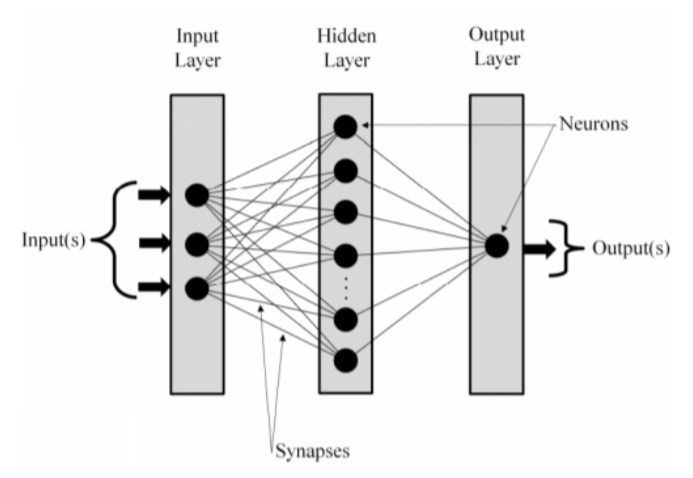
\includegraphics{Figures/ca}
\decoRule
\caption[A visualization of the conventional neural networks architecture "8"]{A visualization of the conventional neural networks architecture [8].}
\label{fig:la}
\end{figure}
\subsection{Convolutional Neural Networks}
\hspace{5mm} Convolutional neural networks are a type of a feed-forward network and they are very similar to the ordinary neural networks but their architecture is designed to process visual features which make the calculation simpler and more optimized. Convolution is the core operation for every CNN operation. The traditional CNN is consisting of 3 layers, for example, Convolution layer, RELU layer, pooling layer and Fully Connected layer. A CNN take as input to the network an arrays of pixel values [9].\\

A convolutional network is dividing images into regions, and then each region is assigned to different hidden nodes. Each hidden neuron in the hidden layer retrieve pattern in only one of the regions in the input image. Each region is called a Kernel or filter. Every filter is convolved over both x-axis and y-axis. Then multiple filter is used to extract different features from the image. A feature map is formed when the output of one filter convolve throughout the entire image generating a 2D layer of neurons. In this case, each filter is responsible of building one feature map.\\

Stacking feature maps can form a 3D array, which can be used as input for the next layer. This is performed by the Convolutional layer. It uses a filter matrix over an array of image pixels and perform the convolution operation to form a convolved feature map. The next layer is the RELU layer, which apply a non-saturating activation function f(x) = max(0,x)and represent the non-linearity to the networks. RELU layer will set all negative pixels to zero and apply an element wise operation. The original image is being scanned by a sliding window in multiple Convolution and RELU layers for locating hidden patterns and features in the image. The output is then a Rectified Feature Map. Other types of activation functions are used in CNN to increase the nonlinearity of the overall architecture. However, RELU is used commonly in CNN models because it led to a faster training without significant loss of accuracy. These layers are followed by a Pooling layer that work on reducing the spatial dimensions of the feature map, generated from the previous convolutional layers. Then the output will be a Pooled feature map. Similarly, to the convolutional layer, pooling layer will scan the image in both the axes and the max value is taken from that filter. The advantage of pooling layer is with reducing the size of the input and the number of parameters and the computational time, which eliminate the problem of overfitting. Finally, the pooling feature map is converted to a long continuous linear vector, which perform the Flatten operation. This flattened matrix generated goes to a fully connected layer to perform a final classification. Fully connected layer is the last layer of the whole architecture, just same as all the other networks.\\

This section covered the implementation of the Convolutional network in case of a 2D images, when a 2D convolutional layers and pooling layers are used. However, for a video setting the implementation become complicated, due to an additional temporal axis. In this case a 3D convolutional layer is used, where the filter of 3 channels is convolved across all the three axes.\\

The main procedure that will be followed to model a CNN is by dividing the entire datasets into 3 parts - training, validation and test set. The model will be trained using the first set of data (training set) repeatedly for a specific number of epochs, also known as iteration. After each epoch during training, the model is tested on the validation set. Then the model that perform with maximum accuracy and less root mean square error on the validation set will be loaded and saved as model weight. Finally, the model performance is then evaluated using the test set.

\begin{figure}[ht]
\centering
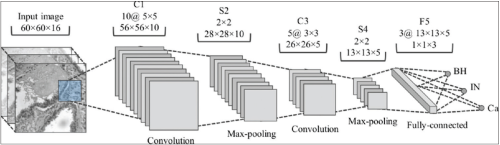
\includegraphics{Figures/cnn}
\decoRule
\caption[A visualization of the convolutional neural networks regular architecture “10”]{A visualization of the convolutional neural networks regular architecture [10].}
\label{fig:la}
\end{figure}
\newpage
\subsubsection{Recurrent Neural Networks}
\hspace{5mm} Recurrent neural networks are a type of network that recognizes patterns from sequence data such as, text, spoken word or time series data [11].\\

RNN is a special network that have a memory to capture information. Theoretically, due to its ability to operate over sequences of vectors, RNN can make use of this information in a long arbitary sequences.\\

RNN is an exciting types of neural network, 
Some examples of the important three design pattern for recurrent networks are below:
\begin{itemize}
    \item Recurrent network linked to the output at every time step, and have recurrent connections between hidden units.
    \item Recurrent network linked to the output at every time step, and have recurrent connections only from the output at one time step to the hidden unit.
    \item Recurrent networks connected with recurrent nodes to the hidden layers, which scan the entire sequence and produce a single output.
\end{itemize} 
However, RNN implementation is not limited to these types, blow are a visualization of the standard RNN architectures used not only on audio, and text data but also on images and videos data:
\begin{figure}[ht]
\centering
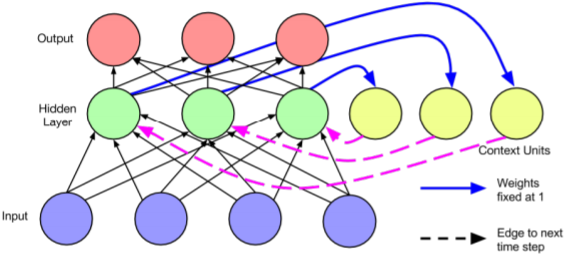
\includegraphics{Figures/rnn}
\decoRule
\caption[A visualization of the recurrent neural networks architectures types"11".]{A visualization of the recurrent neural networks architecture types [11].}
\label{fig:la}
\end{figure}
Each rectangle is a vector and the arrows represent a function such as matrix multiplication, etc. The red arrow is the input  vectors, blue and green arrow hold the RNN state. Model \textbf{(1)} represent a one to one RNN, which process the data from fixed size input to fixed size output and it is used for image classification. Model \textbf{(2)} represent one to many architecture which produce a sequence outputs and its used for image captioning which takes an image and outputs a sequence of words. Model \textbf{(3)} represent many to one which produce a sequence input and it is used for sentiment analysis where the input sentence is classified as positive or negative. Model \textbf{(4)} represents many to many architecture which produce sequence of input and sequence output  and it is used in machine translation, where the RNN take input a sentence in french and output its sentence in english. Model \textbf{(5)} represents another many to many architecture but it synced the input and output sequence, this model is used for video classification where the output is the video label for each frame.\\

\hspace{5mm} Li \textit{et al.} [12] present an adaptive learning framework for skeleton based HAR using RNN-Tree (RNN-T). Their RNN-T model the representation of the human skeleton and recognize them through a hierarchical inference process. The authors address tow main challenges of their large scale recognition model, firstly the ability to classify finer grained actions classes based on confidence rate using single network, secondly, making the model adaptive to new actions and using it in the existing model. The authors prove that their model improve against state of the art methods on many public benchmark.

\subsubsection{Generative Adversarial Networks}
\hspace{5mm} Generative adversarial networks (GAN) introduced by Goodfellow \textit{et al.} [13] are generative model approach based on differentiable generator model. GAN based on a game competition scenario, where the generator network must compete against an adversary and then produce samples directly $x = g(z;\Theta ^{(g)})$. The network adversary or the discriminator network attempts to differentiate between samples drawn from the training and the generator samples. A probability value is then emitted by the discriminator given by $d(x;\Theta ^{^{(g)}})$ as an indicator that the real example from the training example is $x$ rather than a fake sample generated by the model.\\

To describe the learning in the generative adversarial networks is as a zero-sum game, where a function $v(\Theta ^{(g)},\Theta ^{(d)})$ determines the reward of the discriminator. Next the generator receives $-v(\Theta ^{(g)},\Theta ^{(d)})$ as its own reward. As the model learning, each networks try to maximize its own reward following the convergence equation below:
\begin{equation}
    g^{*} = arg\,min{_G}\,\: max{_D}\: v(g,d)
\end{equation}

The objective function of the generator and discriminator is:
\begin{equation}
    min{_G}\,\: max{_D}\: v(g,d) = E{_x\sim {_p{_d}{_a}{_t}{_a}(x)}}[logD(x)] + E{_z\sim {_p}{_z}(z)}[{log(1 - D(G(z)))}]
\end{equation}

\hspace{5mm} The discriminator is then learning to differentiate between the real and fake data. Simultaneously, the generator try to fool the other network into believing that the samples are real. Since an adversarial learning method is applied, the process doesn't require approximating intractable density functions.\\
\begin{figure}[ht]
\centering
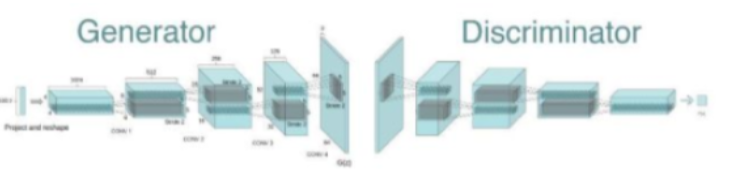
\includegraphics{Figures/gan}
\decoRule
\caption[An visualization for generator and discriminator in GAN networks "14".]{An visualization for generator and discriminator in GAN networks[14].}
\label{fig:la}
\end{figure}
One of the popular example of using GAN is in Auto-encoders and Variational auto-encoders (VAE). Auto-encoders usually encode the input data as set of vectors, and create a compressed representation of the original data. Auto-encoders are used for dimensionality reduction and also paired with a decoder that reconstruct the data based on its hidden layer. An early example of auto-encoders was in Restricted boltzmann machines (RBM) invented by Smolensky [17]. On the other hand, variational auto-encoders are also a generative algorithm that make normalise the hidden layer. VAEs are able to compress acting as an autoencoder and synthesizing data like GAN. However, GAN generate more realistic data with granular details, and the image generated by VAEs are more noisy and blurred.\\
\hspace{5mm} Below is a listed of the current applications of GAN:
\begin{itemize}
    \item Pose Guided person generation[18].
    \item CycleGAN[19].
    \item Re-CycleGAN[20].
    \item PixelDTGAN[21].
    \item Super resolution image resolution[22].
    \item Progressive GAN[23].
    \item StackGAN[24].
\end{itemize}
\hspace{5mm} Kiasari \textit{et al.}[25], proposed an extension on GAN for generating human actions using autoencoders. The authors introduced a model for human action generation in order to generate a sequence of human actions to produce a novel actions. They evaluate their model on the benchmark NTU RGB+D dataset, consisting of 56,880 samples of RGB videos, depth map sequences, 3D skeleton data, and infrared videos for each sample. Their method was able to generate actions with seamless transition with given different labels.
\subsubsection{Training Neural Networks}
\hspace{5mm} The purpose of neural networks is to learn from data. Tom M. Mitchell [26] provides a detailed definition of computer learning:
\begin{displayquote}
"A computer program is said to learn from experience E with respect of some class tasks T and performance measure P, if its performance at tasks in T, as measure by P, improves with experience E".
\end{displayquote}
\hspace{5mm} Different kinds of tasks T, experience E, performance measurements can be used to form and build a machine learning algorithm that can learn.\\
In this case the NN is able to adjust its biases and weights neurons to minimize the training error and on the other hand to maximize the accuracy. Training algorithm are many such as[27]:
\begin{itemize}
    \item Stochastic Gradient Descent.
    \item Back-propagation.
    \item Sparse Training.
    \item Conjugate Gradient.
    \item Adaptive back-propagation.
    \item Genetic algorithm.
    \item Simulated annealing algorithm.
\end{itemize}
\hspace{5mm} Neural networks starts with randomly initializing its weight. During training, the correct class for each reading is known, and the output neurons can be assigned as 1 for the correct value and 0 for the others. Comparing the values calculated from the output nodes through calculating the error in each of the nodes in the network using  the delta rule. The error term is then used to adjust the weight in the hidden layer, which will eventually give better results in the next run.\\

In this thesis gradient descent algorithm is used as traing algorithm. Gradient descent or the delta rule can be written mathematically as the following:
\begin{equation}
\bigtriangledown L \approx \partial \frac{L}{\partial x_{i}}\bigtriangledown x_{i}
\end{equation}


The gradient descent is then being controlled by the learning rate. The rule of updating the weight after each iteration is the following:
\begin{equation}
    W_{j} = W_{j} - lr\partial \frac{L}{\partial W_{j}}
\end{equation}


Where lr is the learning rate and the w is the weight.
\begin{figure}[ht]
\centering
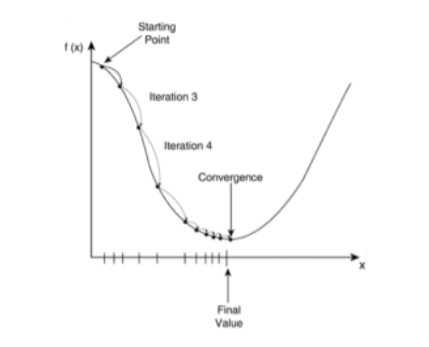
\includegraphics{Figures/lr1}
\decoRule
\caption[Visualization of the gradient descent algorithm during training in a 2D space "41"]{Visualization of the gradient descent algorithm during training in a 2D space [41].}
\label{fig:la1}
\end{figure}

\subsubsection{Testing and fine tuning}
\hspace{5mm} Testing neural networks is a critical final phase of modelling the network. Unlike Training the model, in testing the adjustment of weights and biases values is not required. Testing technique can vary, and one of the interpretation are as the following:
\begin{itemize}
    \item Check up the evaluation matrix weights across epoch.
    \item Removing some of the layers, to observe the variation in the learning process.
    \item Performing Gradient checking. It starts with the activation function derivative, and the total derivative of the cost function to check that there is no error.
    \item Checking the mathematical operation used, especially matrix operation such as the element wise multiplication and the dot product.
    \item create a trivial learning tasks, by letting a single layer to learn the sum of the inputs for the fully connected layer. 
    \item 
\end{itemize}
\hspace{5mm} The second interpretation is by testing the results of the neural network from the hyper-parameters side:
\begin{itemize}
    \item Plotting some metrics such as F1-score, cost, accuracy, amongst train, validation and test set against number of epoch and batch.
    \item Checking gradient vanishing or gradient exploding do not exist in the model. This can be resolved by using different activation function or different learning rate.
\end{itemize}
\hspace{5mm} In this thesis, we consider testing our neural network an essential part of validating our network performance and quality. As a results, a set of validation metrics are introduced in chapter 4. 
\subsection{Holistic Model}
\hspace{5mm} In this section, a comprehensive discussion is covered about features extraction from image sequences. For a robust model, action representation should be rich. These representations are affected by small variations in person appearance, action execution, viewpoint and background. Image representations consider temporal dimension alongside spatial features.\\
\hspace{5mm} Image representations are divided into two main categories:\\
\begin{enumerate}
\item Global Representations.
\item Local Representations.
\end{enumerate}

\subsubsection{Global Representations}
\hspace{5mm} Global representations encode the region of interest (ROI), through background subtraction and tracking. These representations are commonly derived from optical flow, edges and silhouettes. They are also sensitive to variations in viewpoint, partial occlusions and artifacts. To overcome these, a grid-based approaches divide the representations into cells, which encodes part of the observation locally. Overtime, multiple images are stacked to form a three-dimension space-time volume, which create the suitable volume for action recognition.\\ 

The earliest example of silhouettes extraction was introduced by Bobick and Davis [41], which results in a 2D binary MEI as an indication of motion occurrences, by extracting silhouettes from a single view. From the same silhouettes motion, an MHI is raised where pixels are intense due to constant motion overtime. The main purpose of using MHI and MEI, is to overwrite scenario where motion is repeated over the same spatial space. This model is able to detect simple gesture, such as hand waving, hand clapping.   
\begin{figure}[ht]
\centering

\includegraphics{Figures/hg}
\decoRule
\caption[Visualization of motion energy image (MEI), and motion history image (MHI) "42"]{Visualization of motion energy image (MEI), and motion history image (MHI) [42].}
\label{fig:la1}
\end{figure}
MHI suffer from overlapping, a new approach from [43] was proposed. In this method, vertical and horizontal components each with negative and positive directions as four optical flow channels. The purpose is to avoid self-occlusion of the person. These vectors were used in derive kinematics features, such as, symmetry and divergence. A principle components analysis (PCA) is then used to show the main kinematics modes. Due to one disadvantage of silhouette models which present in extracting a robust and accurate silhouette. A new approach was proposed to develop a more practical application for silhouette model by applying Radon transform by [43] where the third dimension is time. R transform has low computational cost and high efficiency in recognizing similar action even silhouette with holes and frame loss data. 


\subsubsection{Local Representations}
\hspace{5mm} Local representations extract features as a collection of patches and local descriptors. Patches are space-time interest points. The differences between the previous representations, is that local representation is not limited to background subtraction and accurate localization. The observation is grouped within a local grid, and finding the correlation between space and time patches. Since the patches are retrained, the action can be modelled effectively.\\

A number of approaches proposed to use representation motivated by HAR. Joint angle and locations considered a rich representation, as it annotated the whole-body key point with specific coordinate system. The advantage of this method is that actions can be analyzed in a more descriptive way. However, it is challenging to derive them from videos. In 2D, there have been number of methods to match 2D joint trajectories with the right action labels. Whereas for 3D, the representations are view-invariant and a reliable low-level joint estimation is required. This is not a issue on a small data with simple human activity, but it is a major problem on large scale data. In a practical real-world application, it is difficult task to develop due to the computational complexity.


\subsection{Human-Object interaction model}
\hspace{5mm} In the case of human interaction, the interaction can be between humans (Human-Human recognition), or between objects and humans. For example, to recognize a human-object interaction, the system needs to recognize and localize the object surrounded by the user, and be aware or its movements [44], same approach apply on human-human interaction. This type of system follows the methodology below:\\

\begin{figure}[ht]
\centering
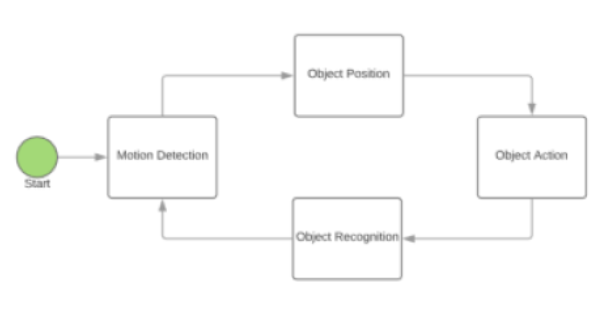
\includegraphics{Figures/ht1}
\decoRule
\caption[Flowchart for an object human activity recognition (HAR) "44"]{Flowchart for an object human activity recognition (HAR) [44]).}
\label{fig:la}
\end{figure}
Ryoo and Aggarwal [45], present a model that can recognize human interactions with objects. As a result, HIR in an airport environment worked on scenario like “A person is stealing baggage”, “A person left baggage on the floor”, by using a complex probabilistic framework that integrate the recognition decision between each existing component. Finally, the object recognition and the motion estimation increases using feedback from the segmented layer. Gupta et al. [46], present a classification approach for understanding human interactions with objects. To classify these activities a Bayesian network is implemented with HAR to discriminate two objects that have same shape but different functionality, such as “Water Bottle” and “Spray Bottle”, using contextual information. These contextual information’s are providing the functional information’s for each object to make the recognition more accurate. In [47], the author developed a framework where the object is recognized first and then the interaction between them is estimated and a HMM is combined with context information to characterize the relationship between actions and objects. Bayesian network is used to label and to classify actions classes, and differentiate unrecognized actions. The approach worked well in different environment evolving one object with one human.

\subsection{Graph Based Models}
\hspace{5mm} Graphs represent a mathematical structure utilized in scientific visualization to represent data relationships. They are made up nodes which are connected by synapses or edges. The graph edges might also have a value associated by a numerical attribute.  
The basic Graph formula is:
\begin{equation}
    G = (V, E)
\end{equation}


Where:
\begin{itemize}
\item The element V is the Vertices of G.
\item The element E is the Edges of G.  
\end{itemize}

\begin{figure}[ht]
\centering
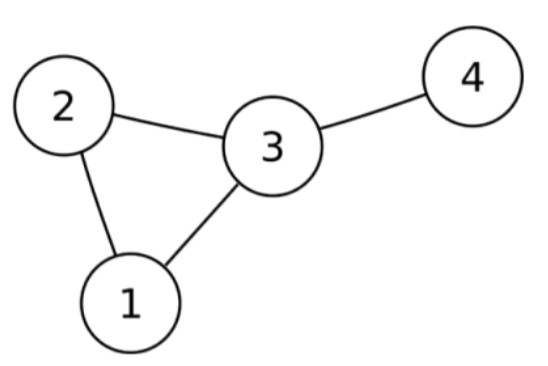
\includegraphics{Figures/grr}
\decoRule
\caption[A drawing of an undirected graph with 4 vertices and 4 edges.]{A drawing of an undirected graph with 4 vertices and 4 edges.}
\label{fig:la}
\end{figure}
Graph-based methods are considered a powerful tool for computer vision mainly in image processing and object matching. In early works, Graph based method was not used for modelling human actions, due to its complexity. But recently, this method has been proposed by many researchers. \\

Ta et al. [48] develop a graph matching algorithm on KTH and Weizmann datasets with state-of-the-art results. The objective of this approach is to calculate the similarity between two videos for instances of the graph model, rather than classifying the whole sequence to recognize the activity. The advantage of this method appeared in detecting multiple instances of activities occurring in the scene simultaneously without any reprocessing. \\

Brendel and Todorovic [49], proposed a method for modelling spatial temporal graphs of human activities. The ST-graphs model the ST-relationships between activity parts. In another word, the nodes corresponding of video segments, and the edges model the ST-relationships. This method enabled a fast training from segmented videos into more than 2000 space-time cube at multiple scale. The results were evaluated from UT interactions, Olympic sports and Weizmann datasets. \\

The disadvantage of graph-based representation is that the complexity of the graph dramatically increases when the number of nodes and edges grow. On the other hand, graphs cannot perform simple sums operations which make them useful for patterns classification and recognition.\\

To solve these problems, Graph embedding offer an alternative implementation, which allow basic operations to perform on graphs. Graph embedding convert graphs into a vector-based representation. It then become useful for conventional pattern recognition and complex statistical models. In [50], a novel graph-based method model human’s spatial features when performing a specific action. A discriminative approach is modelled where the graph is embedded as a feature vector on a synthetic data from KTH dataset, and an attributed graph is built in each frame to represent the human’s shape. Then the HMM is used to classify the actions.
\begin{figure}[ht]
\centering
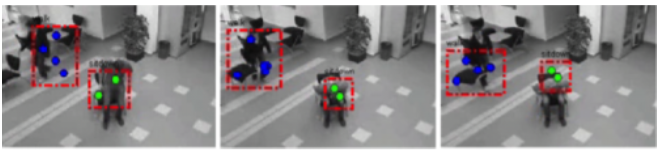
\includegraphics{Figures/gr1}
\decoRule
\caption[An example of using Graph method for HAR "37"]{An example of using Graph method for HAR[37].}
\label{fig:la}
\end{figure}\hfill \\

A related work on Embedding graph was developed using Spectral clustering technique in [37]. In this method, the author used the noisy track of an insect and construct the features using 3D object movements to discriminate between the action’s classes. Then perform the clustering algorithm K-mean to cluster the principle components of every odd eigenvectors of the affinity matrix.\\

Graphs are a flexible tool to represent the spatial temporal features of an activity or even between parts of the human body. That’s because Graphs are able to extract complex patterns and efficiently connecting them to each other. 
\subsection{Sequential Model}
\hspace{5mm} In sequential models, video sequences are considered to recognize human actions from a given set of sequential features. In this case recognition is performed by analyze the sequence corresponding to that activity in the video. Sequential are divided to two categories, Example based and state-based approach. Example based approaches use the training sample as a sequence of templates to describe human action classes. As a result, recognition is accomplished if the sequence of action is retrieved from the video sequence. However, State based approaches model the action as sequence of state with the corresponding associated probabilities. In this example, states refer to a particular spatial feature or small gestures which form an action. Then the recognition is achieved by calculating the probability that the sequence is generated in a video.

\subsubsection{Example Based Approaches}
\hspace{5mm} Example based method represent human activities as a template of the action’s execution. For an unlabeled video, the spatial vectors extracted from the video are compared to the template, if similarities in the observation were high between the features vector and the template, then the unlabeled video is classified as part of this action execution template. All the sequential method considers the variation of human actions, as every person perform actions differently.\\ 

Darel et al. [51] proposed a DTW (Dynamic time warping) for human gesture. DTW has been applied to temporal sequences of video, audio, and graphics data and it is a powerful algorithm for measuring two temporal sequences which might vary in speed. The author developed a real time system that recognize complex objects and human gestures by using a view-based representation which model the portion of the object used by the user in the recognized gestures. This was achieved by modelling the correlation scoring between the image frames and the template images as a function of time. Then the scores from the training videos are used to form the template. In this case, DTW was used to match the unseen video with the template which consider the variation in every action for each person.\\

Another example of using DTW was in [39] by Gavrilla and Davis. The authors aim to model the skeleton of the human body in each frame and tracking it by measuring its variation over time. This method used DTW algorithm to recognize human gestures like hand waving and hand clapping using the 3D body parts tracking.\\

Yacoob et al. used SVD method to decompose actions signals into a set of eigenvectors to form the action template or basis. This method recognizes actions by calculating the similarities between the input and the template from the coefficient of the activity template. A successful example for this method was recognizing “Walking” action.

\subsubsection{State Based Approaches}
\hspace{5mm} State based method model human’s activities as a sequence of activity states. A similarity measurement between the model and the input video sequence is generated from a sequence of feature vectors. This probability is modelled by two classification method, maximum likelihood estimation (MLE), maximum posterior probability (MAP). But recent works show that HMM and Dynamic networks (DBN) are widely used in state-based models.\\

Gao et al. [40] proposed a new method for HAR based on trajectory. They model activities using a discriminative latent variable from each action. Their model was based on Hidden conditional random fields (HCRF) as discriminative model, rather than generative. This method outperforms both HMM and CRF method on both real and synthetic data.
\begin{figure}[ht]
\centering
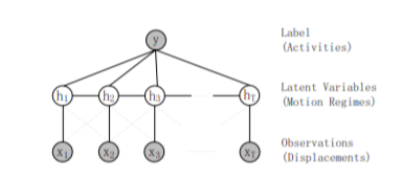
\includegraphics{Figures/HCRF}
\decoRule
\caption[A diagram of HCFR architecture for trajectory recognition "27".]{A diagram of HCFR architecture for trajectory recognition [27].}
\label{fig:la}
\end{figure}\\

Yamato et al. [28] present a method using HMMs. Their approach represents a single HMM for each activity which correspond to a particular sequence of feature vectors. HMM parameters are trained and used to recognize by measuring the similarity of the HMM and the input test video. This method, shows that HMM is applied to a set of time sequential images and transforming them into feature vector sequence, then these sequences are converted into symbols sequence by vector quantization. The system successfully recognized complex action such as playing tennis.\\

\begin{figure}[ht]
\centering
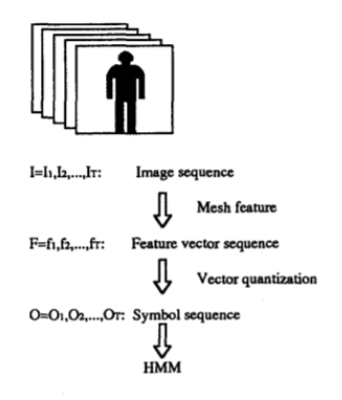
\includegraphics{Figures/qw}
\decoRule
\caption[Visualization of HMM architecture from applying Mesh feature on the image to use Vector quantization to convert the sequence into symbols "28".]{Visualization of HMM architecture from applying Mesh feature on the image to use Vector quantization to convert the sequence into symbols [28].}
\label{fig:la}
\end{figure}

An extension of the [28] was present by [29], using DBN to recognize two-person interactions. The recognition in this interaction is represented in terms of semantic verbal descriptions at different levels such as, individual body part at lower level and single person actions at middle level and two-person interactions at high level. DBN generate observations from multi hidden node at each frame. This experiment shows that the proposed model recognizes details interactions consisting of multiple body parts.\\

Sequential approaches are generally useful at modelling complex sequence consisting of smaller actions to more complex activities or gestures. State based approaches incorporate into other decision-making systems by calculating the probability of an action occurring. However, the disadvantage of state-based model is the algorithm generalization. To illustrate that, if an action occurs in the scene, and one state of this actions was missing due to partial occlusion, then it is difficult to recognize the actions. On the other hand, the other problem that face the sequential model, is the large number of data needed to model an effective system. 

\subsection{Syntactic Models}
\hspace{5mm} Syntactical model represents the activity as symbols where each symbol is a small atomic gesture. According to previous works in this domain, Context fee grammars (CFG), and Stochastic context-fee grammars (SCFG) have been used for HAR. Features are referred to the small atomic actions. In this section, methods are built upon lower level approaches to provide a higher-level activity representation.\\

In [30], Ivanov and Bobick modelled a HAR using SCFG approach. They divide the recognition to two section, where the lower level recognition is performed using probabilistic event detectors to proposed human detection at low level features. Then the output detectors give an input sequence for a stochastic context-fee grammar parsing mechanism. This method recognize activity of multiple, interacting objects.\\

Moore and Essa [31], extend on [30], by focusing on multi-task activities. Each action is labelled depending on visual and domain-specific information. They presented every action event as unique symbol, enabling a sequence of interactions to be described as an ordered symbolic string. The SCFG is developed to provide the structure of a semantical meaningful behavior over time. The method shows that parsing improves over 40\% and reduce the error to 87\%. It successfully collaborative tasks like cards games.\\

Syntactical methods are able to model a complicated activity from simple atomic gestures. However, this method is limited to number of gestures in an action, which make the model sensitive to any action’s variation over time. To illustrate that, if a sequence of a video doesn’t contain all the small gestures that can possibly happen, then the recognition is hard to perform. On the other hand, it is hard to form a model basis or production rule to cover all the possible events, as some videos contain an action that it is not part of the production rule. The main advantage of a Syntactical methods is their flexibility to be combined with simpler approach to model complex activities.

\subsection{Anomalies detection Models}
\hspace{5mm} A model for detecting anomalous behaviors is discussed in this section. In this model context are the main ingredient for such a system, as an anomaly may vary depending on the scene. The main difference in this model is that the majority of the models for HAR rely on offline learning and classification from set of labelled actions, but in anomalies HAR the abnormal activity is known, and the system must learn to differentiate this activity online. Another important difference is that abnormal activities appear with low probability with respect to the normal activity. \\

Anomalies detection in HAR is a well-researched area, and recently wide variety of methods were proposed. The performance of these method tends to be low due to factors such as scene clutter, occlusions and unsteady flow in the scene, and in complex scene like crowd anomalies detection, the low-level method to feature representation are unreliable. \\
Li et al. [52], proposed an approach that consider both appearance and dynamic using mixture dynamic texture models. Their method is implemented by model the discriminant saliency detector that produces spatial saliency scores, and a model of normal behavior from the training of the dataset that produce temporal saliency score. A dataset of densely crowded pedestrian walkways with non-staged, realistic anomalies is introduced and the model show state of the art results in anomalies detection. \\

Thida et al. [33], proposed a spatial temporal Laplacian Eigen map method to extract crowd activities from the scene. Using K-means the motion patterns were clustered in the embedded space and a multivariate Gaussian mixture model (GMM) is used to represent the motion features. The pairwise graph is built considering the visual context of spatial and temporal domain of the local patches. In this method the local probabilistic model learns not only to detect abnormal events in local and global contexts but to localize the abnormal region accurately.
\begin{figure}[ht]
\centering
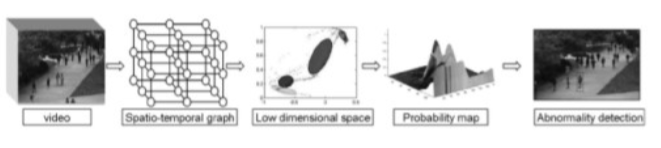
\includegraphics{Figures/add}
\decoRule
\caption[An illustration of the anomaly detection method for crowd activities "33".]{An illustration of the anomaly detection method for crowd activities [33].}
\label{fig:la}
\end{figure}
\newpage
Kratz and Nishino [34], present a novel statistical framework for modeling the spatial temporal motion in an extremely crowded environment by modeling the rich motion patterns in local areas of the scene. They used GMM in their method as a 3D distribution. The temporal relationship is captured by a distributed based HMM between local spatial temporal motion pattern, and the spatial relationship is captured by a coupled HMM. The proposed framework was able to detect unusual motion patterns in pedestrian activity such as normal traffic flow and traffic congestion.\\

\subsection{Research Questions}
\hspace{5mm} Based on literature review, several questions about the current research in HAR are raised to address the research gap. These questions will form the basis of this research. These questions include:\\
\begin{description}
    \item \textbf{Robust live detection system}\hfill \\
    Is this research study will succeed in addressing the challenges in improving live detection by reducing the computation cost and improving the accuracy?
   
    \item \textbf{Detecting human activity from sensors and visual data}\hfill \\
    Is the proposed method more scalable to adapt a model that run on time series sensor data, as well as video camera data? 

    \item \textbf{Normalization and Anomalies}\hfill \\
    Is adding an anomalies and applied data normalization will remove system confusion in recognizing action in a noisy environment?
    
    \item \textbf{Frequency domain using Statistical features}\hfill \\
    Is the proposed model in the thesis able to do trial and error to find the features for particular action?
    
    \item \textbf{Multi camera feature fusion} \hfill \\
    Will the network be flexible enough to be trained on multiple camera frame using a semantic technique that provide situational context?
    
    \item \textbf{Video frame segmentation}\hfill \\
    Are finding the mean and convariance projection matrix of the actor and the background the best approach to segment the video frame of the action execution?
    
\end{description}

\section{Research Methodology}
\subsection{Introduction}
\hspace{5mm} This chapter is organised as follows: The first part will focus on the software and the operation system used to program the algorithm and process the steps involved. Next, the popular human action dataset is introduced and used to as backbone for the thesis. Finally the proposed method is presented with a step by step explanation.
\subsection{Software Stack}
\hspace{5mm} The following section, give a brief explanation on the programming language and frameworks used that were used to extract frames from the videos data and build the neural networks.
\subsubsection{Operation System}
\hspace{5mm} The goal of choosing the technology stack to build such application, was to develop a piece of software that run on any OS version. Therefore, the method was implemented on UBUNTU 14.04 LTS (Trusty Tahr) for system reliability and code reproducibility. The code can also be scalable due to the stable working environment UBUNTU offer in its systems.
\begin{figure}[ht]
\centering

\includegraphics{Figures/u}
\decoRule
\caption[UBUNTU software logo "53".]{UBUNTU software logo [53].}
\label{fig:la}
\end{figure}

\subsubsection{Programming Language}
\hspace{5mm} The code is implemented in the interpreted high-level programming language Python. The reason for choosing this programming language is its features in dynamic type system and automatic memory management with support of multiple programming paradigms, such as object-oriented programming (OOP), imperative, functional and procedural and the support of large comprehensive standard library.
Python 3.6.2 version was used.

\begin{figure}[ht]
\centering

\includegraphics{Figures/python}
\decoRule
\caption[Python software logo "54"]{Python software logo [54].}
\label{fig:la}
\end{figure}

\subsubsection{Anaconda Distribution}
\hspace{5mm} Anaconda is an optimized graphical user interface (GUI) that allow the user to launch applications and manage working environment without using command-line commands. It also helps in searching for packages using their cloud data or the local anaconda repository. Anaconda 4.4.0 bit 64 is used to manage all the packages versions and deployments. In another case, Anaconda is used to run pre-built scripts, by simply initializing the working directory and typing the script name, which eliminate using any IDE.
\begin{figure}[ht]
\centering

\includegraphics{Figures/anaconda}
\decoRule
\caption[Python software distribution Anaconda "55".]{Python software distribution Anaconda [55].}
\label{fig:la}
\end{figure}
\subsubsection{Jupyter Lab}
\hspace{5mm} Jupyter lab is an extension of the project Jupyter notebook that offer an extensible environment for reproducible and interactive computing. The project takes advantage of using Jupyter lab notebook, terminal, text editor and file browser, offering an end-to-end tool with its own eco-system.\\

For documentation purposes and implementation, Jupyter Lab was used as the main GUI for providing rich comment on the code and updating the cell for optimization and debugging. Jupyter Lab is also used to train the model and visualize the neural network architecture.
\begin{figure}[ht]
\centering

\includegraphics{Figures/jupyter_lab}
\decoRule
\caption[Jupyter Lab software logo "56".]{Jupyter Lab software logo [56].}
\label{fig:la}
\end{figure}

Figure 3.5 shows Jupyter lab interface.\\
\begin{figure}[ht]
\centering
\includegraphics{Figures/jl1}
\decoRule
\caption[Jupyter lab interface and its functionality.]{Jupyter lab interface and its functionality.}
\label{fig:la}
\end{figure}

\section{KTH Dataset}
\hspace{5mm} An overview of the dataset used is presented in following section.\\

The KTH action datasets have been introduced by Shnuld et al. [54]. The video database contains 6 types of human actions. Actions are: Walking, Running, Jogging, Jumping, Hand waving and Hand clapping. They are performed several times by 25 subjects. Each subject performs actions in four different scenarios. Scenarios are outdoors (s1), outdoors with scale variation (s2), outdoors with different clothes (s3) and indoors (s4). All recorded videos are taken over homogeneous background and are down-sampled to 120x160 spatial resolution by the authors. The sequences are recorded using a static camera with 25 frames per second (fps) rate, and have a length of four second for each in average. According to authors, sequences are divided with respect to the subjects into training set of 8 persons, a validation set of 8 persons and a test set of 9 persons. All videos sequences are stored using AVI video file format. Overall, there are 600 videos for combination of 25 subjects, 6 actions and 4 scenarios. 
\begin{figure}[ht]
\centering
\includegraphics{Figures/dt1}
\decoRule
\caption[visualization of KTH dataset. Columns represent different types of human actions, rows represent different scenarios, for each of the 6 actions categories "54"]{visualization of KTH dataset. Columns represent different types of human actions, rows represent different scenarios, for each of the 6 actions categories [54].}
\label{fig:la}
\end{figure}
KTH dataset present major challenges, like low resolution, scale changes, illumination variations, shadows, different people, different scenarios, cloth variations, inter and intra action speed variations. The author proposed an evaluation method by splitting-based evaluation scheme and have one person out cross validation evaluation scheme.\\

The spatial dimensions of the video are 160x120 (width x height). Using Numpy (Python library) loading a single video from the entire dataset will have the shape of the array:(1,515,120,160,3).\\
This representation indicates that:
\begin{itemize}
\item There is 1 video.
\item The video has 515 frames.
\item The video spatial dimension is 120x160 pixels.
\item There are 3 channels for each frame - Red (R), Green (G) and Blue (B).
\end{itemize}
To read the entire dataset, the same methodology will be followed.\\

\begin{figure}[ht]
\centering
\includegraphics{Figures/wa1}
\decoRule
\caption[Matrix visualization of the action walking from KTH dataset.]{Matrix visualization of the action walking from KTH dataset.}
\label{fig:la}
\end{figure}\\

From the above visualization, each activity involves the movement of the whole body. Some of the frames might be empty like in the image below, due to action variations over time which make some of the frames redundant and empty.

\subsection{Implementation}
\hspace{5mm} In this section we present a method to recognize human actions from an input video sequence. The aim of this method is to create a model that can detect basic human actions. The model is given a set of videos, where each video consists of an action performed by a human. The label of a video is the action being performed. The model is then training to differentiate between various human actions and understand this relationship, and then it should predict the label of an unseen video. The following gives an overall explanation of the method used to build a supervised classification model. Building a ML model consist of multiple parts:
\begin{itemize}
\item Clean Data.
\item Execute the defined networks.
\item Reshaped to fit into the model. 
\item Make prediction.
\end{itemize}

The following diagram illustrate the steps for building this ML model.\\
\begin{figure}[ht]
\centering
\includegraphics{Figures/m}
\decoRule
\caption[Visualization of the machine learning model used for this task.]{Visualization of the machine learning model used for this task.}
\label{fig:la}
\end{figure}
\newpage
As shown in figure 3.8, the implementation is consisting of different important steps. Each step has to satisfy the input of the next one in order to achieve the final results. It starts with importing all the dependencies and libraries. They are pre-built framework for complex mathematical calculation which is needed to perform the calculation correctly.\\

\begin{figure}[]
\centering
\includegraphics{Figures/fn}
\decoRule
\caption[Flowchart of building the neural networks from start to end.]{Flowchart of building the neural networks from start to end.}
\label{fig:la}
\end{figure}
\newpage
The following steps is splitting the data to three main sections, training, validation and test set:
\begin{figure}[ht]
\centering
\includegraphics{Figures/ds}
\decoRule
\caption[Python command lines responsible of splitting the data to train, validation and test.]{Python command lines responsible of splitting the data to train, validation and test.}
\label{fig:la}
\end{figure}
First the data is divided to training and test set respectively to 66.67\% and 33.33\%. Then taking approximately 25\% of the training data for validation. At the end 598 videos are then divided to 300 videos for training set, 98 videos for validation set and 200 videos for the test set as shown below. 
\begin{figure}[ht]
\centering
\includegraphics{Figures/datasplitoutput}
\decoRule
\caption[Splitting the data to three sets]{Splitting the data to three sets.}
\label{fig:la}
\end{figure}
\newpage

\subsubsection{Data Preprocessing}
\begin{figure}[ht]
\centering
\includegraphics{Figures/dp}
\decoRule
\caption[A step-by-step flowchart for data preprocessing.]{A step-by-step flowchart for data preprocessing.}
\label{fig:la}
\end{figure}
The essential step in every model, is data pre-processing. This was implemented in utils.pyfile. In this file there is a Python script that read in the video frame by frames. These videos were recorded at a frame rate of 25fps. In general, within a second the human does not perform a recognizable movement. This implies that most of the frames in the videos are redundant. Only a section of all the frames in a video are needed to extract. Following this procedure, the input data will help to model train faster and avoid over-fitting issues.\\

In utils.py, different method was used to extract frames. The following are the strategies used:
\begin{itemize}
\item Extracting a fixed number of frames from the overall frames in the video. For example, the first 250 frames, or the first 10 seconds of the video.
\item Extracting a fixed number of frames each second from the video. For example, extracting 10 frames per second from a video of 5 seconds. This will return a total of 50 frames from the whole video.
\end{itemize}
\hspace{5mm} The latter one, is used in extracting the frames from the video datasets, as this approach extract the frames sparsely and uniformly from the entire datasets.
Each frame will have to be reshaped and resized to the required size. Hence each frame needs to have the same spatial dimension such as height and weight. On the other hand, to reduce the model complexity and guarantee better performance and recognition, the frames are converted to grayscale.\\

One of the important parts in data preprocessing is Normalization, where the standard pixel value is from 0 to 255. For a grayscale images, the value of the pixel is a single number that represent the brightness rate of the pixel. The most common used pixel format is byte image, where the pixel number is stored as an 8-bit integer giving an image the standard 0 to 255 values. Typically, zero is taken to be very black, and 255 taken to be very white. However, these values are too complicated for the model, and normalizing them will help the model the converge faster and have better performance. To achieve such a performance, different normalization approach can be applied, such as:
\begin{itemize}
\item \textbf{Z-score Normalization}- Which determine the Standard deviation value from the mean value of the data.
\item \textbf{Min-Max Normalization}- Which make the value of the pixel to be from 0 to 1, instead of 0 to 255.
\end{itemize}
\hspace{5mm} The implementation of utils,py will produce a 5-dimensional tensor shape of:
(<number  of videos>,<number of frames>,<width>,<height>,<channels>)
Where channels can have 1 for grayscale format and 3 for an RGB format, and the number of frames are the same for the whole dataset videos.
To convert the categorical variables into a form that could be provided to the proposed ML algorithm, a one hot encoding is used. One hot encoding will help the algorithms to do a better prediction on the data and will convert the categorical data to numerical data which consist of two steps:
\begin{itemize}
\item \textbf{Integer Encoding}- It is the first step of the converting methodology, where each unique category is assigned to an integer value. To illustrate that based on the data used, “walking” is 1, “running” is 2, and “jumping” is 3. This is a label encoding or integer encoding technique which work in reverse way. The integer value has a natural ordered relationship between each other, and ML algorithms have the ability to understand and harness the relationship between them.  For some variables, this technique might be enough.
\item \textbf{One-Hot Encoding}- In some case, categorical variables without any relationship exists, the integer encoding is not enough, and sometimes not scalable on dataset with large categories. To make the model assume a natural ordering between categories may have a bad impact on the data, and May results in poor performance and unexpected results. For example, predicting half of the categories and fail in build a relationship between the other categories. For KTH datasets, a one-hot encoding is applied to the integer representation. The integer encoded variable is removed and a new binary variable is added for each unique integer value. The method is also called Binarization. In the given data sets, there are 6 categories and therefore 6 binary variables are applied. A 1 value is placed in the binary variable for a specific actions label and 0 values is placed the other actions.
\end{itemize}

Tables 3.1 and 3.2 show the differences between a one-hot encoded datasets labels and non-one-hot encoding one.
\hspace{5mm} 
\begin{table}[]
\centering
\begin{tabular}{|c|c|}
\hline
\textbf{Class Label} & \textbf{Mapped Integers} \\ \hline
Boxing               & 0                        \\ \hline
Handclapping         & 1                        \\ \hline
Handwaving           & 2                        \\ \hline
Walking              & 3                        \\ \hline
Jogging              & 4                        \\ \hline
Running              & 5                        \\ \hline
\end{tabular}
\caption{How the class labels are mapped before one-hot encoding}
\label{my-label}
\end{table}

\begin{table}[]
\centering
\begin{tabular}{|c|c|c|c|c|c|c|}
\hline
\textbf{Class Label} & \textbf{0} & \textbf{1} & \textbf{2} & \textbf{3} & \textbf{4} & \textbf{5} \\ \hline
Boxing               & 1          & 0          & 0          & 0          & 0          & 0          \\ \hline
Handclapping         & 0          & 1          & 0          & 0          & 0          & 0          \\ \hline
Handwaving           & 0          & 0          & 1          & 0          & 0          & 0          \\ \hline
Walking              & 0          & 0          & 0          & 1          & 0          & 0          \\ \hline
Jogging              & 0          & 0          & 0          & 0          & 1          & 0          \\ \hline
Running              & 0          & 0          & 0          & 0          & 0          & 1          \\ \hline
\end{tabular}
\caption{How the class labels are mapped after one-hot encoding.}
\label{my-label}
\end{table}

\subsubsection{Model Hyper-parameters}
\hspace{5mm} Model variables are an essential part and the basis of building a ML model. Even tough, with the existing of all the computational power, choosing the right variables is by far one of the hardest problems occur when building a model, and finding them is done by fine tuning the model. The following sections give a comprehensive explanation about model hyper-parameters.\\

Hyperparameters express higher-level properties of the model such as its complexity and how fast it should learn. They cannot be directly learned from the regular training process and cannot be estimated from data. Usually Hyper-parameters are initialized and fixed before the actual training process begin.\\

Overall, Hyperparameters:
\begin{itemize}
\item Are considered higher level concepts about the model.
\item Need to be predefined as they cannot be learned from the data.
\item Can be decided by setting different values, choosing the values that test better and training models.
\end{itemize}\\

Some of the hyper-parameters example are:
\begin{itemize}
\item Learning rate – is the size of the gradient descent step and how much to update the weight in the optimization algorithm. To name few methods used to initialize the learning rate such as:
\begin{itemize}
\item Fixed learning rate.
\item Gradually learning rate.
\item Momentum based learning rate.
\item Adaptive learning rates.  
\end{itemize}
\item \textbf{Number of epochs} – Is the number of times the whole dataset has to go through the NN. The number of epochs depend on the gap between the test error and the training error.
\item \textbf{Batch size} – In convolutional networks mini-batch are usually preferable, rather than batch. The best values for mini-batch are between 16 and 128.
\item \textbf{Activation function} – Is used to introduce non-linearity to the network. For convolutional networks, RELU function is usually used, but for alternative Sigmoid, Tanh activation functions can be used depending on the task. 
\item \textbf{Number of hidden layers} – They play an important role in improving the test error results, and choosing them should be wisely. Having a small number of units may lead to underfitting, while having more units might be manageable with some regularization methods.
\item \textbf{Weight initialization} – It recommended to initialize the weight with small random number to avoid “dead neuron”. However, a small weight value can lead to vanishing gradient or zero gradient. A uniform distribution weight works well in a NN model.
\item \textbf{Dropout for regularization} – It is a regularization method used to avoid overfitting figures in the NN. Dropout drops neurons from each hidden layer according the desired probability for simplicity.
\item \textbf{Grid search} – It is a method to perform a hyperparameters optimization. It then searches all parameter combinations for given values.
\item \textbf{Randomized search} – It samples a predefined number of candidates from a parameter space with a specified distribution.  
\end{itemize}
\hspace{5mm} In this Thesis, multiple models will be built tested and compared. For that reason, hyperparameters are in the process of fine tuning, and they differ for every model.


\subsubsection{Model Parameters}
\hspace{5mm} Model parameters are the properties of the training data which the model would be learned by ML model such as weight and biases. However, in this implementation variety of parameters were configured for both convolutional layers and pooling layers.\\

For Convolutional layers:
\begin{itemize}
\item \textbf{Filters}- The number of feature maps needed for the convolutional layer output.
\item \textbf{Kernel size} - This is the size of the filter that will convolve on all the axes of the input data to form a feature map.
\item \textbf{Strides} - The number of pixels needed to shift the convolutional window.
\item \textbf{Padding} - It either “Valid” when the input gets cropped, or “Same” when the input is padded with zeros to main a similar dimension.
\item \textbf{Activation }- As mentioned in the previous section, there are many activation functions to be used, however, RELU is proven to work best with DNN, due to its non-linearity, and its ability to eliminate the vanishing gradient problem).
\end{itemize}\\

For pooling layers:
\begin{itemize}
\item \textbf{Pool size} - window size (height and width).
\item \textbf{Strides} - The number of pixels needed to shift the convolutional window.
\item \textbf{Padding} - It either “Valid” when the input gets cropped, or “Same” when the input is padded with zeros to main a similar dimension.
\end{itemize}

\subsubsection{Sequential CNN model}
\hspace{5mm} In this section, the layers construction of the NN model is covered. The model is using a combination of parameters and hyperparameters mentioned above. To build the model the utils.py script is used to extract the frame from each video sequence. The following section explain the model architecture.\\

Keras API was chosen to build the neural network stack based on the sequential model. The sequential model is a linear stack of layers that form the statistical model. Creating a sequential model is possible by passing a list of layers instances to the constructor via  model.add() method like below:
\begin{figure}[ht]
\centering
\includegraphics{Figures/se1}
\decoRule
\caption[How to import the sequential library from Keras API. The code used to build the sequential model.]{How to import the sequential library from Keras API. The code used to build the sequential model.}
\label{fig:la}
\end{figure}
The first layer in a sequential model is receiving information about its input shape, because the model needs to know what input shape it should expect. This can be implemented by passing an input\_shape argument to the first layer. \\

Numpy is a popular Python package for scientific computation was used for storage and processing the videos. Numpy offer a much faster processing than the in-built python lists with lots of extra functionalities. For that reason, Keras models are usually trained on NumPy arrays.

\begin{figure}[ht]
\centering
\includegraphics{Figures/suma1}
\decoRule
\caption[The code written in python, showing the neural networks layers.]{The code written in python, showing the neural networks layers.}
\label{fig:la}
\end{figure}
In this model a stack of 9 layers neural networks is built. The following is the network specification in each layer:

\begin{itemize}
    \item \textbf{Con3D layer} is spatial convolutional over volume. This layer produces a convolutional kernel which convolve with the input layer to create an output tensor. This layer takes argument as following:\\
    \noindent\fcolorbox{black}{white}{%
\minipage[c]{\dimexpr1.0\linewidth}
   \textcolor{dkgreen}{// Con3D Layer } \\
   \textcolor{blue}{keras.layers.Conv3D}(\textcolor{red}{filters},\textcolor{red}{kernel\_size},\textcolor{red}{strides}=(1,1,1),\textcolor{red}{padding}=valid,\\
   \textcolor{red}{data\_format}=None,\textcolor{red}{dilation\_rate}=(1,1,1),\textcolor{red}{activation}=None,\\
   \textcolor{red}{use\_bias}=True,\textcolor{red}{kernel\_initializer}='glorot\_uniform',\\
   \textcolor{red}{bias\_initializer}='zeros',\textcolor{red}{kernel\_regularizer}=None,\\
   \textcolor{red}{bias\_regularizer}=None,\textcolor{red}{activity\_regularizer}=None,\\
   \textcolor{red}{kernel\_constraint}=None,\\
   \textcolor{red}{bias\_constraint}=None)
\endminipage}
    \begin{itemize}
        \item \textbf{Filters:} The number of output filters in the convolutional. It is an integer of the dimensionality of the output space. 
        \item \textbf{Kernel size:} A list of 3 argument specifying the depth, width and height of the 3D convolutional window. A single integer will specify the same spatial dimensions of the filter.
        \item \textbf{Strides:} A list of 3 argument specifying the strides of the convolutional along each spatial dimension. A single integer will specify the same spatial dimensions of the filter.
        \item \textbf{Padding:} It can be either “same” or “valid” and both are case sensitive.
        \item \textbf{Data format} A string of either “channel\_last” or “channel\_first” which specify the ordering of the dimension in the inputs. 
        \item \textbf{Dilation rate:} A list of 3 integers specifying the dilation rate for convolutional. A single integer will specify the same spatial dimensions of the filter.
        \item \textbf{Activation:} A mathematical function for the classifier it can be “RELU”, “Tanh”, “Leaky RELU”, “Sigmoid”, etc.
        \item \textbf{Use bias:} It is a Boolean operation of whether the layer uses a bias vector.
        \item \textbf{Kernel initializer:} It initializes the kernel weight matrix.
        \item \textbf{Kernel regularizer:} A regularizer function applied to the kernel weight matrix.
        \item \textbf{Activity regularizer:} A regularizer function applied to the bias vector.
        \item \textbf{Kernel constraint:} A constraint function applied to the kernel matrix.
        \item \textbf{Bias constraint:} A constraint function applied to the kernel matrix.
    \end{itemize}
    \newpage
    In this model the first Con3D layer is set according to these specifications:
    \begin{figure}[ht]
    \centering
    \includegraphics{Figures/c31}
    \decoRule
    \caption[A piece of the code written to build the Conv3D layer.]{A piece of the code written to build the Conv3D layer.}
    \label{fig:la}
    \end{figure}\hfill \\
    Note that if any of the previous specification are not specified in the layer, they will be considered None by default.
    The following figure 3.18 is a mathematical demonstration on how the convolutional operation perform on an image. 
    \begin{figure}[ht]
    \centering
    \includegraphics{Figures/matrix1}
    \decoRule
    \caption[A piece of the code written to build the Conv3D layer.]{A piece of the code written to build the Conv3D layer.}
    \label{fig:la}
    \end{figure}\hfill \\
    The matrix is then shifted by one row and one column at a time. After multiplying both of the matrices above, the result is a new 4x4 matrix with new pixel distribution. Below is an example of the calculation of one of the pixel cells.\hfill \\
    \item \textbf{Max Pooling3D layer:} It is function to reduce the spatial size of the representation using the max operation to reduce the quantity of parameters and the computation time in the network in order to control overfitting.\\
    Max Pooling 3D layer takes argument as following:\\
    \noindent\fcolorbox{black}{white}{%
    \minipage[c]{\dimexpr1.0\linewidth}
   \textcolor{dkgreen}{// Max Pooling 3D Layer }\hfill \\
   \textcolor{blue}{keras.layers.MaxPooling3D}(\textcolor{red}{pool\_size}=(2,2,2),\textcolor{red}{strides}=None,\\
   \textcolor{red}{padding}='valid',\textcolor{red}{data\_format}=None)
\endminipage}
\begin{itemize}
    \item \textbf{Pool size:} A list of 3 arguments that will have the dimension size of the 3D input in each dimension.
    \item \textbf{Strides:} A list of 3 arguments of strides values, it also can be none.
    \item \textbf{Padding:} It can be either “same” or “valid”.
    \item \textbf{Data format:} A string of either “channel\_last” or “channel\_first” which specify the ordering of the dimension in the inputs.\hfill \\
    It does have an input data shape if:
    \begin{itemize}
        \item \textbf{data\_format}= ‘channel\_last’, a 5D tensor with the following shape will be generated: (batch\_size, pooled\_dim1, pooled\_dim2, pooled\_dim3, channels).
        \item \textbf{Data\_format}= ‘channel\_first’, a 5D tensor with the following shape will be generated: (batch\_size, channels, pooled\_dim1, pooled\_dim2, pooled\_dim3).\hfill \\
        \end{itemize}
    In this model the first MaxPooling3D layer is set according these specifications:\hfill \\
    \begin{figure}[ht]
    \centering
    \includegraphics{Figures/mp1}
    \decoRule
    \caption[A piece of the code written to build the MaxPooling layer.]{A piece of the code written to build the MaxPooling layer.}
    \label{fig:la}
    \end{figure}\hfill \\
    Figure 3.20 is a mathematical demonstration of how the max pooling 3D operation perform on an image with a pooling filter of size 2x2 and stride of 2.\hfill \\
    \newpage
    \begin{figure}[ht]
    \centering
    \includegraphics{Figures/mp}
    \decoRule
    \caption[A visualization of max pooling layer.]{A visualization of max pooling layer.}
    \label{fig:la}
    \end{figure}
\end{itemize}\hfill \\
\item \textbf{Global average pooling 3D:} it was proposed in [38] as a replacement of the traditional fully connected layer in CNN. it does have same functionality as the max pooling 3D layer. However, the global average pooling (GAP) are more extreme type of dimensionality reduction, where a tensor of h x w x d is reduced in size to have a dimension of 1 x 1 x d. It reduces each of the dimension h x w feature map to a single number by taking the average of all hw values.\hfill \\
GAP 3D layer takes argument as following:\hfill \\
\noindent\fcolorbox{black}{white}{%
    \minipage[c]{\dimexpr1.0\linewidth}
   \textcolor{dkgreen}{// GAP 3D Layer  }\hfill \\
   \textcolor{blue}{keras.layers.GlobalAveragePooling3D}(\textcolor{red}{data\_format}=None)
\endminipage}
\begin{itemize}
    \item \textbf{Data format:} It contains a single string which can be either “channels\_last” or “channels\_first”.  In this case, it is not specified with any argument, that’s mean that it will be “channels\_last by default”.\hfill \\
\end{itemize}
\newpage
Figure 3.21 is a mathematical demonstration on how the global average pooling operation perform on an image with dimension of 6x6x3.\\
 \begin{figure}[ht]
    \centering
    \includegraphics{Figures/gap1}
    \decoRule
    \caption[A visualization of the GAP layer reducing the dimension of an image with 6x6x3 image to 1x1x3 "55"]{A visualization of the GAP layer reducing the dimension of an image with 6x6x3 image to 1x1x3 [55].}
    \label{fig:la}
    \end{figure}\hfill \\
In this model the GAP layer is set according these specifications:\\
 \begin{figure}[ht]
    \centering
    \includegraphics{Figures/GAPcode}
    \decoRule
    \caption[A piece of the code written for GAP layer.]{A piece of the code written for GAP layer.}
    \label{fig:la}
    \end{figure}
    \item \textbf{Dense layer or fully connected layer}: It is always the layer that comes after several convolutional and max pooling layers. The neurons in the dense layer have connections to all activations in the previous layer. These activations are regularly computed with a matrix multiplication prior to a bias offset.
    \newpage
    Dense layer takes argument as following:\hfill \\
    \noindent\fcolorbox{black}{white}{%
    \minipage[c]{\dimexpr1.0\linewidth}
   \textcolor{dkgreen}{// Dense Layer  }\hfill \\
   \textcolor{blue}{keras.layers.Dense}(\textcolor{red}{units},\textcolor{red}{activation}=None,\textcolor{red}{use\_bias}=True,\\
   \textcolor{red}{kernel\_initializer}='glorot\_uniform',\textcolor{red}{bias\_initialize}='zeros',\\
   \textcolor{red}{kernel\_regularizer}=None,\textcolor{red}{bias\_regularizer}=None,\\
   \textcolor{red}{activity\_regularizer}=None,\textcolor{red}{kernel\_constraint}=None,\\
   \textcolor{red}{bias\_constraint}=None)
\endminipage}
\begin{itemize}
    \item \textbf{Units:} It is positive integer of the outer space dimensionality.
    \item \textbf{Activation:} A mathematical function for the classifier it can be “RELU”, “Tanh”, “Leaky RELU”, “Sigmoid”, etc.
    \item \textbf{Use bias:} It is a Boolean operation of whether the layer uses a bias vector.
    \item \textbf{Kernel initializer:} It initializes the kernel weight matrix.
    \item \textbf{Bias initializer:} It initializes the bias vector.
    \item \textbf{Kernel regularizer:} A regularizer function applied to the kernel weight matrix.
    \item \textbf{Bias regularizer:} A regularizer function applied to the bias vector.
    \item \textbf{Activity regularizer:} A regularizer function applied to the layer.
    \item \textbf{Kernel constraint:} It is the constraint function applied to the weight matrix of the kernel.
    \item \textbf{Bias constraint:} It is the constraint function applied to the weight matrix of the bias vector.\hfill \\
    In this model the dense layer is set according these specifications:\hfill \\
    \begin{figure}[ht]
    \centering
    \includegraphics{Figures/dl}
    \decoRule
    \caption[A piece of the code written to build the dense layer.]{A piece of the code written to build the dense layer.}
    \label{fig:la}
    \end{figure}\hfill \\
    Above is showing a dense layer is applied to the hidden layer with RELU activation function, and another dense layer for the output layer using SoftMax activation function, which always used for predicting the label of the video.\\
    Finally, after building the model layers and connecting all the layer with each other, a layer summary is being executed to show the output shape of each layer and their corresponding parameters. This was performed using model.summary(). At the end, the model is consisting of 793,558 total parameters.
    \newpage
    \begin{figure}[ht]
    \centering
    \includegraphics{Figures/s}
    \decoRule
    \caption[The model summary.]{The model summary.}
    \label{fig:la}
    \end{figure}\hfill \\
    The below diagram, shows the stack of layers of the proposed CNN model:
    \begin{figure}[ht]
    \centering
    \includegraphics{Figures/cnnmm}
    \decoRule
    \caption[Sequential model architecture.]{Sequential model architecture.}
    \label{fig:la}
    \end{figure}\hfill \\
In term of compiling the model, before the training start the learning process should be configured. This is done by model.compile(). It usually receives three arguments:
\end{itemize}
 \begin{figure}[ht]
    \centering
    \includegraphics{Figures/compill}
    \decoRule
    \caption[The command line responsible of compiling the model.]{The command line responsible of compiling the model.}
    \label{fig:la}
    \end{figure}\hfill \\
    \begin{enumerate}
        \item \textbf{Loss function:} The model will try to minimize it. It is usually the string identifier of an existing loss function such as “mean\_squared\_error”, “mse”, “binary\_crossentropy”, etc. However, in this case “categorical\_crossentropy” is used because the networks is dealing with multi-class classification problem.
        \item \textbf{Optimizer:} It can be the string identifier of an existing optimizer such as “rmsprop”, “adagrad, “nadam”, etc. In this case, “adam” optimizer is used as it has the following criteria:
        \begin{itemize}
            \item learning rate (lr): float $>$ 0.
            \item beta\_1 a float number between 0 and 1, but generally closer to 1.
            \item beta\_2 a float number between 0 and 1, but generally closer to 1.
            \item Epsilon a float number greater than 0, float $>$ 0, as a fuzz factor.
            \item Decay as a float number greater than 0, float $>$ 0. It is added to the learning rate over each update.
            \item Amsgrad as Boolean function.\\
            The specifications of Adam optimizer algorithm were taken from the paper [37].
        \end{itemize}
        \item \textbf{List of metrics:} It is set to “accuracy” for any classification problem. It is also the string of an existing metric function.\\
        This receive set of arguments as below:
    \end{enumerate}
    This receive set of arguments as below:\\
    \noindent\fcolorbox{black}{white}{%
    \minipage[c]{\dimexpr1.0\linewidth}
   \textcolor{dkgreen}{// Model Checkpoint  }\hfill \\
   \textcolor{blue}{keras.callbacks.ModelCheckpoint}(\textcolor{red}{monitor}='val\_loss',\textcolor{red}{verbose}=0,\\
   \textcolor{red}{save\_best\_only}=False,\textcolor{red}{save\_weights\_only}=False,\textcolor{red}{mode}='auto',\\
   \textcolor{red}{period}=1)
\endminipage}
 In this model the Model.fit() function has been created as below:
\begin{itemize}
    \item \textbf{File path:} It is the path name to where the file will be saved.
    \item \textbf{Monitor:} The quantity to be monitored.
    \item \textbf{Verbose:} it can mode 0 or mode 1.
    \item \textbf{Save best only:} If it is True, then the latest model will not be overwritten the previous one.
    \item \textbf{Mode:} takes one of these arguments “auto”, “min”, “max”.
    \item \textbf{Save weight only:} this will make the best model to be saved.
    \item \textbf{Period:} It is the number of epochs between checkpoints.
\end{itemize}
In this model the ModelCheckPoint() function has been created as below:
\begin{figure}[ht]
    \centering
    \includegraphics{Figures/ef1}
    \decoRule
    \caption [A piece of code written for "ModelCheckPoint" function.]{A piece of code written for "ModelCheckPoint" function.}
    \label{fig:la}
    \end{figure}\hfill \\
    Not all arguments are used. Unused arguments are set to None by default.\\

At this stage the model is fully loaded and ready to be trained. model.fit() is used to run the model and start training. 
model.fit() command line takes arguments as follows:\\
\noindent\fcolorbox{black}{white}{%
    \minipage[c]{\dimexpr1.0\linewidth}
   \textcolor{dkgreen}{// Fit model  }\hfill \\
   \textcolor{blue}{fit}(\textcolor{red}{x}=None,\textcolor{red}{y}=None,\textcolor{red}{batch\_size}=None,\textcolor{red}{epochs}=1,\textcolor{red}{verbose}=1,\textcolor{red}{callbacks}=None,\\
   \textcolor{red}{validation\_split}=0.0,validation\_data=None,\textcolor{red}{shuffle}=True,\textcolor{red}{class\_weight}=None,\\
   \textcolor{red}{sample\_weight}=None,\textcolor{red}{initial\_epoch}=0,\textcolor{red}{steps\_per\_epoch}=None,\\
   \textcolor{red}{validation\_steps}=None)
\endminipage}
\end{itemize}
\begin{itemize}
    \item \textbf{X:} A list of NumPy arrays for the training data, because the model has multiple inputs.
    \item \textbf{Y:} A list of NumPy arrays for the target data, because the model has multiple outputs.
    \item \textbf{Batch size:} It is the number of samples in each gradient update.
    \item \textbf{Epochs:} It is the iteration performed across the X and Y dataset.
    \item \textbf{Verbose:} It is verbosity mode, which can be 0, 1 or 2.
    \item \textbf{Callbacks:} Applying the call back function during training.
    \item \textbf{Validation split:} It is float between 0 and 1.
    \item \textbf{Validation data:} Evaluating the loss and other metrics after each epoch.
    \item \textbf{Shuffle:} It can a Boolean function or a string.
    \item \textbf{Class weight:} It is used for weighting the loss function.
    \item \textbf{Initial epoch:} It can be either integer or None. It is number of steps before one epoch.
    \item \textbf{Validation steps:} It is the total number of steps to validate before stopping.
\end{itemize}
 In this model the Model.fit() function has been created as follows:
 \begin{figure}[ht]
    \centering
    \includegraphics{Figures/fit1}
    \decoRule
    \caption [A piece of code written for "Model.fit()" function.]{A piece of code written for "Model.fit()" function.}
    \label{fig:la}
    \end{figure}\hfill \\
 All the other no specified parameters will be None by default.
 Over the 40 epochs, the model receives different values for the weight. However, the highest value must be saved for future uses. The weight is (.h5) format. Saving the weight is an essential part of building a ML model, as it helps saving the model architecture and load the layers with the same name.
model.load\_weights() takes only one argument which is the name of the model architecture previously saved. 
\begin{figure}[ht]
    \centering
    \includegraphics{Figures/loadweight}
    \decoRule
    \caption [A piece of the written code to load the model weight.]{A piece of the written code to load the model weight.}
    \label{fig:la}
    \end{figure}\hfill \\
 After saving the best weight and loading it to evaluate the model accuracy of the unseen data. The test set has been kept for evaluation. 
In this implementation model.evaluate() is used to predict the model accuracy. During the evaluation the model will return the loss value and metrics values for the model in the test mode, and the computation are usually done in batches to speed to process.
model.evaluate() command line takes arguments as follow:
\begin{figure}[ht]
    \centering
    \includegraphics{Figures/ev}
    \decoRule
    \caption [A piece of the written code to perform the evaluation step.]{A piece of the written code to perform the evaluation step.}
    \label{fig:la}
    \end{figure}\hfill \\
    
Usually model.evaluate() take several arguments to perform this step. The common arguments are below:\\
 \noindent\fcolorbox{black}{white}{%
    \minipage[c]{\dimexpr1.0\linewidth}
   \textcolor{dkgreen}{// Evaluate the model}\hfill \\
   \textcolor{blue}{evaluate}(\textcolor{red}{x}=None,\textcolor{red}{y}=None,\textcolor{red}{batch\_size}=None,\textcolor{red}{verbose}=1,\textcolor{red}{sample\_weight}=None,\\
   +
   \textcolor{red}{steps}=None)
\endminipage}
 \begin{itemize}
     \item \textbf{X:} It is the NumPy array of the input data if it is a multi-class model.
     \item \textbf{Y:} It is the NumPy array of the target data if the model is multi-class.
     \item \textbf{Batch size:} It is the number of samples per evaluation step. The default value is 32, but in this model, it is initialized to 16.
     \item \textbf{Verbose:} It is the verbosity mode. 0 for silent and 1 for progress bar.
     \item \textbf{Sample weight:} It is an optional NumPy array of weighs for the test data.
     \item \textbf{Steps:} It either integer or None. 
     
 \end{itemize}
\subsection{Summary}
\hspace{5mm} In this chapter, a step by step explanation of proposed is given. First, we introduce our software tools and the popular dataset used for the thesis. Then, we discuss and explain the convolutional neural networks model was proposed to model the human action as set of visual features. In this method, a spatial temporal features were extracted at frames with significant regions of action. The model consists of 9 layers of ConvNet, MaxPooling, fully connected layers and a sigmoid function. The layers were built to suit the data extracted from each video and run on 40 epochs with 16 batch for normalization.
\section{Preliminary Results and Discussion}
This chapter presents the preliminary results of the proposed model. Firstly, the main evaluation metrics are presented (section 4.1). Then tables and graphs are presented to indicate the model reliability and accuracy (setion 4.2). We conclude this chapter by a summary of the results and the overall research (section 4.3).

\subsection{Evaluation Metrics}
\hspace{5mm} A Metrics model is a tool that provides a visual representation of the inter-relationships. To understand the performance and accuracy of the model, the performance should be evaluated using the trained data and apply them on the test data. In this model Accuracy and Confusion matrix is used for evaluation. Accuracy is used to evaluate the performance of the model on the test data, and the confusion matrix is used to compare the model with the benchmark model.
\subsubsection{Confusion Matrix}
\hspace{5mm} In Machine learning and specifically the problem of statistical classification, the confusion matrix is a particular table that allows visualization of the performance and an algorithm. The confusion matrix is used in this experiment to describe the performance of a classification model.\\
\begin{table}[]
\centering
\begin{tabular}{|c|c|c|}
\hline
\textbf{Total}      & \textbf{Predicted Yes} & \textbf{Predicted No} \\ \hline
\textbf{Actual Yes} & True Positives         & False Negatives       \\ \hline
\textbf{Actual No}  & False Positives        & True Negatives        \\ \hline
\end{tabular}
\caption{Confusion Matrix table to evaluate the model performance.}
\label{my-label}
\end{table}\hfill \\

For example, if a classification system has been trained to distinguish between these types of actions, a confusion matrix will summarize the results of testing the algorithm for further inspection. Below is the terminology and derivations from a confusion matrix:
\begin{itemize}
    \item \textbf{Condition Positives (P)}- The number of real positive cases in the data.
    \item \textbf{Condition Negatives (N)}- The number of real negative cases in the data.
    \item \textbf{True Positives (TP)}- When the model prediction was YES and the actual prediction was True.
    \item \textbf{False Positives (FP)}- When the model prediction was YES and the actual prediction was False.
    \item \textbf{False Negative (FN)}- When the model prediction was NO and the actual prediction was False.
    \item \textbf{True Negatives (TN)}- When the model prediction was NO and the actual prediction was True.
\end{itemize}
\subsubsection{Accuracy}
\hspace{5mm} Accuracy is one of the metrics for evaluating classification models. It is the fraction of predictions the model achieved. For binary classification accuracy has the following definition:\\
\begin{equation}
Accuracy = \frac{True Positives+True Negatives}{Total Data}
\end{equation}


But for multi-class classification, accuracy will be:
\begin{equation}
 Accuracy = \frac{Correct Predictions}{Total Data}
\end{equation}



Particularly, accuracy is useful where each class has equal number of samples. Since KTH datasets have similar characteristics, the accuracy would be a suitable metric to evaluate the model.
\subsection {Preliminary Results}
\hspace{5mm} In this section, we discuss our preliminary results on the proposed CNN model after training and evaluation. The model was trained using the training data for 40 epochs. The model weights which gave the best accuracy and performance on the validation set were loaded. Then the model was tested on the test set. Training the computer on a machine with NVIDIA GEFORCE GTX GPU gave an accuracy of 40\% on the test data.
The results below are the showing a snippet from the training from the 33th epochs to the 40th epoch. The training was done on the training and validation set, then for validation the model has been tested on the test set that the model didn’t see yet.\\

Looking at figure 4.1, we can see that on the 33th  epoch the loss on the training set were lower than the one on the validation set with 0.7071 and 0.9164 respectively, while the accuracy on the training was higher than the one on the validation set with 67.67\% and 51.02\% respectively.
After observation, we found out that the network accuracy reached its maximum on the 38th epochs with value of 64.29\% and it begin to decrease for the last two epochs. The same apply for the train set.\\
\begin{figure}[ht]
    \centering
    \includegraphics{Figures/tp}
    \decoRule
    \caption [Showing the training step of the model from the 33th steps to the 40th.]{Showing the training step of the model from the 33th steps to the 40th.}
    \label{fig:la}
    \end{figure}\hfill \\

The observation on the learning curve in figure 4.2, clearly indicates some sign of over-fitting in the model during training. Over-fitting means that the model performed better on the training data, but not very well on the validation data. This case usually, happen when the model is too complicated for the data and begin memorizing the data without producing any learning. As shown over-fitting occurs somewhere between the 16th and the 19th epoch, and also in the last two epochs. The first over-fitting sign shows that the training loss was very high with up to 2. While the second over-fitting sign shows that the validation was higher than the training loss.
\newpage
\begin{figure}[ht]
    \centering
    \includegraphics{Figures/ml}
    \decoRule
    \caption [Training vs validation loss.]{Training vs validation loss.}
    \label{fig:la}
    \end{figure}\hfill \\
    
    To justify the model performance, we compared our proposed model results with the benchmark results using the confusion matrix. All confusion matrices are converted to the same format and they are normalized.\\
    
    Looking at the diagonal values of the confusion matrix. When the actual label was running, our proposed model predicted the label as running 64\% of the time, whereas the benchmark model predicted it 54.9\% of the time.\\
    
    For handclapping, the proposed model was able to achieve as high as 100\% accuracy, while the benchmark model achieved 59.7\%. That's mean, the proposed model did have any confusion with predicting handclapping actions. However, for boxing action, the benchmark model had better recognition rate than the proposed model with 97.9\% and 14\% respectively.\\
    
    The proposed model differentiate between jogging and running better than the benchmark model. The benchmark model also predicted 39\% of recognition rate for the jogging action, while the action is running, whereas the proposed model achieve 36\% predicting jogging action.\\
    
    Below results show the benchmark results (figure 4.3), and the proposed model results (figure 4.4), also show the comparison made between the two model in a seperate table (table 4.2), and at the end a bar plot visualization show the differences between the benchmark and the proposed model.\\
    
    
    \begin{figure}[ht]
    \centering
    \includegraphics{Figures/bench1}
    \decoRule
    \caption [The normalized confusion matrix for the proposed model.]{The normalized confusion matrix for the proposed model.}
    \label{fig:la}
    \end{figure}
    \newpage
    
    \begin{figure}[ht]
    \centering
    \includegraphics{Figures/bench}
    \decoRule
    \caption [The confusion matrix obtained from the benchmark model.]{The confusion matrix obtained from the benchmark model.}
    \label{fig:la}
    \end{figure}\hfill \\
    \begin{table}[ht]
    \centering
    \begin{tabular}{|c|c|c|}
    \hline
    \textbf{Action} & \textbf{Benchmark Model} & \textbf{Proposed Model} \\ \hline
    Boxing          & 97.9\%                     & 14\%                     \\ \hline
    Handclapping    & 59.7\%                     & 100\%                    \\ \hline
    Handwaving      & 73.6\%                     & 72\%                     \\ \hline
    Walking         & 83.8\%                     & 94\%                     \\ \hline
    Jogging         & 60.4\%                     & 69\%                     \\ \hline
    Running         & 54.9\%                     & 64\%                     \\ \hline
    \end{tabular}
    \caption{Comparison between the proposed model and the benchmark model accuracy for each action.}
    \label{my-label}
    \end{table}\hfill \\
\begin{figure}[ht]
    \centering
    \includegraphics{Figures/modelcomparison.png}
    \decoRule
    \caption [A visualization of each action accuracy for the proposed and benchmark model.]{A visualization of each action accuracy for the proposed and benchmark model.}
    \label{fig:la}
    \end{figure}\\
    \newpage
    According to table 4.2 and figure 4.5, it suggests that the proposed model gave better results at predicting the action labels correctly. This mean that the proposed model was able to predict actions that involves movements of hands more than actions that involved legs movements.
   

\subsection{Summary}
\hspace{5mm} In this chapter, the proposed methodology was evaluated on the famous human activity dataset KTH, the preliminary results show competitive results. The data complexity were reduced by decreasing videos resolution and the number of frames extracted. Furthermore, this method models the connectivity between the human features in each frame. Given this, we suggest that our approach may be better suited at detecting certain actions than others such as walking and jumping.
\section{Preliminary Conclusion}
\hspace{5mm} In this chapter a summary of the overall methodology is presented with the research reflection (section 5.1), discussion on the future directions of the work is also made(section 5.2). Finally, a brief conclusion of the thesis (section 5.3).
\subsection{Reflection}
\hspace{5mm} The following steps were followed to perform all the calculation needed:\\
\begin{itemize}
    \item A problem domain was selected and a suitable data-set were searched.
    \item The data-set were uncompressed from source and stored in a specific format.
    \item A model was built and trained on the training data. 
    \item The best performance on the validation set, was saved and loaded for testing.
    \item The final model was evaluated using the test set and verified with the benchmark.
    \item To compare the results, a benchmark model was chosen
    \item All the problem related to the approach used were addressed and explained.
    
\end{itemize}
\hspace{5mm} Particularly, the data preprocessing was the most challenging part. As the model should work on not only KTH data-set, but also on some other data-sets. As a result, a generalization helper function can be used to preprocess data within the same problem domain.\\

Getting the preliminary results was also a challenging task due to the randomness in the layers in every run. Therefore, different structure and hyper parameters were precisely chosen to give the best results.

\subsection{Future Work}
\hspace{5mm} This section, presents various approaches to extend on the proposed model and suggests future directions that can be followed.\\
In this thesis, The proposed approach has a huge scope of improvement. For that reason, we propose further investigations in the following areas to help improving the model performance:
\begin{itemize}
    \item \textbf{Data preprocessing:} In this research, the preprocessing step should separate frames that are empty with no human involved in performing any action and remove them before training step to reduce the data. The model performance is then significantly improved and is reducing the false positive rate.
    \item \textbf{Learning Curve:} After observing the learning curve result in the model proposed, there was some sign of overfitting that appear specially in between the 20th and 25th epoch. This can be improved by applying tuning techniques and apply regularization on the model to prevent overfitting and improve the results.
    
\end{itemize}
\hspace{5mm} The model in some parts failed to extract spatial features and convert them to 1-D vector without losing much information. To overcome this issue, a Transfer learning model should be used to extract these features. Even tough, at this current stage a pre-trained model for video recognition don’t exist yet. However, the following methodology can be used:
\begin{itemize}
    \item \textbf{ResNet:} Use this pre-trained model to encode all the video frames into 1-D vector.
    \item \textbf{LSTM:} Use Long short-term memory as a sequence to sequence model to capture the temporal relationship between adjacent video frames.
    \item \textbf{Dropout:} Use this special layer for regularization to avoid overfitting and gradient vanishing during training.
    \item \textbf{More Convolutional layers:} Implementing more layers to the model, to extract more data and spatial features than will probably help in have better prediction on the test set.
\end{itemize}

\subsection{Thesis conclusion}
\hspace{5mm} An evaluation of the model was showed with its preliminary results. The method of this Thesis can easily fallback, if the data was noisy and people's detection in each frame is missing, but still offered good action recognition accuracy.\\
Finally, the biggest target is to build a web-application where people can perform some action, and the model would give a real-time prediction.\\
\section{Timeline}
\hspace{5mm} In this chapter, the time-line of the future work in presented from week 1 to week 14, which is part of thesis 2 of next semester.\\

The research activity resourcing is including Western Sydney University Library, which help in getting all the needed books related to the topic and the context. On the other hand, budgeting was fully covered by the project fund form, but mainly using the laboratory computer for fast neural network training using the scem account.
\begin{figure}[ht]
    \centering
    \includegraphics{Figures/fc.PNG}
    \decoRule
    \caption [Thesis time line, Gantt chart representation.]{Thesis time line, Gantt chart representation.}
    \label{fig:la}
    \end{figure}\hfill \\

\subsubsection{Summary}
\hspace{5mm} State of the art method for HAR such as graph based model and dense trajectories provide promising results on complex datasets. Even though, the previous methods are accurate, the recognition is still treated as an offline classifier problem. Detecting, localizing and recognizing complex human actions in a real-world scenario or in unstructured scenes with a variety of background noises are the future challenges to develop.\\

This chapter has provided an in depth, comprehensive critical literature review from the human action recognition problem. Firstly, an overview about current DNN model are introduced and explain. Secondly, the general problems facing human activity were introduced and the main challenges were discussed. Thirdly, the benefits of HAR was addressed, with a list of potential applications. Finally, this chapter concluded by questions 6 questions to address research gaps.

\section{References}
[1] Steindler, A., 1955. Kinesiology of the human body under normal and pathological conditions. Springfield: Thomas.\\
\newline
[2] Aggarwal, J.K. and Ryoo, M.S., 2011. Human activity analysis: A review. ACM Computing Surveys (CSUR), 43(3), p.16.\\
[3] Lee, H.K. and Kim, J.H., 1999. An HMM-based threshold model approach for gesture recognition. IEEE Transactions on pattern analysis and machine intelligence, 21(10), pp.961-973.\\
\newline
[4] Zhang, L., Jiang, M., Farid, D. and Hossain, M.A., 2013. Intelligent facial emotion recognition and semantic-based topic detection for a humanoid robot. Expert Systems with Applications, 40(13), pp.5160-5168.\\
\newline
[5] Xiang, T. and Gong, S., 2008. Video behavior profiling for anomaly detection. IEEE transactions on pattern analysis and machine intelligence, 30(5), pp.893-908.\\
\newline
[6] Pham, H.H., Khoudour, L., Crouzil, A., Zegers, P. and Velastin, S.A., 2018. Exploiting deep residual networks for human action recognition from skeletal data. Computer Vision and Image Understanding.\\
\newline
[7] Wang, H. and Schmid, C., 2013. Action recognition with improved trajectories. In Proceedings of the IEEE international conference on computer vision(pp. 3551-3558).\\
\newline
[8] David T. Kvale, 2010, Artificial Neural Network-Based Approaches for Modeling the Radiated Emissions from Printed Circuit Board Structures and Shields, Thesis, The University of Toledo, viewed 26 October 2018. Research Direct database.\\
\newline
[9] CS231n Convolutional Neural Networks for Visual Recognition n.d., viewed 31 Octber 2018, <http://cs231n.github.io/convolutional-networks/>\\
\newline
[10] Albelwi, S. and Mahmood, A., 2017. A framework for designing the architectures of deep convolutional neural networks. Entropy, 19(6), p.242.\\
\newline
[11] Suvro Banerjee, 2018, An Introduction to Recurrent Neural Networks, medium, viewed 28 October 2018 <https://medium.com/explore-artificial-intelligence/\\
an-introduction-to-recurrent-neural-networks-72c97bf0912>\\
\newline
[12] Li, W., Wen, L., Chang, M.C., Lim, S.N. and Lyu, S., 2017, October. Adaptive RNN Tree for Large-Scale Human Action Recognition. In ICCV (pp. 1453-1461).\\
\newline
[13] Goodfellow, I., Pouget-Abadie, J., Mirza, M., Xu, B., Warde-Farley, D., Ozair, S., Courville, A. and Bengio, Y., 2014. Generative adversarial nets. In Advances in neural information processing systems (pp. 2672-2680).\\
\newline
[14] Aakasha Pydi, 2018, Using a Generative Adversarial Network (GAN) to Create Novel Artistic Images, Aakashapydi, viewed 28 October 2018\\ 
<http://www.aakashpydi.com/gan-varma-bapu/>\\
\newline
[15] Smolensky, P., 1986. Information processing in dynamical systems: Foundations of harmony theory (No. CU-CS-321-86). COLORADO UNIV AT BOULDER DEPT OF COMPUTER SCIENCE.\\
\newline
[16] Ma, L., Jia, X., Sun, Q., Schiele, B., Tuytelaars, T. and Van Gool, L., 2017. Pose guided person image generation. In Advances in Neural Information Processing Systems (pp. 406-416).\\
\newline
[17] Smolensky, P., 1986. Information processing in dynamical systems: Foundations of harmony theory (No. CU-CS-321-86). COLORADO UNIV AT BOULDER DEPT OF COMPUTER SCIENCE.\\
\newline
[18] Ma, L., Jia, X., Sun, Q., Schiele, B., Tuytelaars, T. and Van Gool, L., 2017. Pose guided person image generation. In Advances in Neural Information Processing Systems (pp. 406-416).\\
\newline
[19] Chu, C., Zhmoginov, A. and Sandler, M., 2017. CycleGAN: a Master of Steganography. arXiv preprint arXiv:1712.02950.\\
\newline
[20] Bansal, A., Ma, S., Ramanan, D. and Sheikh, Y., 2018. Recycle-GAN: Unsupervised Video Retargeting. arXiv preprint arXiv:1808.05174.\\
\newline
[21] Yoo, D., Kim, N., Park, S., Paek, A.S. and Kweon, I.S., 2016, October. Pixel-level domain transfer. In European Conference on Computer Vision (pp. 517-532). Springer, Cham.\\
\newline
[22] Ledig, C., Theis, L., Huszár, F., Caballero, J., Cunningham, A., Acosta, A., Aitken, A.P., Tejani, A., Totz, J., Wang, Z. and Shi, W., 2017, July. Photo-Realistic Single Image Super-Resolution Using a Generative Adversarial Network. In CVPR (Vol. 2, No. 3, p. 4).\\
\newline
[23] Karras, T., Aila, T., Laine, S. and Lehtinen, J., 2017. Progressive growing of gans for improved quality, stability, and variation. arXiv preprint arXiv:1710.10196.\\
\newline
[24] Zhang, H., Xu, T., Li, H., Zhang, S., Wang, X., Huang, X. and Metaxas, D., 2017. Stackgan++: Realistic image synthesis with stacked generative adversarial networks. arXiv preprint arXiv:1710.10916.\\
\newline
[25] Kiasari, M.A., Moirangthem, D.S. and Lee, M., 2018. Human Action Generation with Generative Adversarial Networks. arXiv preprint arXiv:1805.10416.\\
\newline
[26] Tom M. Mitchell, 1997, Machine Learning, The University of Toledo, viewed 26 October 2018. McGraw-Hill Science/Engineering/Math\\
\newline
[27] David T. Kvale, 2010, Artificial Neural Network-Based Approaches for Modeling the Radiated Emissions from Printed Circuit Board Structures and Shields, Thesis, The University of Toledo, viewed 26 October 2018. Research Direct database.\\
\newline
[28] Ahad, M.A.R., Ogata, T., Tan, J.K., Kim, H.S. and Ishikawa, S., 2008, September. Motion recognition approach to solve overwriting in complex actions. In Automatic Face & Gesture Recognition, 2008. FG'08. 8th IEEE International Conference on (pp. 1-6). IEEE.\\
\newline
[29] Wang, Y., Huang, K. and Tan, T., 2007, June. Human activity recognition based on r transform. In Computer Vision and Pattern Recognition, 2007. CVPR 07. IEEE Conference on (pp. 1-8). IEEE.\\
\newline
[30] Ryoo, M.S. and Aggarwal, J.K., 2007, June. Hierarchical recognition of human activities interacting with objects. In 2007 IEEE Conference on Computer Vision and Pattern Recognition (pp. 1-8). IEEE.\\
\newline
[31] Flores-Vázquez, C. and Aranda, J., 2016, October. Human activity recognition from object interaction in domestic scenarios. In Ecuador Technical Chapters Meeting (ETCM), IEEE (pp. 1-6). IEEE.\\
\newline
[32] Chu, C., Zhmoginov, A. and Sandler, M., 2017. CycleGAN: a Master of Steganography. arXiv preprint arXiv:1712.02950.\\
\newline
[33] Bansal, A., Ma, S., Ramanan, D. and Sheikh, Y., 2018. Recycle-GAN: Unsupervised Video Retargeting. arXiv preprint arXiv:1808.05174.\\
\newline
[34] Yoo, D., Kim, N., Park, S., Paek, A.S. and Kweon, I.S., 2016, October. Pixel-level domain transfer. In European Conference on Computer Vision (pp. 517-532). Springer, Cham.\\
\newline
[35] Ledig, C., Theis, L., Huszár, F., Caballero, J., Cunningham, A., Acosta, A., Aitken, A.P., Tejani, A., Totz, J., Wang, Z. and Shi, W., 2017, July. Photo-Realistic Single Image Super-Resolution Using a Generative Adversarial Network. In CVPR (Vol. 2, No. 3, p. 4).\\
\newline
[36] Karras, T., Aila, T., Laine, S. and Lehtinen, J., 2017. Progressive growing of gans for improved quality, stability, and variation. arXiv preprint arXiv:1710.10196.\\
\newline
[37] Naeini, M.M., Dutton, G., Rothley, K. and Mori, G., 2007, May. Action Recognition of Insects Using Spectral Clustering. In MVA (pp. 1-4).\\
\newline
[38] Darrell, T. and Pentland, A., 1993, June. Space-time gestures. In Computer Vision and Pattern Recognition, 1993. Proceedings CVPR 93., 1993 IEEE Computer Society Conference on (pp. 335-340). IEEE.\\
\newline
[39] Gavrila, D.M., 1999. The visual analysis of human movement: A survey. Computer vision and image understanding, 73(1), pp.82-98.\\
\newline
[40] Gao, Q.B. and Sun, S.L., 2012, July. Trajectory-based human activity recognition using Hidden Conditional Random Fields. In ICMLC (pp. 1091-1097).\\
\newline
[41]  Bobick, A.F., 1997. Movement, activity and action: the role of knowledge in the perception of motion. Philosophical Transactions of the Royal Society of London B: Biological Sciences, 352(1358), pp.1257-1265.\\
\newline
[42] Umakanthan, S., 2016. Human action recognition from video sequences (Doctoral dissertation, Queensland University of Technology).\\
\newline
[43] Park, S. and Aggarwal, J.K., 2004. A hierarchical Bayesian network for event recognition of human actions and interactions. Multimedia systems, 10(2), pp.164-179.\\
\newline
[44] Ivanov, Y.A. and Bobick, A.F., 2000. Recognition of visual activities and interactions by stochastic parsing. IEEE Transactions on Pattern Analysis and Machine Intelligence, 22(8), pp.852-872.\\
\newline
[45] Moore, D. and Essa, I., 2002, July. Recognizing multitasked activities from video using stochastic context-free grammar. In AAAI/IAAI (pp. 770-776).\\
\newline
[46] Li, W., Mahadevan, V. and Vasconcelos, N., 2014. Anomaly detection and localization in crowded scenes. IEEE transactions on pattern analysis and machine intelligence, 36(1), pp.18-32.\\
\newline
[47] Thida, M., Eng, H.L. and Remagnino, P., 2013. Laplacian eigenmap with temporal constraints for local abnormality detection in crowded scenes. IEEE Transactions on Cybernetics, 43(6), pp.2147-2156.\\
\newline
[48] Kratz, L. and Nishino, K., 2009. Anomaly detection in extremely crowded scenes using spatio-temporal motion pattern models.\\
\newline
[49] Brendel, W. and Todorovic, S., 2011, November. Learning spatiotemporal graphs of human activities. In Computer vision (ICCV), 2011 IEEE international conference on (pp. 778-785). IEEE.\\
\newline
[50] Srivastava, N., Hinton, G., Krizhevsky, A., Sutskever, I. and Salakhutdinov, R., 2014. Dropout: a simple way to prevent neural networks from overfitting. The Journal of Machine Learning Research, 15(1), pp.1929-1958.\\
\newline
[51] Lin, M., Chen, Q. and Yan, S., 2013. Network in network. arXiv preprint arXiv:1312.4400.\\
\newline
[52] Li, W., Mahadevan, V. and Vasconcelos, N., 2014. Anomaly detection and localization in crowded scenes. IEEE transactions on pattern analysis and machine intelligence, 36(1), pp.18-32.\\
\newline
[53] Solutions for cost-effective multicloud n.d., viewed 1 October 2018,\\ <https://www.ubuntu.com/> \\
\newline
[54] Schuldt, C., Laptev, I. and Caputo, B., 2004. Recognizing human actions: a local SVM approach. In Pattern Recognition, 2004. ICPR 2004. Proceedings of the 17th International Conference on (Vol. 3, pp. 32-36). IEEE.\\
\newline
[55] Lin, M., Chen, Q. and Yan, S., 2013. Network in network. arXiv preprint arXiv:1312.4400.

\section{Code \& Script}

\lstinputlisting[
	caption= Python implementation of our second proposed neural network model CNN-LSTM, % Caption above the listing
	label=lst:luftballons, % Label for referencing this listing
	language=Python, % Use Perl functions/syntax highlighting
	frame=single, % Frame around the code listing
	showstringspaces=false, % Don't put marks in string spaces
	numbers=left, % Line numbers on left
	numberstyle=\tiny, % Line numbers styling
	]{Chapters/code/appendices1.py}
	
\lstinputlisting[
	caption= Script to visualize all the feature map in the convolutional and maxpoolingl layers, % Caption above the listing
	label=lst:luftballons, % Label for referencing this listing
	language=Python, % Use Perl functions/syntax highlighting
	frame=single, % Frame around the code listing
	showstringspaces=false, % Don't put marks in string spaces
	numbers=left, % Line numbers on left
	numberstyle=\tiny, % Line numbers styling
	]{Chapters/code/appendices2.py}
	
	
\begin{figure}[ht]
\centering
\includegraphics[angle=90,origin=c,width=1\columnwidth]{Figures/convnetFeatureMap.PNG}
\decoRule
\caption[Visualizing of all the feature map of the convolutional layer.]{ Visualizing of all the feature map of the convolutional layer..}
\label{fig:accuracycomparison2}
\end{figure}


\begin{figure}[ht]
\centering
\includegraphics[angle=90,origin=c,width=1\columnwidth]{Figures/maxpoolingFeaturemap.PNG}
\decoRule
\caption[Visualizing of all the feature map of the max pooling layer.]{ Visualizing of all the feature map of the max pooling layer.}
\label{fig:accuracycomparison2}
\end{figure}



\lstinputlisting[
	caption= Script to split the dataset to train, test, validation, % Caption above the listing
	label=lst:luftballons, % Label for referencing this listing
	language=Python, % Use Perl functions/syntax highlighting
	frame=single, % Frame around the code listing
	showstringspaces=false, % Don't put marks in string spaces
	numbers=left, % Line numbers on left
	numberstyle=\tiny, % Line numbers styling
	]{Chapters/code/appendices3.py}
	

\lstinputlisting[
	caption= Script to load a video from the dataset, % Caption above the listing
	label=lst:luftballons, % Label for referencing this listing
	language=Python, % Use Perl functions/syntax highlighting
	frame=single, % Frame around the code listing
	showstringspaces=false, % Don't put marks in string spaces
	numbers=left, % Line numbers on left
	numberstyle=\tiny, % Line numbers styling
	]{Chapters/code/appendices4.py}
	
\lstinputlisting[
	caption= Script to show the data preprocessing pipeline, % Caption above the listing
	label=lst:luftballons, % Label for referencing this listing
	language=Python, % Use Perl functions/syntax highlighting
	frame=single, % Frame around the code listing
	showstringspaces=false, % Don't put marks in string spaces
	numbers=left, % Line numbers on left
	numberstyle=\tiny, % Line numbers styling
	]{Chapters/code/appendices5.py}
% Please add the following required packages to your document preamble:
% \usepackage[table,xcdraw]{xcolor}
% If you use beamer only pass "xcolor=table" option, i.e. \documentclass[xcolor=table]{beamer}
% \usepackage{lscape}
% \usepackage{longtable}
% Note: It may be necessary to compile the document several times to get a multi-page table to line up properly

%\include{Chapters/Chapter2} 
%\include{Chapters/Chapter3}
%\include{Chapters/Chapter4} 
%\include{Chapters/Chapter5} 

%----------------------------------------------------------------------------------------
%	THESIS CONTENT - APPENDICES
%----------------------------------------------------------------------------------------


%----------------------------------------------------------------------------------------
%	BIBLIOGRAPHY
%----------------------------------------------------------------------------------------

\printbibliography[heading=bibintoc,title={References}]

%----------------------------------------------------------------------------------------

\end{document}  
